\documentclass{article}

\usepackage[top=3cm, bottom=3cm, left=3cm,right=3cm]{geometry}
\usepackage[colorinlistoftodos]{todonotes}
\usepackage{graphicx}
\usepackage{bm}
\usepackage{titlesec}
\usepackage{amssymb}
\usepackage{amsmath}
\usepackage{natbib} % print author's name and year when citing
\usepackage{bbm}
\usepackage{todonotes}
\usepackage{pdflscape}
\usepackage{caption}
\usepackage{subcaption}
\usepackage[T1]{fontenc}
\usepackage[utf8]{inputenc}
\usepackage{authblk}
\usepackage{pdfpages}
\usepackage{setspace} 
\usepackage{booktabs}
\usepackage{longtable}
\usepackage{float}
\usepackage{tikz}
\usepackage[colorlinks=true,citecolor=blue, linkcolor=blue]{hyperref}
\usepackage{multirow}
\usepackage{todonotes}
\setlength{\tabcolsep}{5pt}
%%\setlength{\parindent}{0pt}
\usepackage[parfill]{parskip}
\renewcommand{\arraystretch}{1.5}

% \renewcommand\Affilfont{\itshape\footnotesize}
% \def\ci{\perp\!\!\!\perp}

% \renewcommand\Affilfont{\itshape\footnotesize}
% \linespread{1.5}

% Define a custom note command for general notes
\newcommand{\mynote}[1]{\todo[color=yellow!40,inline]{#1}}

\DeclareMathOperator*{\argmin}{arg\,min}
% \DeclareMathOperator*{\argmax}{arg\,max}

% Nature Bibliography style
% \usepackage[backend=biber,style=nature]{biblatex}
% \addbibresource{library.bib} 
\bibliographystyle{unsrtnat}

% number equations by section
\numberwithin{equation}{section}

\title{Developing clustering algorithms for conditional extremes models}
\thispagestyle{empty}
\author{Patrick O'Toole \\ SN: 239261652 \\ Supervised by Christian Rohrbeck and Jordan Richards}
% \date{July - September 2024}
\date{\today}

\begin{document}

\begin{center}
  \huge
  \vspace{1.5cm}
  \textbf{Thesis Formulation Report}

  \vspace{0.4cm}
  \huge
  Developing clustering algorithms for conditional extremes models
  
  \Large    
  \vspace{0.8cm}
  \textbf{Patrick O'Toole} \\
  Supervised by: Christian Rohrbeck and Jordan Richards \\
  % July-September 2024
  \today
  \vfill
  
\includegraphics[width=7cm]{images/samba.jpg}\\
  \vspace{0.5cm}
  
\includegraphics[width=5cm]{images/university-of-bath-logo.png}
  \hspace{1cm}
  
\includegraphics[width=5cm]{images/UKRIlogo.png}
  \large   
  \vspace{1.5cm}
\end{center}

\newpage

\todo{Taken from contract, edit to form proper abstract}
\begin{abstract}
  Conditional extreme value models have proven useful for analysing the joint tail behaviour of random vectors. 
  While an extensive amount of work to estimate conditional extremes models exists in multivariate and spatial applications, the prospect of clustering for models of this type has not yet been explored. 
  This project will review existing methods in the area of conditional extremes models, and develop and research ideas on how some of these models can be embedded into a clustering framework. 
  It will also involve the review of existing state-of-the-art clustering methods within extreme value analysis. 
\end{abstract}

% \begin{center}
% \paragraph{Responsible Research and Innovation}\linebreak
% Fill in!
% 
% \end{center}

\todo{Make linebreak the same as abstract}
\todo{Add Responsible Research and Innovation statement}
\todo{Ensure acronyms are defined properly}
\todo{Ensure bracketing is consistent throughout}
\todo{Ensure all references have second name first, then first name}
\todo{Order references by alphabetical order of first author}
\todo{Only have TOC show as far as subsections}
\todo{Put references before full stops, not after}
\todo{Make TFR public on Github before submitting!}
\todo{Fix citations and equations references as per feedback}
\todo{Check for typos!}

\newpage

\tableofcontents

\newpage

\section{Introduction}\label{sec:intro}

\todo{Look at Coles for more motivation for extremes!}

% \begin{itemize}
%   \item What are extremes (modelling tails of distributions where underlying stochastic process is assumed), why they are used (anywhere where we are more interested in tails of distributions). 
%   \item Examples of uses of extreme value theory (see reading course, Conor Murphy and Matthew Speers review papers).
%   \item Paragraph on key focus of report (dependence modelling through conditional extremes). Could talk about other dependence models, referencing how they are more restrictive and more computationally intensive, citing \cite{Tawn2018} and \cite{Huser2024}. 
%   \item "This proposal suggests combining conditional extremes and clustering", to improve parameter estimation for the model. 
%   \item Summarise what will be talked about in the rest of the report.
% \end{itemize}
\mynote{Key challenges should be left until the end to aid narrative}
\mynote{Keep vague, just mention that clustering for extremes has been done before, but not in the context of conditional extremes}

% Motivating extremes
\todo{Needs some references!}
Often, statistics is concerned with generating models for the mean or ``bulk'' behaviour of a random variable.
For example, models for the expected daily precipitation over the course of a year are essential for both small and large-scale agriculture, and more generally, weather forecasts are key in the proper functioning of society. \todo{Rewrite, finish, citations!}

However, there are situations where we are more interested in only the greatest observations for a given variable, and the mean behaviour of that variable is of little interest.
Natural disaster prediction, for example, does not concern itself with the mean behaviour of environmental processes such as precipitation (at least as an outcome), and instead is solely interested in the heaviest precipitation which may cause large scale flooding, and together with very fast wind speeds can lead to storms, and separately for extremely high temperatures can lead to wildfires \todo{Expand on this more}.
This is useful for countries disaster modelling and planning. \todo{Word better, see other papers}.
For example, rivers that are expected to raise to a certain level in the Winter can be lined with sand bags and other flood defences, and the same for areas which are expected to have high winds, such as the coast of Ireland, which can be prepared for with storm barriers and other defences. \todo{Word better, make reference to sea walls from Coles 2001?}
It is also of use in the insurance industry, where insurance premiums are calculated based on the likelihood of a claim being made, and the size of that claim, and so being able to predict the size of the largest claims, such as the result of flooding, is essential for the industry.
On the other end of the scale, engineers designing and testing a product, such as home utility machines like a washing machine and dishwasher, must keep in mind and identify the components of that product which have the shortest lifespans, as opposed to the mean component lifespan, as this will determine when it will next require fixing, and its ultimate lifespan.
For these applications, a branch of statistics called Extreme Value Theory (EVT) is uniquely suited.
\todo{Talk more about return levels, most common predictions made in EVT (but also perhaps downplay, as we don't calculate any below)}
\todo{Talk about wanting to predict 100 year return levels given only 10 years of data, extrapolating from data we have, you've seen all this before!}

% What is EVT, examples
EVT focuses on modelling the extreme tails of distributions.
\todo{Add assumption of underlying stochastic process}
It uses asymptotically motivated distributions to model either the maximum observations of a dataset over specified blocks of time, or the observations which exceed a certain threshold. \todo{Read other paper introductions to improve on this!}
More specifically, the Generalised Pareto Distribution (GPD) is used to model exceedances over a certain threshold, and the Generalised Extreme Value (GEV) distribution is used to model the maximum observations over blocks of time.

% Examples
\todo{See Coles intro for examples of uses}
\todo{Also see reading course}
\todo{some environmental stuff + insurance}
\todo{Finance papers}
\todo{Bird arrival dates paper by Koh, Opitz seems cool and interesting}
\todo{Brain connectivity in eplilectic seizures}

There are many examples of the use of EVT across a wide variety of contexts. 
An obvious choice is in environmental science, with EVT being used to model precipitation \todo{citations}, flooding \todo{citations}, cyclones and storms \todo{citations from ITT2} and extreme heat and wildfires \todo{citations}. 
insurance $\ldots$
finance $\ldots$
EVT has also been used in what might be considered more niche applications, such as in the study of trpoical bird arrival dates \todo{citations}, and in the study of high frequencies in brain signals associated with the onset of epileptic seizures \todo{citations}. \todo{Anything else? Anything on left tail?}

% Dependence 

% Key focus of report, combining conditional extremes and clustering

% Structure of report
Section \ref{sec:motivating} will introduce the motivating example which we will be using throughout this report to illustrate its concepts in an applied setting.
Specifically, we will look at extreme precipitation and wind speed in the Republic of Ireland. It is important to note that this applied context of modelling the bivariate tail behaviour of these two variables across space in relatively novel, as the literature of extremal dependence, conditional extremes and extremal clustering has mainly focused on modelling the spatial dependence of univariate extremes across space. One notable exception of this is in \cite{Vignotto2021}, for which we will take most of our data preprocessing procedure. \todo{Talk about this in so much detail here?}
Following this, section \ref{sec:uni} will start with the concept of marginal extremal modelling and apply it to marginal models for precipitation and wind speed for Ireland.
% Section \ref{sec:uni} will introduce the peaks-over-threshold method for univariate extremes, and show how this can be applied to the motivating example of extreme wind speed and rain in Ireland.
Section \ref{sec:ce} will introduce the conditional extremes model, and show how this can be applied to the motivating example. \todo{Word better}
Section \ref{sec:clustering} will review clustering methods for extremes.
Finally, section \ref{sec:discussion} will summarise the report and suggest future work.
\todo{Flow and wording can be improved a lot!}

\newpage
\section{Motivating example} \label{sec:motivating}
\todo{See Rohrbeck2021 for similar setup}

% \begin{itemize}
% \item Introduce Ireland dataset, which will serve as a motivating example to elucidate how both marginal extreme value models and the conditional extremes can be fit to data. 
% \item Precipitation data from Met Eireann, wind speed data from ERA5 reanalysis, reference accordingly (also map from 
% \item This dataset is interesting in that it has two variables (wind speed, rain), recorded at each site, and this bivariate setting is unusual in the extremal clustering literature, which often focuses on univariate extremes across space (with one notable exception of \cite{Vignotto2021}). 
% \item Introduction to dataset (rows, locations, years, etc), weekly Winter precipitation sum and daily wind speed maxima for Ireland from 1990 to 2020 inclusive, following \cite{Vignotto2021}. 
  % Include single exploratory plot to showcase data (left plot could have locations of weather sites, right could have precipitation plotted against wind speed for a given site).
  % \todo{Fill in with points to make about data (see past reports)}
  % % \begin{enumerate}
  % % \end{enumerate}
  % \item Will now show how marginal models can be fit to this data.
% \end{itemize}

% Introduce problem in relation to insurance and storm defense, some references?
% See Vignotto2021

% Image of locations and precipitation vs wind speed for two sites
\todo{Perhaps make points in plot larger}
\todo{Cutout whitespace}
\begin{figure}[H]
    \centering
    % \includegraphics[width=0.7\linewidth]{plots/logscale_plot.png}
    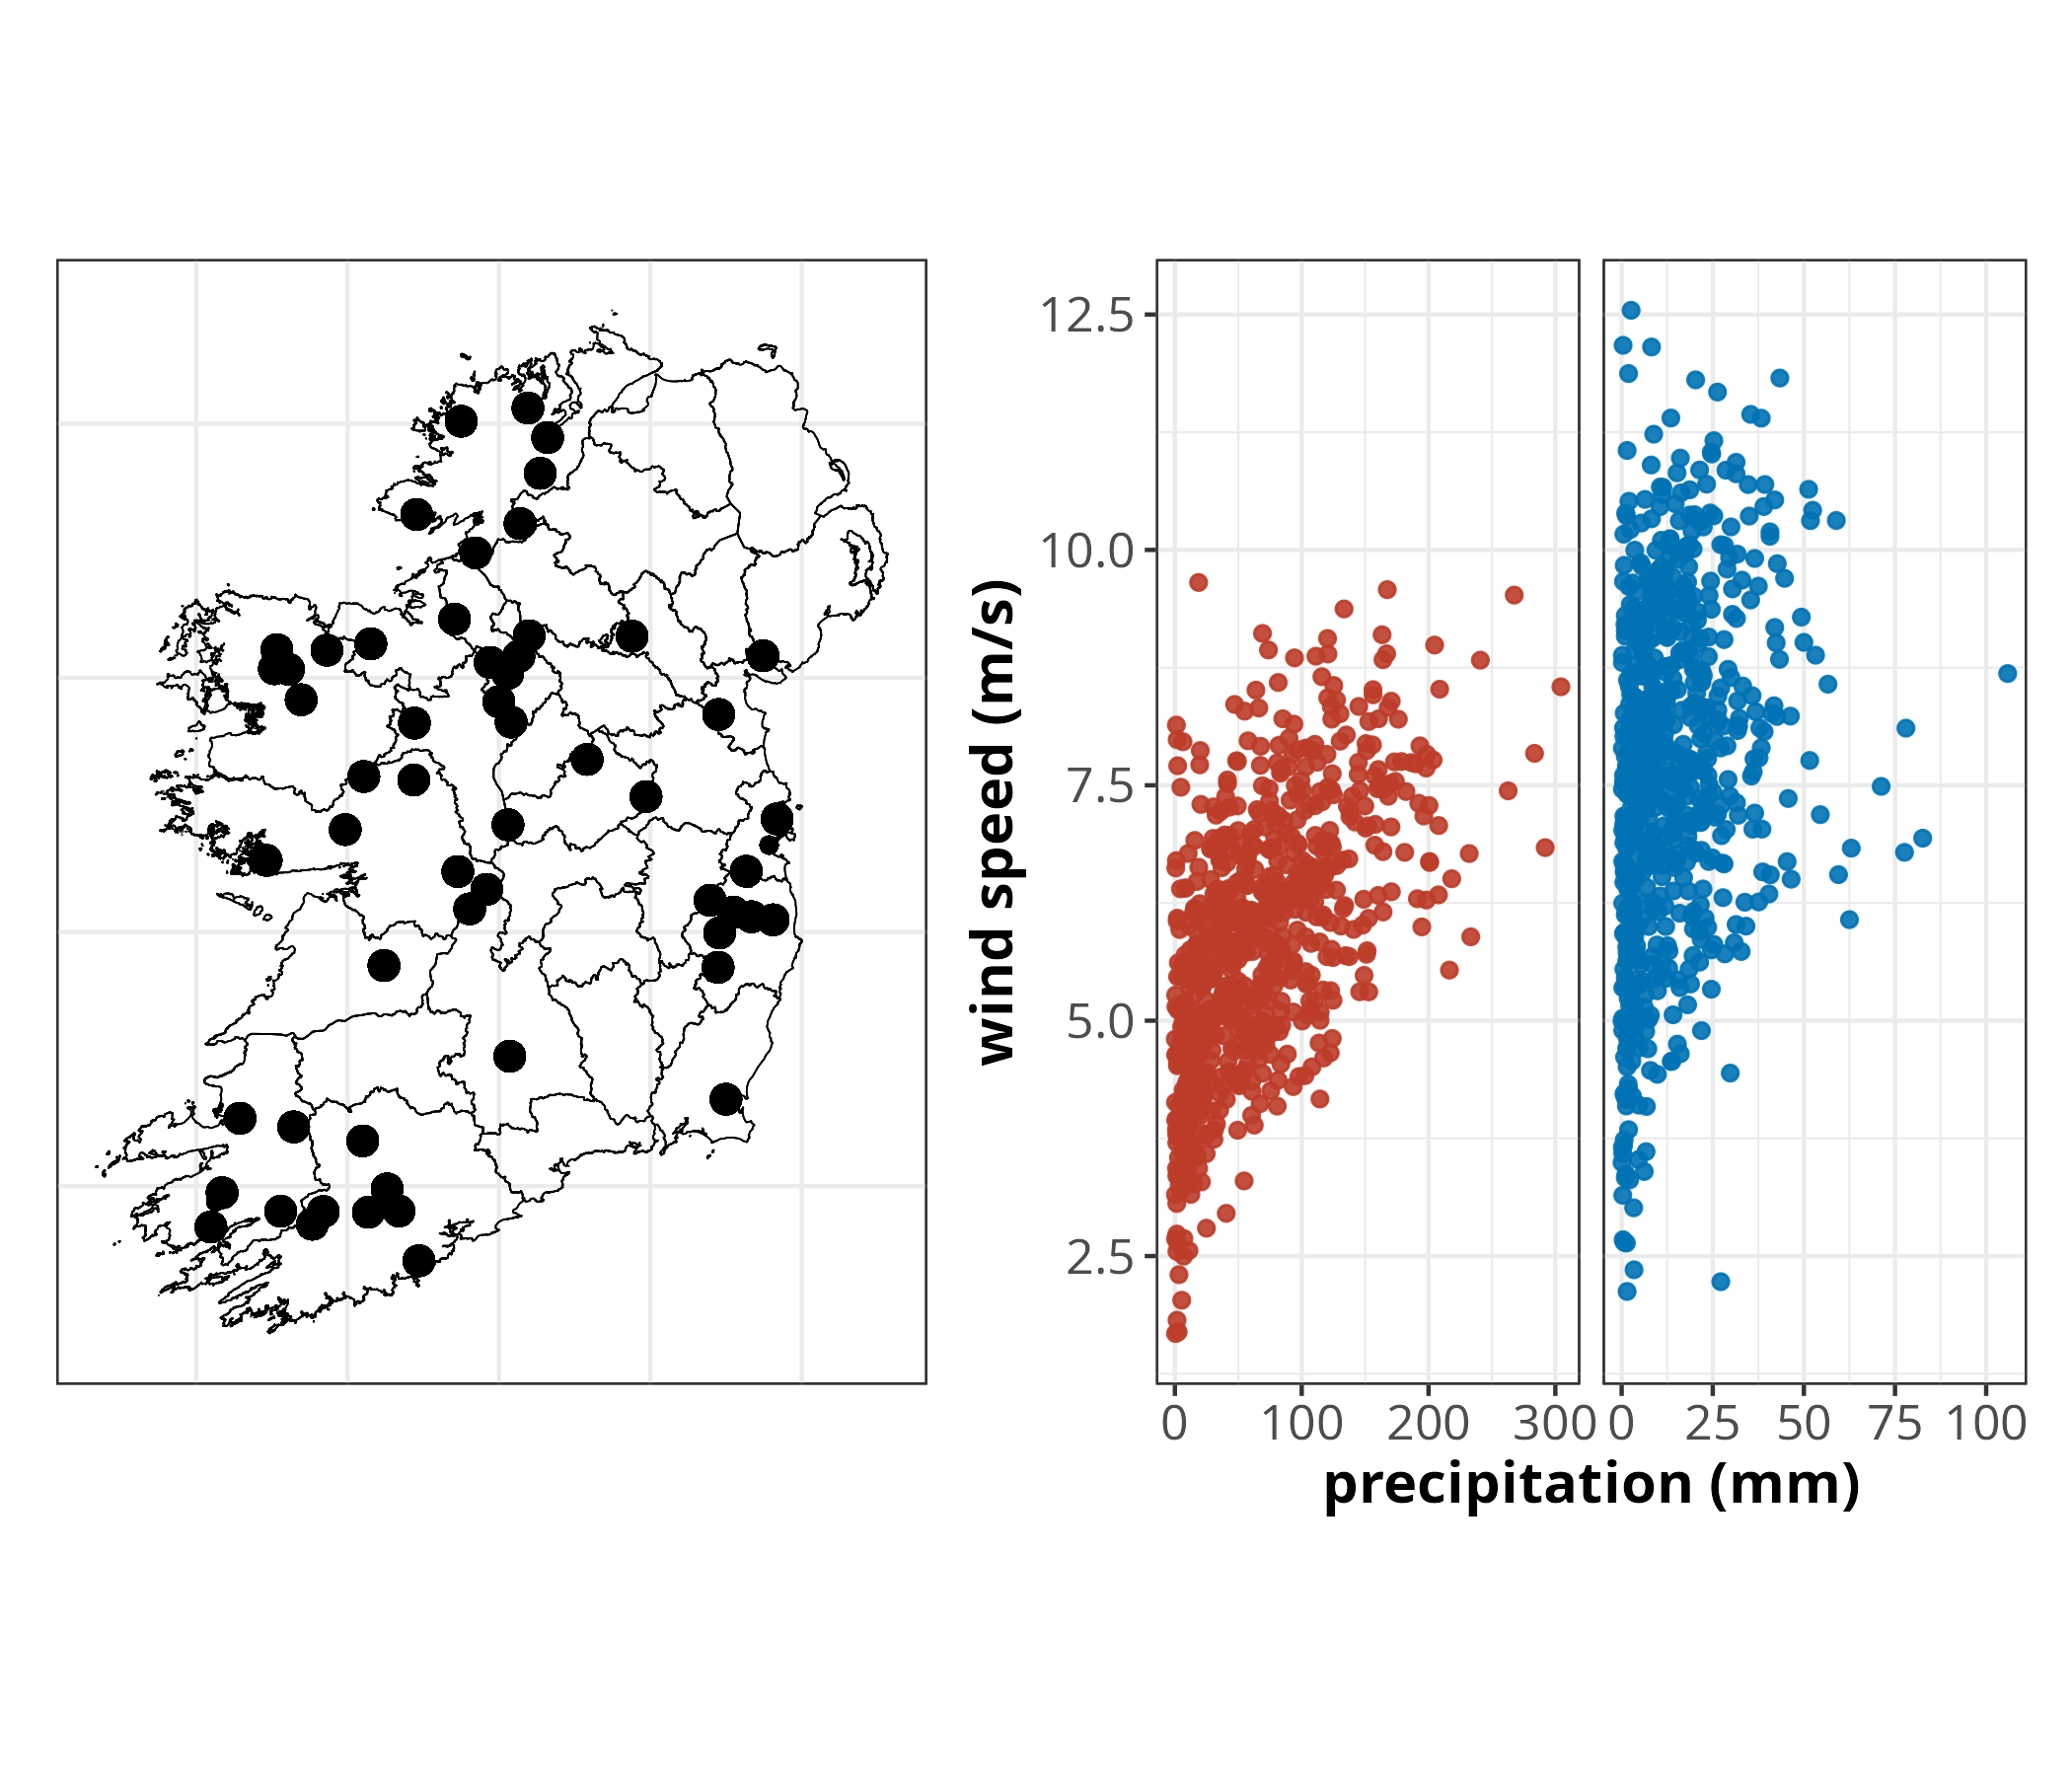
\includegraphics[width = 0.9\linewidth]{plots/02_mot_ex_plot.png}
    \caption{\emph{The figure on the left shows the location of 59 Met Éireann weather stations with precipitation data available from 1990 to 2020, inclusive. The points in red and blue show the weather sites at Cloone Lake in county Kerry and Ringsend and Dublin, which have the highest and lowest mean precipiation across this period, respectively. The figure on the right shows the weekly total precipitation in millimetres versus weekly wind speed maxima in metres per second for both of these sites.}}
    \label{fig:02_locs}
\end{figure}

% Introduce dataset
We consider extreme precipitation across ? weather sites in the Republic of Ireland from 1990 to 2020, inclusive.  

% Summaries of dataset

% Plot of locations on map, with wind speeds and precipitation for some
Include single exploratory plot to showcase data (left plot could have locations of weather sites, right could have precipitation plotted against wind speed for a given site).

Will now explain univariate extremes show how marginal models can be fit to this data.

\newpage
\section{Peaks-over-threshold method for univariate extremes}\label{sec:uni}

One classical approach to modelling univariate extremes, such as extremal precipitation or wind speed, is the peaks-over-threshold (POT) method, which uses the Generalised Pareto Distribution (GPD) to model exceedances over a high threshold.
In section \ref{subsec:uni_theory}, we first derive the GPD and describe in detail the modelling procedure for univariate extremes.
We expand on this methodology to more complex, non-stationary models in section \ref{subsubsec:non_stationary}, to formulate the method by which we will use in section \ref{subsec:uni_application} to model the univariate, marginal extremes of precipitation and wind speed in Ireland.

\subsection{Theory} \label{subsec:uni_theory}
% \todo{Add more here! Don't repeat what is above though}
\todo{How heavily should I relate this theory to our application?}
\todo{Reference Coles2001 once as a general reference for EVT, not multiple times}

Here, we will asymptotically motivate the use of the GPD, and describe the methods through which it can be used to model univariate extremes, ending in our non-stationary model for the marginal distribution for extremal precipitation and wind speed in Ireland.
Throughout this description, unless stated otherwise, we follow the general notation, illustration and definitions of \cite{Coles2001}.

\subsubsection{Block maxima asymptotic motivation} \label{subsubsec:asymptotic}

% \todo{Change to own words}
% \todo{Dupuis2023 has another good example of this, add reference}
% \todo{Must give GEV to justify GPD sigma, mean residual life linearity in u}
% \todo{Read Coles again to ensure everything we want to say is here}
% \todo{Why do we not have to estimate a and b here? Look at Coles 2001}
% \todo{Talk about block maxima more clearly}
% \todo{Talk about how Gz is referred to as an extreme value distribution}
\todo{Used Z to not confuse with X or Y in CE model, but Z is used as residuals?}
\todo{Is it clear that GEV is used to model maxima, not a single maximum?}

Extreme Value Theory is justified and motivated by the asymptotic basis upon which it relies.
% Following the illustration given in \cite{Coles2001}, suppose we have a sequence of independent and identically distributed (IID) random variables $Z_1, Z_2$ with common distribution function $F$. 
Suppose we have a sequence of independent and identically distributed (IID) random variables $Z_1, Z_2, \ldots$ with common distribution function $F$. 
% Let $M_n = \max(Z_1, \ldots, Z_n)$ be the ``block'' maximum of the first $n$ observations. 
Let $M_n = \max(Z_1, \ldots, Z_n)$ be the maximum of the ``block'' of size $n$.
Then $M_n$ is distributed as
\[
  \mathbb{P}(M_n \le z) = \prod_{i = 1}^{n}{\mathbb{P}(Z_i < z)} = \{F(z)\}^n.
\]
$F^n$ is difficult to recover from $F$ directly, as even slight inaccuracies in the estimate of $F$ can result in significant perturbations for $F^n$.
% \todo{Define as z up F as in Shooter2020 so we can use + below for GPD}
% Instead, we want to model $F^n$ directly by looking at its limiting behaviour as $n \to \infty$% , essentially as an extreme value analogue of the central limit theorem, which allows for the approximation of the distribution of sample means by the normal distribution. 
Instead, we model $F^n$ directly by looking at its limiting behaviour as $n \to \infty$.
Define the upper endpoint of F, as $z^F$. % , the smallest value such that $F(z^F) = 1$.
Then for any $z < z_F$, $M_n$ will degenerate to a point mass on $z_F$ as $n \to \infty$.
% This degeneration can be avoided by a linear normalisation of $M_n$:
% A non-degenerative sequence of maxima can be obtained by a linear renormalisation of $M_n$, such that
$M_n$ can be linearly renormalised to avoid this degeneration, such that
\[
  M_n = \frac{M_n - b_n}{a_n},
\]
for some sequences of normalising constants $a_n > 0, b_n$. 
\todo{Improve how this is stated to be in line with Dupuis2023?}
The Fisher-Tippet-Gnedenko theorem (\cite{Fisher1928}, \cite{Gnedenko1943}) states that, should such $a_n$ and $b_n$ exist, the limiting distribution of these non-degenerate maxima,
\begin{equation} \label{eq:uni_limiting_dist}
  \lim_{n \to \infty}\left\{\frac{M_n - b_n}{a_n}\right\} = G(z),
\end{equation}
is in the max-domain of attraction to, or must be, the Generalised Extreme Value (GEV) distribution, given by \todo{Need to be less formal/more clear?}
\todo{Need to write G z as H z | mu, sigma, xi?}
\begin{equation} \label{eq:gev}
  % G(z) = \exp\left\{-\left[1 + \xi\left(\frac{z - \mu}{\sigma}\right)\right]^{-1/\xi}\right\},
  G(z) = \begin{cases}
    \exp\left\{-\left[1 + \xi\left(\frac{z - \mu}{\sigma}\right)\right]_+^{-1/\xi}\right\} & \text{if } \xi \ne 0, \\
    \exp\left\{-\exp\left(-\frac{z - \mu}{\sigma}\right)\right\} & \text{if } \xi = 0,
  \end{cases}
\end{equation}
where $z_+ = \max(0, z)$, $z \in \mathbb{R}$, and $\mu \in \mathbb{R}, \sigma > 0$ and $\xi \in \mathbb{R}$ are location, scale, and shape parameters, respectively. 
These parameters absorb and implicitly incorporate the normalising constants, so they do not also have to be estimated. 
% For notes
% $a_n$ is a scaling factor and $b_n$ is a location adjustment that normalizes the maxima. 
% The GEV parameters absorb these scaling and shifting effects, which means that the estimation of $\mu$ and $\sigma$ serve the same purpose as estimating $a_n$ and $b_n$.
% The GEV distribution is so called because it is a family of distributions,
% incorporating the Gumbel, Frechet, and Weibull distributions as special cases
% for $\xi = 0, \xi > 0, \xi < 0$, respectively, which greatly simplifies
% estimation of the distribution. 
The limiting result in \ref{eq:uni_limiting_dist} holds under weak assumptions on the tail of $F$ for almost all continuous distributions \cite{Dupuis2023}. 
% This asymptotic argument is known as the ``block-maxima'' definition of extremes and forms the basis on which the field of EVT has developed.
This asymptotic argument is known as the ``block-maxima'' definition and forms the classical model for extremes. 
In practice, the block size $n$ is often taken to be a regularly spaced block of time, such as a year. % , and the maxima are taken over the samples of the random variable within each block.
For example, we may take the maximum daily precipitation over each year, and model these maxima with a GEV distribution.
% \todo{Relate to our application with example?}

\subsubsection{Peaks-over-threshold method} \label{subsubsec:pot}
% \todo{Describe how GPD is equivalent to GEV and has same shape but different scale}

% In constrast, GPD for excesses over threshold (Fisher, Tippet, Gnedenko)
From this block-maxima definition, another approach to EVT, which we will be focusing more on, can be derived.
The Pickands-Balkema-de-Haan theorem (\cite{Pickands1975}, \cite{Balkema1974}) states that should $M_n$ satisfy \ref{eq:uni_limiting_dist} and converge in distribution to the GEV distribution, then for any $Z = Z_i, 1 \le i \le n$ in our sequence, the distribution of exceedances $z > 0$ over a high threshold $u$ are approximated by the Generalised Pareto Distribution (GPD), defined as
\begin{equation} \label{eq:gpd}
  % \mathbb{P}(Z \le z + u \mid Z > u) = 1 - \left(1 + \xi \frac{z}{\sigma} \right)_{+}^{-1/\xi},
  \mathbb{P}(Z > z + u \mid Z > u) = \left(1 + \xi \frac{z}{\sigma} \right)_{+}^{-1/\xi},
\end{equation}
% \todo{Gives survival function here, as in CE model, not CDF, change?}
where $\xi$ is equal to the shape parameter $\xi_{GEV}$ of the equivalent GEV distribution, which is invariant to block size, and the scale parameter is reformulated such that $\sigma = \sigma_{GEV} + \xi(u + \mu_{GEV})$ and is also unchanged by block size as the changes in $\sigma_{GEV}$ and $\xi_{GEV}$ are self-compensating. %, thus absorbing $\mu$ and removing the need to estimate a location parameter for the GPD, although $u$ can be thought of as one. 
\todo{Are xi and sigma invariant to block size?}
The derivation of the GPD is covered in detail in section 4.2.2 of \cite{Coles2001}. 

This alternative definition is known as the ``peaks-over-threshold'' method for modelling extremes. 
In many applications, it is preferable to the block-maxima method, as logically there may be many observations within a single block which exceed so-called ``maxima'' in other blocks, and so the block-maxima method may be inefficient.
% For example, in countries with a temperate climate, such as Ireland, daily precipitation in Winter months may exceed a certain threshold on many days, and so the block-maxima method would be inefficient for modelling the extremes of precipitation.
For example, in temperate, oceanic climates such as Ireland, daily precipitation in Winter months may exceed a certain threshold, and the block maxima for Summer months, on numerous occasions, and so the block-maxima method would be inefficient for modelling the extremes of precipitation.

% \subsubsection{Shape parameter}

% \todo{Cut down on some detail, will remove subsubsection here later}
The upper tail behaviour of the GPD is largely determined by the shape parameter, with higher values for the shape parameter give higher probabilities of extreme events of greater magnitude. 
% Indeed, it determines the form of the distribution itself, with the Generalised Pareto distribution actually defining a ``family'' of distributions. 
% More detailed version
% When $\xi < 0$, the upper tail is said to follow the Weibull distribution, which is short-tailed and has a finite maximum bounded by the point $u - \sigma/\xi$. 
% As $\xi \to 0$, the GPD converges to the exponential distribution, and the distribution is said to be ``light-tailed'' with the right hand side of \ref{eq:gpd} being $ \approx 1/exp(-z)$ for large $z$, with no upper bound on the maximum.
% Finally, where $\xi > 0$, the upper tail is said to be follow a Pareto or heavy-tailed distribution, and the distribution function of the GPD is $\approx 1/z^{1/\xi}$ for large $z$, following a power-law upper tail decay with no upper bound. \cite{Rohrbeck2021} \cite{Carreau2017}.
For $\xi <0$, the upper tail is said to be Weibull distributed or short-tailed, and has a finite maximum at $u - \sigma/\xi$.
For $\xi \to 0$, the tail is exponentially distributed and is said to be light-tailed with no upper bound, while for $\xi > 0$, the tail is said to be Pareto distributed or heavy-tailed, and follows a slower, power-law decay, again with no upper bound \cite{Rohrbeck2021} \cite{Carreau2017}.

% \subsubsection{Return levels}

% \todo{Possibly move this motivation to intro}
% One of the principle and indeed unique uses of EVT is in the estimation of return levels, as outlined in \cite{Coles2001}. 
% Return levels are immensely useful as they give the expected value of the maximum observation of a random variable $Z$ over a number of observations or block of time, which may be an extrapolation over observed values. \todo{Word better!}
% For example, the 100-year return level for precipitation is the value which we expect to be exceeded on average once every 100 years. 
% \todo{Talk about how this is useful in applications, or should I do that in intro?}

% Return levels are estimated high quantiles beyond observed values, one of the principal uses of EVT. 

\todo{Shorten considerably}

In the context of extremes, we are often interested in return levels, which correspond to the expected value of the maximum observation of a random variable $Z$ over a number of observations or block of time.
This allows us to extrapolate modelled processes to values which have not been observed, and are useful in many applications.

% m-observation return level
The $m$-observation return level is the value of $Z$ which is expected to be exceeded on average once every $m$ observations.
% Long derivation
% We can derive this from the GPD by noting that the probability of $Z$ exceeding some value $z > u$ is given by
% \begin{align*}
%   \mathbb{P}(Z > z) &= \mathbb{P}(Z > z, Z > u) \\
%                     &= \mathbb{P}(Z > z \mid Z > u) \mathbb{P}(Z > u)
% \end{align*}
% % The first of these probabilities can be estimated by a GPD as in equation \ref{eq:gpd}, and the second is the exceedance probability for a given threshold $u$, which we define as $\zeta_u$, and can be estimated by, for example, a Binomial distribution.
% The first of these probabilities can be estimated by a GPD as in equation \ref{eq:gpd}, and the second, which we denote as $\zeta_u$, is the exceedance probability for a given threshold $u$, and can be estimated using a Binomial distribution.
% Therefore, the level $z_m$ exceeded on average every $m$ observations is the solution of 
% $\zeta_u \mathbb{P}(Z > z_m \mid Z > u) = 1/m$, which is given by
% \begin{equation} \label{eq:m_obs_return}
%   z_m = u + \frac{\sigma}{\xi}\left(\left(m \zeta_u \right)^{\xi} - 1\right),
% \end{equation}
% for $m$ large enough that $x_m > u$. 
Defining the exceedance probability for a given threshold $u$ as $\zeta_u = \mathbb{P}(Z > u)$, the $m$-observation return level is given by
\begin{equation} \label{eq:m_obs_return}
  z_m = u + \frac{\sigma}{\xi}\left(\left(m \zeta_u \right)^{\xi} - 1\right),
\end{equation}
where $\sigma$ and $\xi$ come from the corresponding GPD fit, and for $m$ large enough that $x_m > u$. 

% N-year
It is often more intuitive to express return levels in terms of years, and so we can also define the $N$-year return level.
For $n_y$ observations per year, we have that $m = N \times n_y$, and the $N$-year return level follows as
\begin{equation} \label{eq:n_year_return}
  z_N = u + \frac{\sigma}{\xi}\left(\left(N n_y \zeta_u \right)^{\xi} - 1\right). 
\end{equation}

\subsubsection{Threshold selection} \label{subsubsec:threshold}
\todo{Perhaps shorten, quite longwinded}
% Threshold selection methods (stability plots, automatic selection, quantile regression)
% Bias-variance tradeoff in threshold selection
% Can also work with extremal mixture models with so called "Bulk" distributions (as seen in marginal component of CE model)
% (see Rohrbeck2021)
% The threshold $u$ can also be thought of as a location parameter for this pdf, as for fixed $\sigma, \xi$, a change in $u$ will simply shift the distribution. \cite{Coles2001}
% The problem of threshold selection for the GPD is a difficult one, as the choice of threshold can have a large impact on the parameter estimates of the GPD, and presents a classic bias-variance trade-off. 
Threshold selection for the GPD presents a bias-variance tradeoff. 
\todo{Would like to somehow say this in a better way, making reference to asymptotic behaviour..}
% If $u$ is too small then the asymptotic justification on which the GPD relies becomes less valid, making it a less appropriate distribution for the data in question and introducing significant bias.
If $u$ is too small then the asymptotic justification for the GPD will not hold,  introducing significant bias.
% On the other hand, we require sufficient data to estimate the distribution. 
% Hence, too large a choice of $u$ will leave us with little data to numerically estimate the distribution with and result in high uncertainty in its parameters. 
In contrast, if $u$ is too large, we may have too little data to estimate the distribution with, resulting in high parameter uncertainty.
Classically, graphical methods have been employed for threshold selection.

% Mean residual life plot
% One classical method of threshold selection is the mean residual life plot. %, for which we follow the derivation in \cite{Coles2001}.  
\todo{Check that this is correct}
One such method is the mean residual life plot, the idea behind which we will now explore. \todo{Cite original paper this comes from?}
For a random variable $Z \sim GPD(\sigma, \xi)$, provided $\xi < 1$ the expected value of $Z$ is finite and $\mathbb{E}(Z) = \sigma/1 - \xi$.
Now suppose we have a series of random variables $X_1, X_2, \ldots, X_n$ for which excesses over a threshold $u_0$ follow a GPD. 
Then for any $X = X_i, 1 \le i \le n$, 
\[
  \mathbb{E}(X - u_0 \mid X > u_0) = \frac{\sigma_{u_0}}{1 - \xi},
\]
% where we denote the scale parameter corresponding to the threshold $u_0$ as $\sigma_{u_0}$, with $\xi$ being invariant for sufficiently high $u_0$. 
where $\sigma_{u_0}$ is the scale parameter corresponding to the threshold $u_0$, and $\xi$ is invariant as $u_0$ is sufficiently high.
If the GPD is valid for $u_0$, then for any threshold $u > u_0$, the GPD should also be valid.
Then from section \ref{subsubsec:pot}, $\sigma_u = \sigma_{u_0} + \xi(u_0 + \mu)$, with $\mu = 0$ for the GPD, and we have that \todo{Is this clear enough? Was first in reference to GEV}
\begin{align} \label{eq:lin_u}
  \begin{split}
  \mathbb{E}(X - u \mid X > u) &= \frac{\sigma_u}{1 - \xi} \\
                                   &= \frac{\sigma_{u_0} + \xi u_0}{1-\xi}.
  \end{split}
\end{align}
Hence, for $u > u_0$, this expectation is a linear function of $u$. 
Furthermore, we can say that this expectation is the mean of the excesses over $u$, which is estimated by the sample mean. 
% Hence, we can plot the mean excesses over a series of thresholds, and if the GPD is valid for a given threshold, we should see a linear relationship between the mean excesses and the threshold.
Hence, the mean residual life plot takes as points a series of thresholds $u$ and the correspoding sample mean of the excesses over each threshold, plotting
\[
  \left\{\left( u, \frac{1}{n_u} \sum_{i=1}^{n_u}{\left(z_i - u\right)}: u < z_{F} \right) \right\},
\]
where $n_u$ is the number of excesses over the corresponding threshold $u$.
For valid choices of $u$, we should see a linear relationship between the mean excesses and the threshold, and in practice we try to choose the smallest $u$ which gives this linear relationship, preserving as much data as possible for the estimation of the GPD.

Following a similar logic, for sufficiently large choices of $u$, the values of $\xi$ should be constant and the values of $\sigma$ should be linear in $u$, as in equation \ref{eq:lin_u}.
This is the basis for the second classical method of threshold selection, the so-called ``threshold choice'' plot.

% Newer developments
% Other classical methods that focus instead on diagnosing the fit of a GPD for a given threshold to data are discussed in section \ref{subsubsec:uni_diagnostics}.
These earlier, graphical methods, however, are rather subjective.
There have been many more recent advances in the field of threshold selection, aiming to provide more subjective methods. 
A review of many alternative threshold selection methods can be found in section 2.6 of \cite{Belzile2022}, including methods focused on formal testing of a GPD for a given $u$ against an alternative model, and evaluating predictions of unseen data, such as leave-one-out cross-validation (CV). \todo{Need for section?}

% However, many of these techniques are entirely manual, and so are quite laborious in the context of fitting multiple marginal models to, for example, different variables or spatial locations.
However, many of these techniques are still quite manual, and in the face of this, the area of ``automatic'' threshold selection is a growing area of research. 
One such method is that described in \cite{Murphy2024}, where the GPD is repeatedly fit over various choices of $u$ based on the quantiles of the data, and the optimal choice of threshold is taken to be that which minimises the so-called expected quantile discrepancy (EQD).
% This method has been shown to be robust in the face of the bias-variance trade-off problem, when compared to other means of automatic threshold selection, and is less subjective than the plotting methods described above. 
This method is less subjective than the plotting methods described above.
In \ref{subsubsec:non_stationary}, we will discuss another method for automatic threshold selection through quantile regression, which is useful when we want to estimate thresholds across different times and/or spatial locations.

\subsubsection{Non-stationary modelling} \label{subsubsec:non_stationary}
% Including covariates, using evgam, Gaussian processes, INLA in spatial context
% to reflect non-linearity of spatial effects
% \todo{Cooley2007 uses Gaussian process}
% \todo{See Rohrbeck2021 for nice write up about this}
\todo{Section probably too long, cut down!}

% Introduction  
% Recall that the asymptotic motivations for EVT from \ref{subsubsec:asymptotic} assumes that the distribution of the random variables $Z_1, Z_2, \ldots$ are I.I.D and stationary.
The asymptotic justification for EVT in section \ref{subsubsec:asymptotic} assumes that the sequence $Z_1, Z_2, \ldots, Z_n$ are IID stationary.
% In practice, this is often not a realistic assumption, since their values may be influenced by some covariates, such as spatial location or time.
This assumption can often be unrealistic in practice, 
There are many methods for handling this non-stationarity. 
One method is to split the data into separate time series over which we deem the data to be stationary, and fit separate GPDs to each of these series.
Another method which often makes better use of the available data is to model the parameters of the GPD as functions of covariates. 
% For simplicity, we use spatial location $s \in S$ as our covariate, and $Z(s)$ as the process sampled at location $s$, since this is what is used in our motivating example. 
For simplicity of exposition, and to link to our motivating example, our covariate will be spatial location $s \in S$, denoted a process sampled at location $s$ as $Z(s)$.

% Quantile regression for threshold
As mentioned in \ref{subsubsec:threshold}, the exceedance threshold $u$ can be modelled as a function of covariates using quantile regression, as developed in \cite{Yu2001} and outlined in the context of extremes in \cite{Youngman2019}.
% Quantile regression estimates $u$ as a function of some covariates, $\bm{x}$, which could include spatial location and/or time, as a prespecified quantile of the data $\tau$. \todo{Need to define x more clearly}
Extremal quantile regression estimates the threshold as a prespecified quantile $\tau$ of the data. 
The random variable $Z(s)$ can be modelled with an asymmetric Laplace distribution (ALD).
Following \cite{Youngman2019} the parameters of said distribution can be modelled as smoothed basis functions, and we have that
% \begin{equation} \label{eq:asymmetric_laplace}
%   Z(s) \mid u(s), \psi(s) \sim ALD(u(s), \psi(s)),
% \end{equation}
\begin{center}
  \begin{align} \label{eq:asymmetric_laplace}
    \begin{split}
      Z(s) \mid u(s), \psi(s) &\sim ALD(u(s), \psi(s)), \\
      % \log{\psi(s)} &= u_0 + \sum_{k = 1}^{K_{\psi}}{\sum_{d = 1}^{D_k_{\psi}}\beta_{kd}(s)},
      % u(s) &= u_0 + \sum_{k = 1}^{K_u}{\sum_{d = 1}^{D_k{_u}}\beta_{kd}(s)}, \\
      u(s) &= f_u(s), \\
      \log(\psi(s)) &= f_{\psi}(s), \\
      f_*(s) &= \beta_0 + \sum_{k = 1}^{K_*}{\sum_{d = 1}^{D_k{_*}}\beta_{kd}b_{kd}(s)}, \\
    \end{split}
  \end{align}
\end{center}
where $u(s)$ is the quantile $0 < \tau < 1$ of the data at location $s$, $\psi(s) > 0$, and $f_*(s)$ is the smooth function across space for either $u$ or $\psi$ with associated intercept $\beta_0$ and basis functions $b_kd$ with corresponding parameters $\beta_{kd}$.
Using a log link function ensures that $\psi(s) > 0$.
The use of basis functions and GAMs is described further surrounding equation \ref{eq:gpd_gam} below. 
Likelihood methods allow us to estimate $u(s)$ from this model, giving us a threshold above which to define extreme values of $Z(s)$.
This method allows us to easily estimate thresholds for a high-dimensional dataset characterised by covariates such as spatial location.

% Non-stationary GPD
% Furthermore, we can also model the parameters of the GPD as functions of covariates such as $s$.
Furthermore, we can also model the GPD parameters using covariates.
Un
% Under this model, equation \ref{eq:gpd} becomes
%   \mathbb{P}(Z((s)) > z + u(\bm(x)) \mid Z > u, s) = \left(1 + \xi(s) \frac{z}{\sigma(s)} \right)_{+}^{-1/\xi(s)}.
% \end{equation}
For example, we could assume that the scale and shape parameters of the GPD are linear functions of $s$.
Under this model, we could model threshold exceedances at location $s$ as 
\begin{center}
  \begin{align} \label{eq:non_stationary_gpd}
    \begin{split}
      Z(s) - u(s) \mid Z(s) > u(s) &\sim GPD(\sigma(s), \xi(s)), \\
                   \log(\sigma(s)) &= \sigma_0 + \sigma_1 s, \\
                            \xi(s) &= \xi_0 + \xi_1 z(s),
    \end{split}
  \end{align}
\end{center}
where $\sigma_0, \sigma_1, \xi_0, \xi_1$ are intercept and slope parameters for the scale and shape, respectively, and $u(s)$ is modelled as in equation \ref{eq:asymmetric_laplace}.
% Using a log link function ensures that $\sigma(s) > 0$.
% This model, which can be made as complicated as necessary, allows for much greater flexibility in our models, and reduces the bias associated with assuming a constant shape and scale parameter across all locations.
This model allows for much greater flexibility, and reduces the bias associated with assuming a constant shape and scale parameter across all locations.
% However, it is important to note that as always, there is a variance trade-off here as well, as in this example, estimating a GPD at each location will require more data than estimating a single GPD for all locations.
However, there is a variance tradeoff associated with estimating a GPD at each location, where less data is available than for a single GPD for all locations.
In particular, the shape parameter is often difficult to estimate, and so in practise in spatial and spatio-temporal applications it is often assumed to be constant across locations, or be the same for a group or cluster of different locations \cite{Cooley2007}, \cite{Rohrbeck2021}, and also often fixed over time \cite{Risser2019} \cite{Zhang2024}. 
% This tradeoff has motivated research into clustering or grouping locations into groups which share similar characteristics and GPD parameters, as discussed in section \ref{sec:clustering}.
% \todo{Motivate clustering here?}

\todo{Cut down sections here}
% Gaussian processes
% There are several more advanced, non-linear methods for modelling non-stationary GPDs.
% One of these is the use of a Gaussian process (GP), as in \cite{Cooley2007}, where the scale parameter was modelled as an isotropic GPs with a mean function depending on various spatial and climatic covariates, and a covariance function given by an exponential variogram, allowing for the spatial dependence of the scale parameter to be modelled.
% The non-parametric nature of GPs mean they can capture complex, non-linear spatial patterns in the scale parameter.

% % INLA
% Another method for estimating a non-stationary GPD is using the Integrated Nested Laplace Approximation (INLA), a method for approximate Bayesian Inference popular in spatial statistics \cite{Rue2009}.
% The GPD was shown to fit the class of latent Gaussian models required of INLA, and implemented for the \texttt{R-INLA} R package in \cite{Opitz2018}.
% R-INLA is a powerful tool for fitting complex, non-linear models to spatial data, with many spatial and spatio-temporal random and mixed-effects models available, and performs particularly well for high dimensional geostatistical data. 
% In particular, \cite{Opitz2018} implemented a penalised complexity prior for the shape parameter, which penalises deviation from the exponential model where $\xi = 0$, encouraging lighter tails \cite{Simpson2015}.

% GPs and INLA
There are several more advanced, non-linear methods for modelling spatially non-stationary GPDs.
\cite{Cooley2007} uses a Gaussian process to nonparametrically model the non-linear, complex spatial patterns in the scale parameter.
% \cite{Opitz2018} implements the GPD using the Integrated Nested Laplace Approximation (INLA) of \cite{Rue2009} for approximate Bayesian inference using a variety of spatial mixed- and random-effects models for the GPD which 
\cite{Opitz2018} implements the GPD using the Integrated Nested Laplace Approximation (INLA) of \cite{Rue2009} for approximate Bayesian inference.
A variety of spatial mixed- and random-effects models using, for example, autoregressive priors, are available which can exploit the spatial structure of the scale parameter.
Also, \cite{Opitz2018} uses a penalised complexity prior for the shape parameter, where significant deviation from the exponential model is penalised, encouraging lighter tails \cite{Simpson2015}.

% evgam
\todo{change wording from ITT2 report}
% Finally, the method we will use is fitting generalised additive models (GAMs) to the parameters of the GPD, using the \texttt{evgam} R package used and developed in \cite{Youngman2019} and \cite{Youngman2023}.
A GAM is a more flexible extension of the Generalised Linear Model (GLM) which allows the response to depend linearly on smooth functions, called basis functions, of some predictors \cite{Wood2006}.
The method we will be using for our motivating example is modelling the scale and shape parameters of the GPD as smooth functions of spatial location using generalised additive models (GAMs), using the \texttt{evgam} R package \cite{Youngman2022}.
The extreme value GAM model we use for both extreme precipitation and wind speed in section \ref{subsec:uni_application} is
\begin{center}
  \begin{align} \label{eq:gpd_gam}
    \begin{split}
      Z(s) - u \mid W(s) > u &\sim GPD(\sigma(s), \xi) \\
      % Z(s) \mid u(s), \psi(s) &\sim ALD(u(s), \psi(s))  \\
      \log{\sigma(s)} &= f_{\sigma}(s), \\
              \xi(s) &= f_{\xi}(s), \\
              f_*(s) &= \beta_0 + \sum_{k=1}^{K_*}b_k(s)\beta_k,
    \end{split}
  \end{align}
\end{center}
where $u(s)$ is as in equation \ref{eq:asymmetric_laplace} and $f_*$ is a smooth function of the spatial location $s$ for either $\sigma$ or $\xi$, modelled as a linear function of an intercept term $\beta_0$ and $K_*$ basis functions $b_k$ with corresponding coefficients $\beta_k$. 
A popular choice of basis function, which we have elected to use here, is the cubic spline, a curve constructed from interconnected segments of cubic polynomials, ensuring the curve's continuity up to its second derivative \cite{Wood2006}. 
This model, while simple to formulate and implement, allows for complex, non-linear patterns in the GPD parameters to be smoothed over space.

\subsubsection{Model diagnostics} \label{subsubsec:uni_diagnostics}
\todo{Cut down on detail here as well?}
% There are several methods described in \cite{Coles2001}, amongst other sources, for diagnosing the fit of a GPD to data, which are useful for threshold selection and model validation.
There are numerous methods for diagnosing the fit of a GPD to data, which are useful for  model validation and also threshold selection.
Suppose we have $k$ ordered threshold exceedances $z_{(1)} < z_{(2)} < \ldots < z_{(k)}$.
The probability plot consists of the points
\begin{equation} \label{eq:prob_plot}
  \left\{ \left(i/(k + 1), \hat{H}\left(z_{(i)}\right)\right); i = 1, 2, \ldots, k \right\}, 
\end{equation}
where $\hat{H}(z)$ is the cumulative distribution function (CDF) of the GPD, equivalent to 1 - equation \ref{eq:gpd}, for the corresponding parameter estimates $\hat{\sigma}$ and $\hat{\xi}$. \todo{Need to spell out with Hz is?}
For a good fit to the data, these points should be approximately linear.

The quantile plot shows the points
\begin{equation} \label{eq:quantile_plot}
  \left\{ \left( \hat{H}^{-1}(i/(k+1)) , y_{(i)}\right); i = 1, 2, \ldots, k \right\},
\end{equation}
where $\hat{H}^{-1}$ is the estimated quantile function of the GPD.
Again, the quantile plot should be approximately linear for a good fit.

The $n$-year return levels as described in equations \ref{eq:n_year_return} are often plotted on the log scale against year with empirical estimates included for comparison, to understand the long term extrapolation of the model and how well these fit the observed data. For a non-stationary fit such as that described in \ref{subsubsec:non_stationary}, the return levels will also be non-stationary and so can be plotted against covariates to understand how they relate.
% \todo{Link to return level equation once written}

Finally, a density curve for the fitted GPD can also be overlaid on the histogram of exceedance values to assess the fit of the GPD to the data.

\todo{Talk about need to estimate parameter uncertainty? Not done below!}
Another important aspect of model diagnostics is the estimation of parameter uncertainty, which is often overlooked in the context of GPDs, where uncertainty often high.
In the Bayesian setting, we can sample from the estimated posterior distributions of the parameters to estimate uncertainty, and in the Frequentist setting this can be done by bootstrapping the data and refitting the GPD to each bootstrap sample, giving a distribution of parameter estimates.

\subsection{Application to motivating example} \label{subsec:uni_application}
% \begin{itemize}
%   \item uses \texttt{evgam} to estimate $\sigma, \xi$ at each location smoothing both over space (can take from ITT2 report) for GPDs fitted to precipitation and wind speed, respectively.
%   \item Also uses method from \cite{Youngman2019} whereby location-specific thresholds are defined as fixed quantiles and estimated by quantile regression.
%   \item Show maps of $\sigma$ and $\xi$ for both rain and wind speed, $\ldots$ (what else?)
%   \item Possibly show uncertainty in $\xi$ estimates from vanilla \texttt{texmex}, or can I get uncertainty in \textbf{evgam} estimates for $\xi$ (see \cite{Youngman2023})?
%   \item QQ plots for GPD fits, showing how well the model fits the data (also
%   add histogram and return levels? Will need to fix from texmex plots) \todo{Add uncertainty to plots! From ITT2}
% \end{itemize}

\todo{Follow Youngman2019 for narrative and comments to be made}

% Threshold plot
\todo{Cutout whitespace in plot!}
\begin{figure}[H]
    \centering
    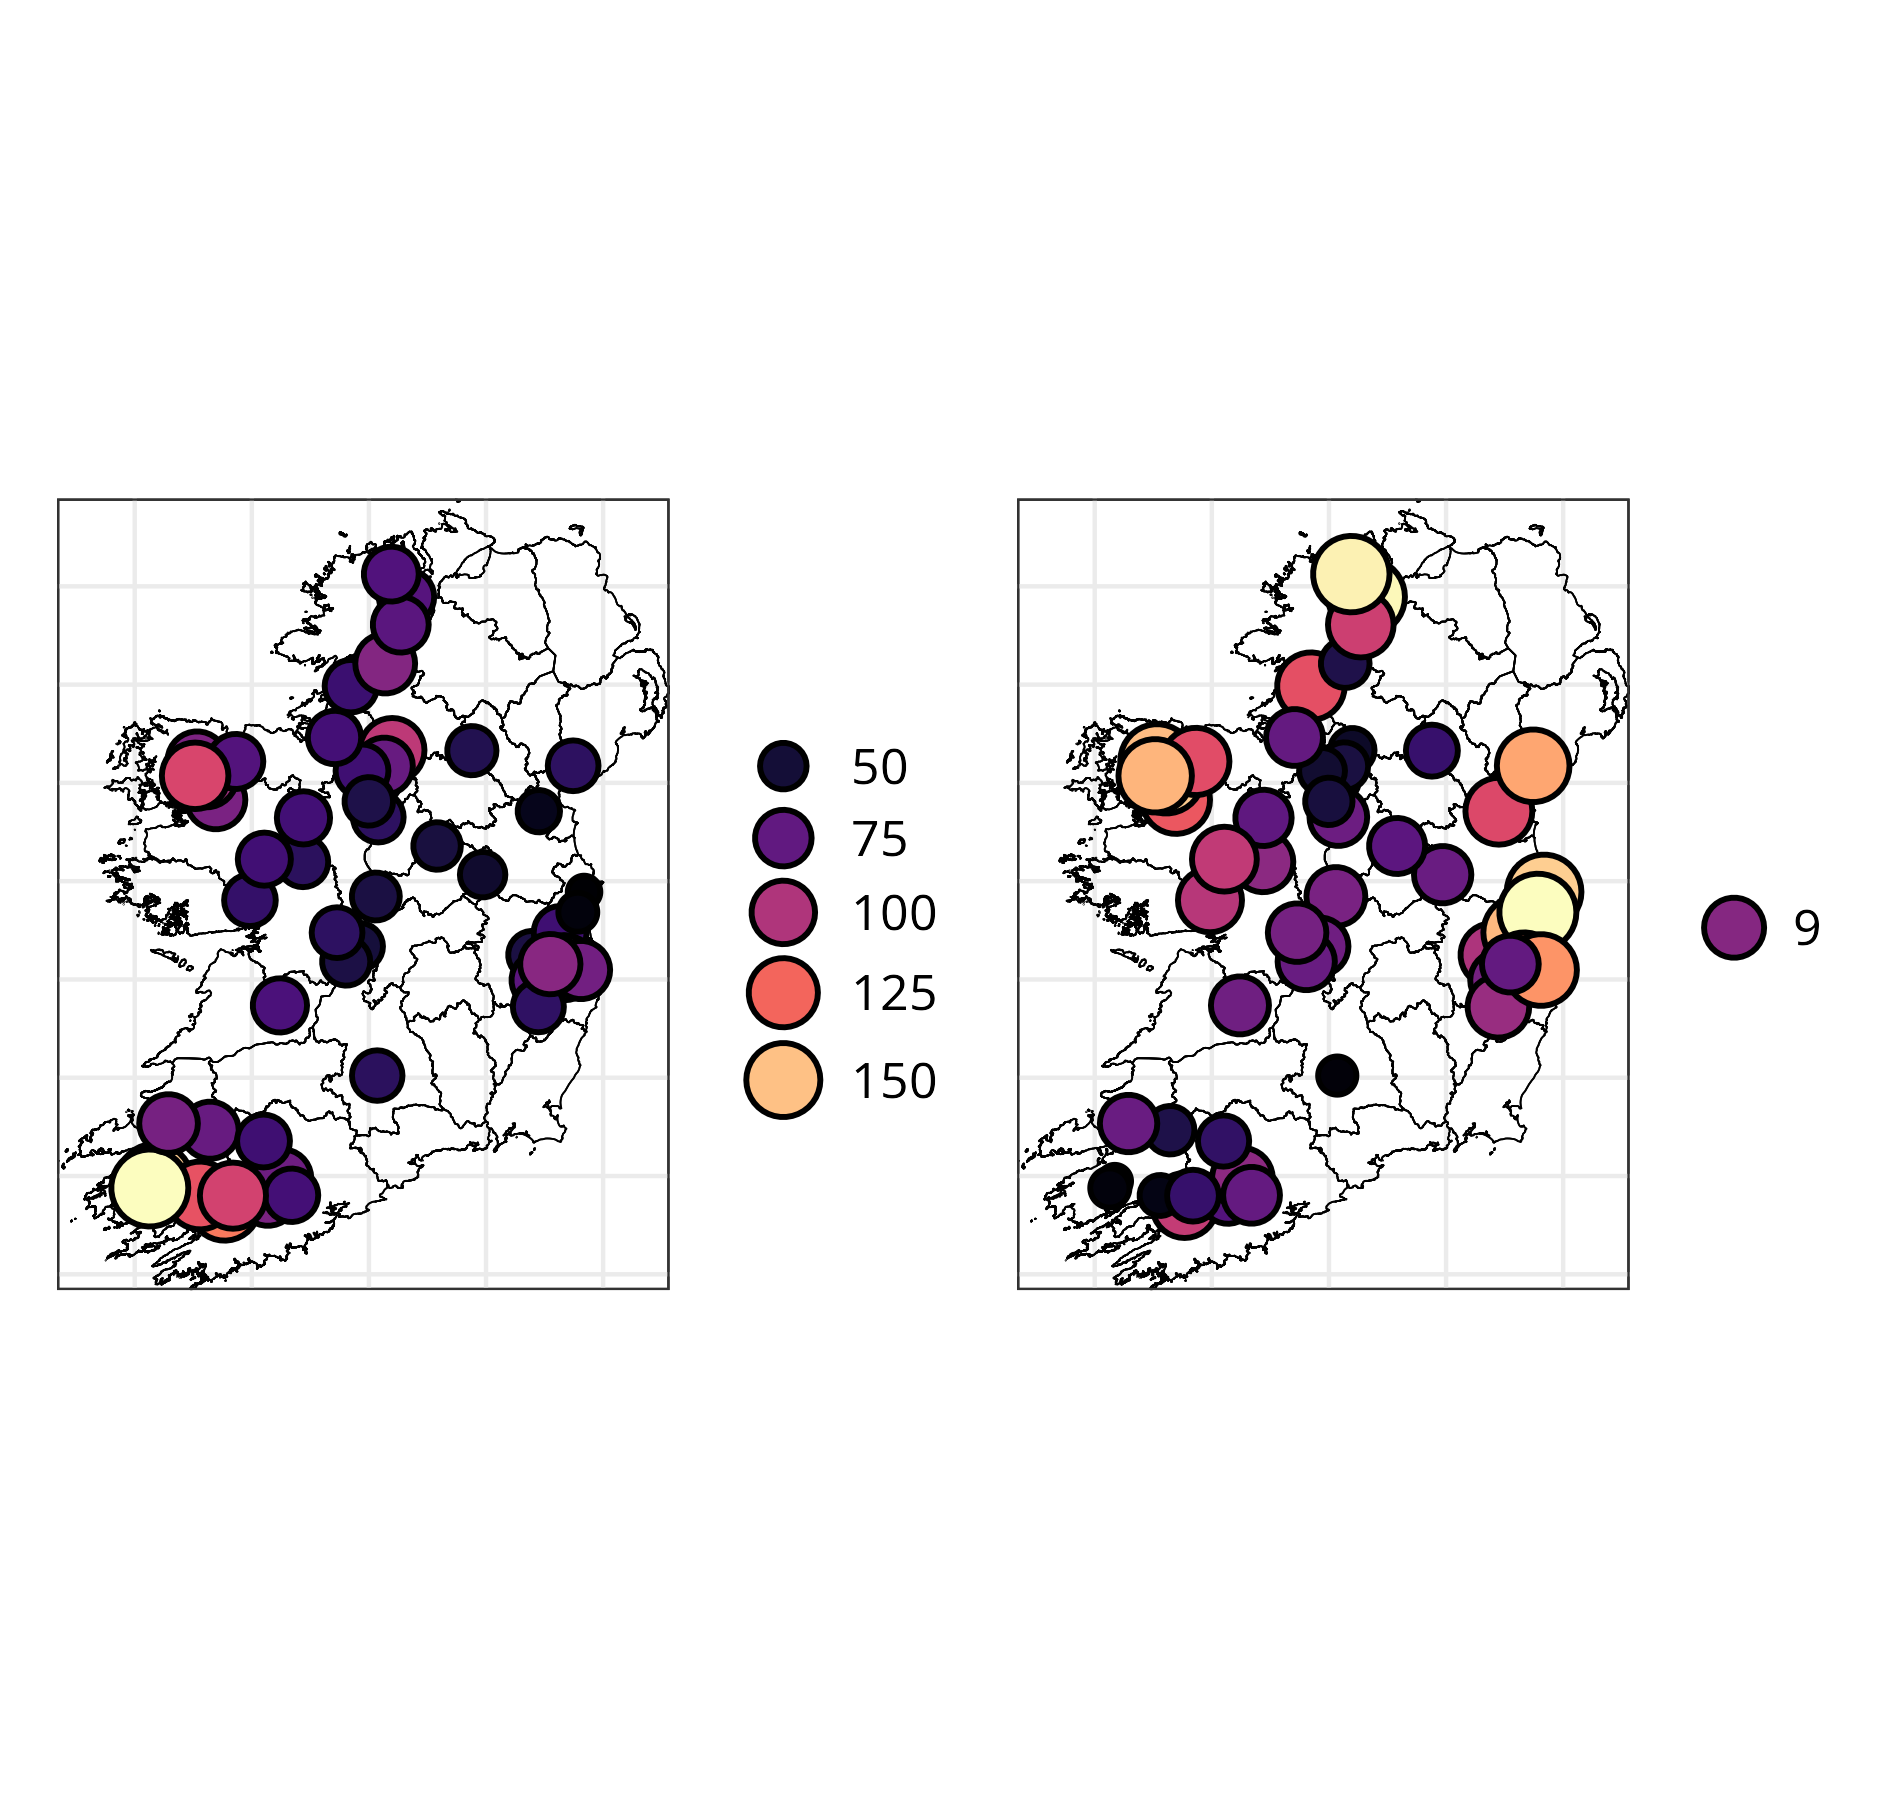
\includegraphics[width = 0.9\linewidth]{plots/031_thresh_plots.png}
    \caption{\emph{Figures, from left to right, show the Generalised Pareto Distribution thresholds for rain and wind speed, respectively, for each Met Éireann weather station.}}
    \label{fig:03_uni_thresh}
\end{figure}

% Method with evgam and quantile regression for threshold selection, to allow
% threshold to vary for different areas. 

% Parameters for rain
\begin{figure}[H]
    \centering
    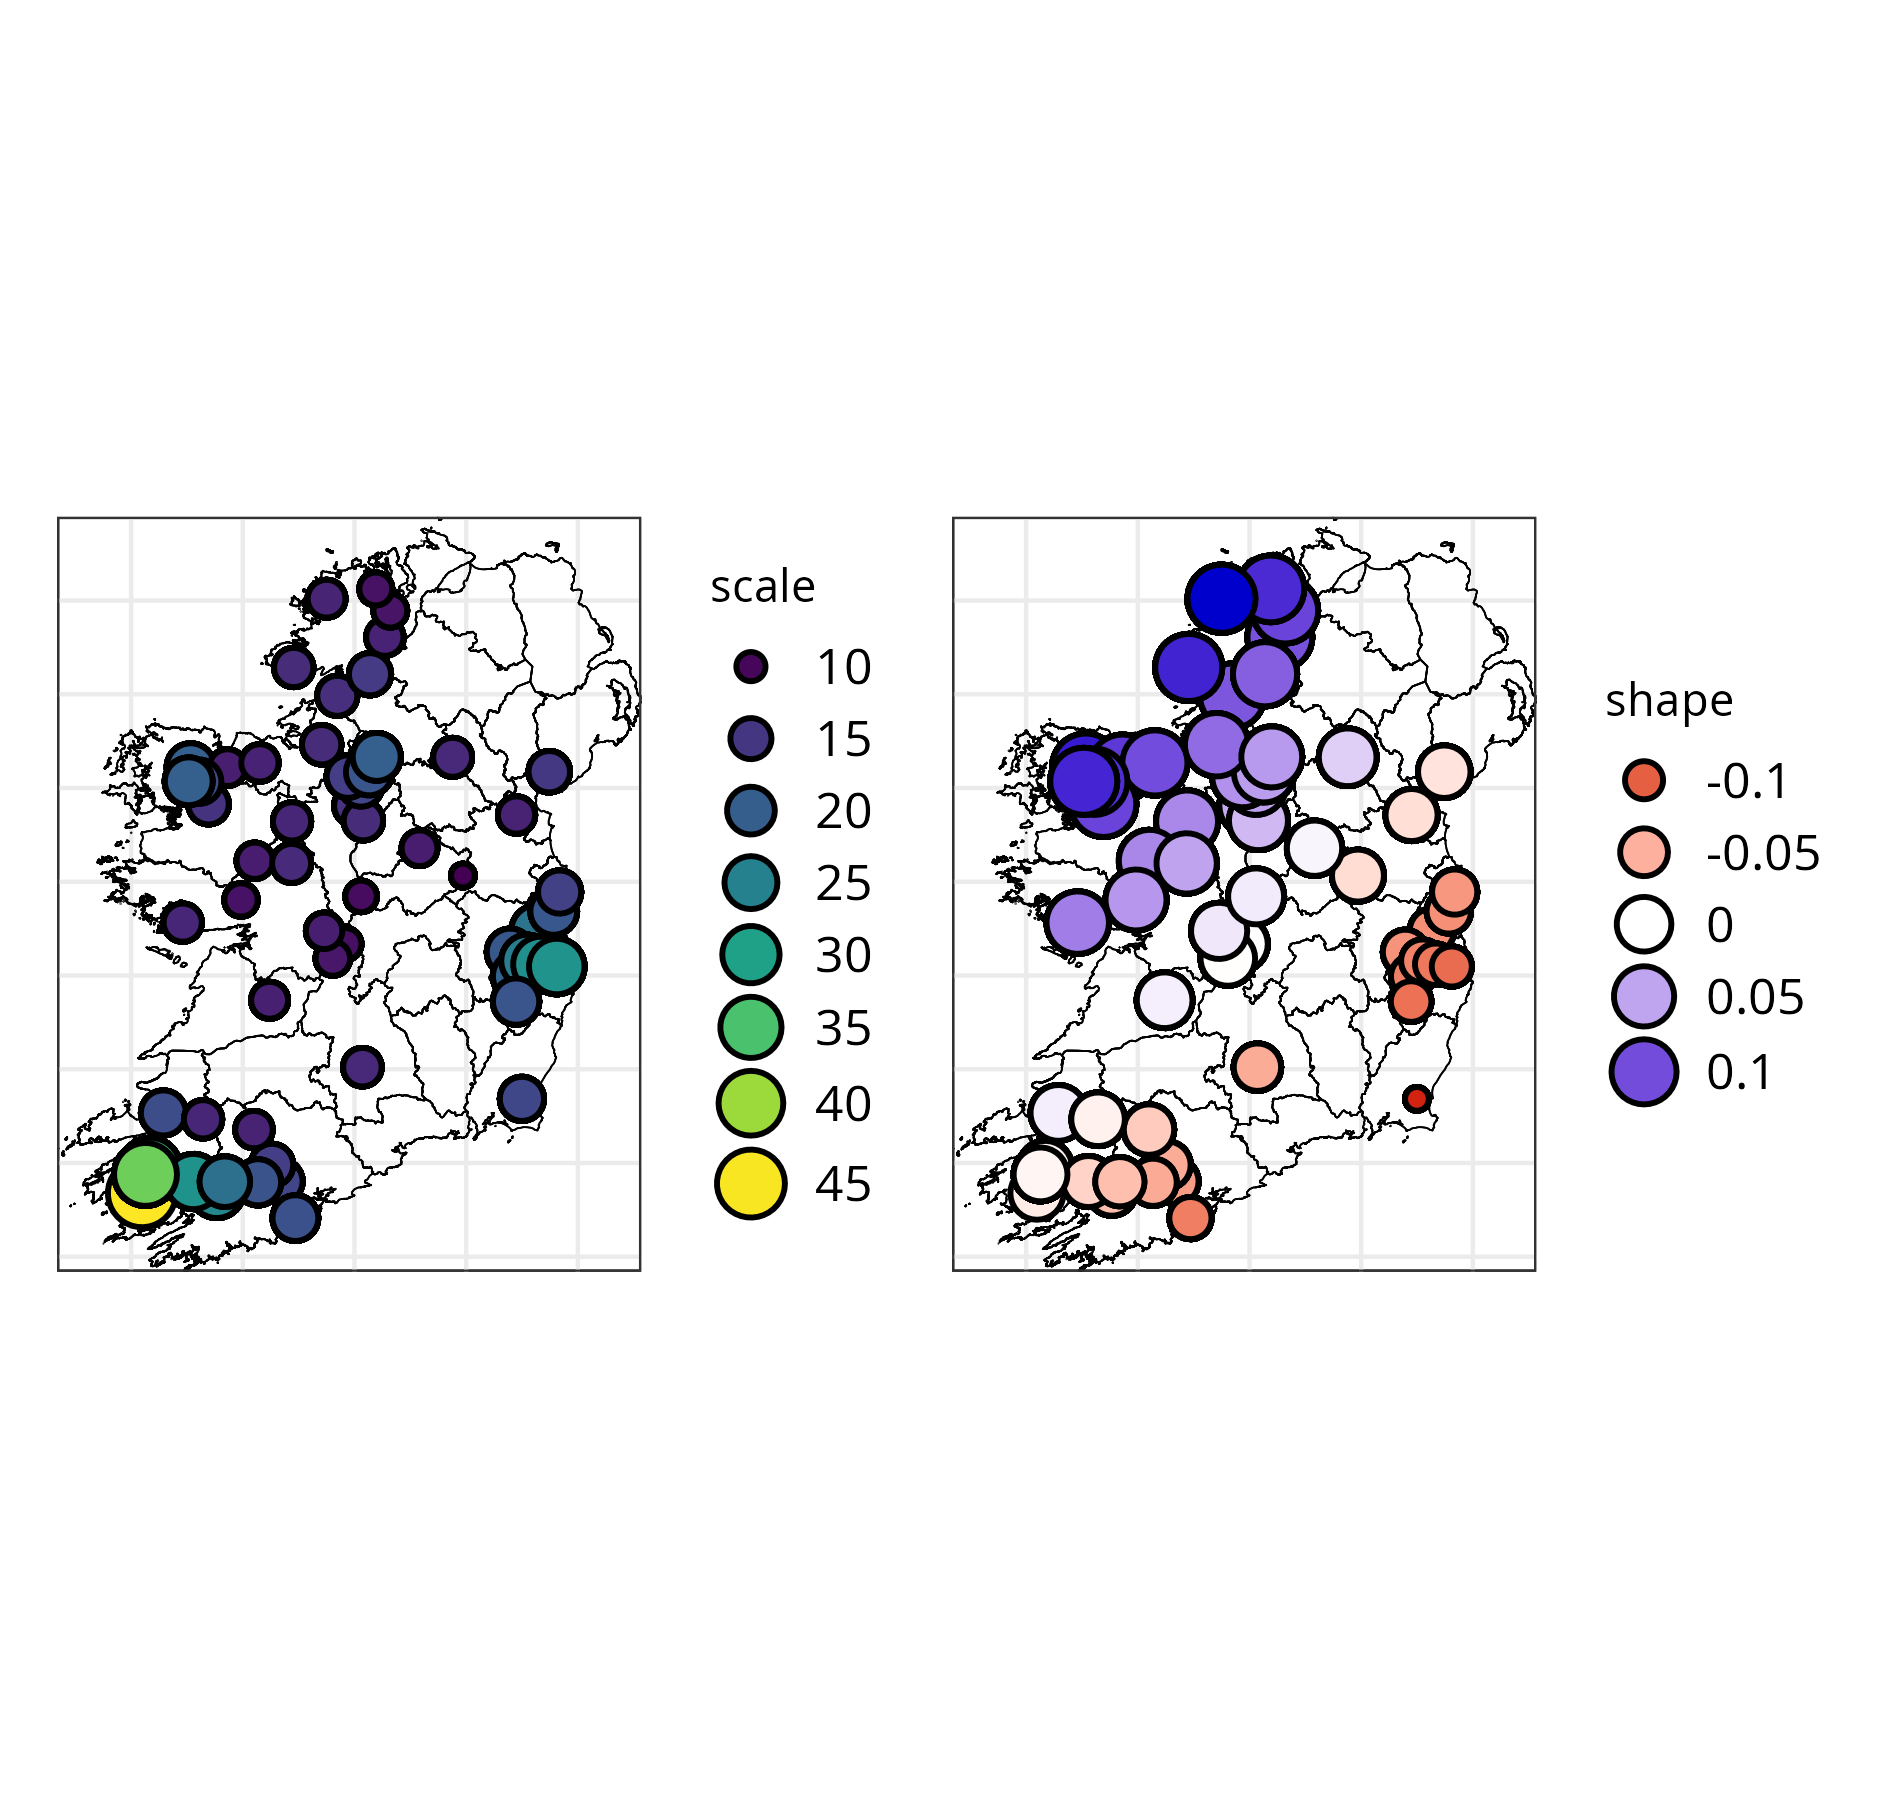
\includegraphics[width = 0.9\linewidth]{plots/032_gpd_rain.png}
    \caption{\emph{Figures, from left to right, showing the scale ($\sigma_rain)$ and shpa e($\xi_rain$) parameters of the Generalised Pareto distribution for weekly sums of precipitation at each Met Éireann weather station.}}
    \label{fig:03_gpd_rain}
\end{figure}

% Parameters for wind speed
\todo{Fix latex, not showing correctly!}
\begin{figure}[H]
    \centering
    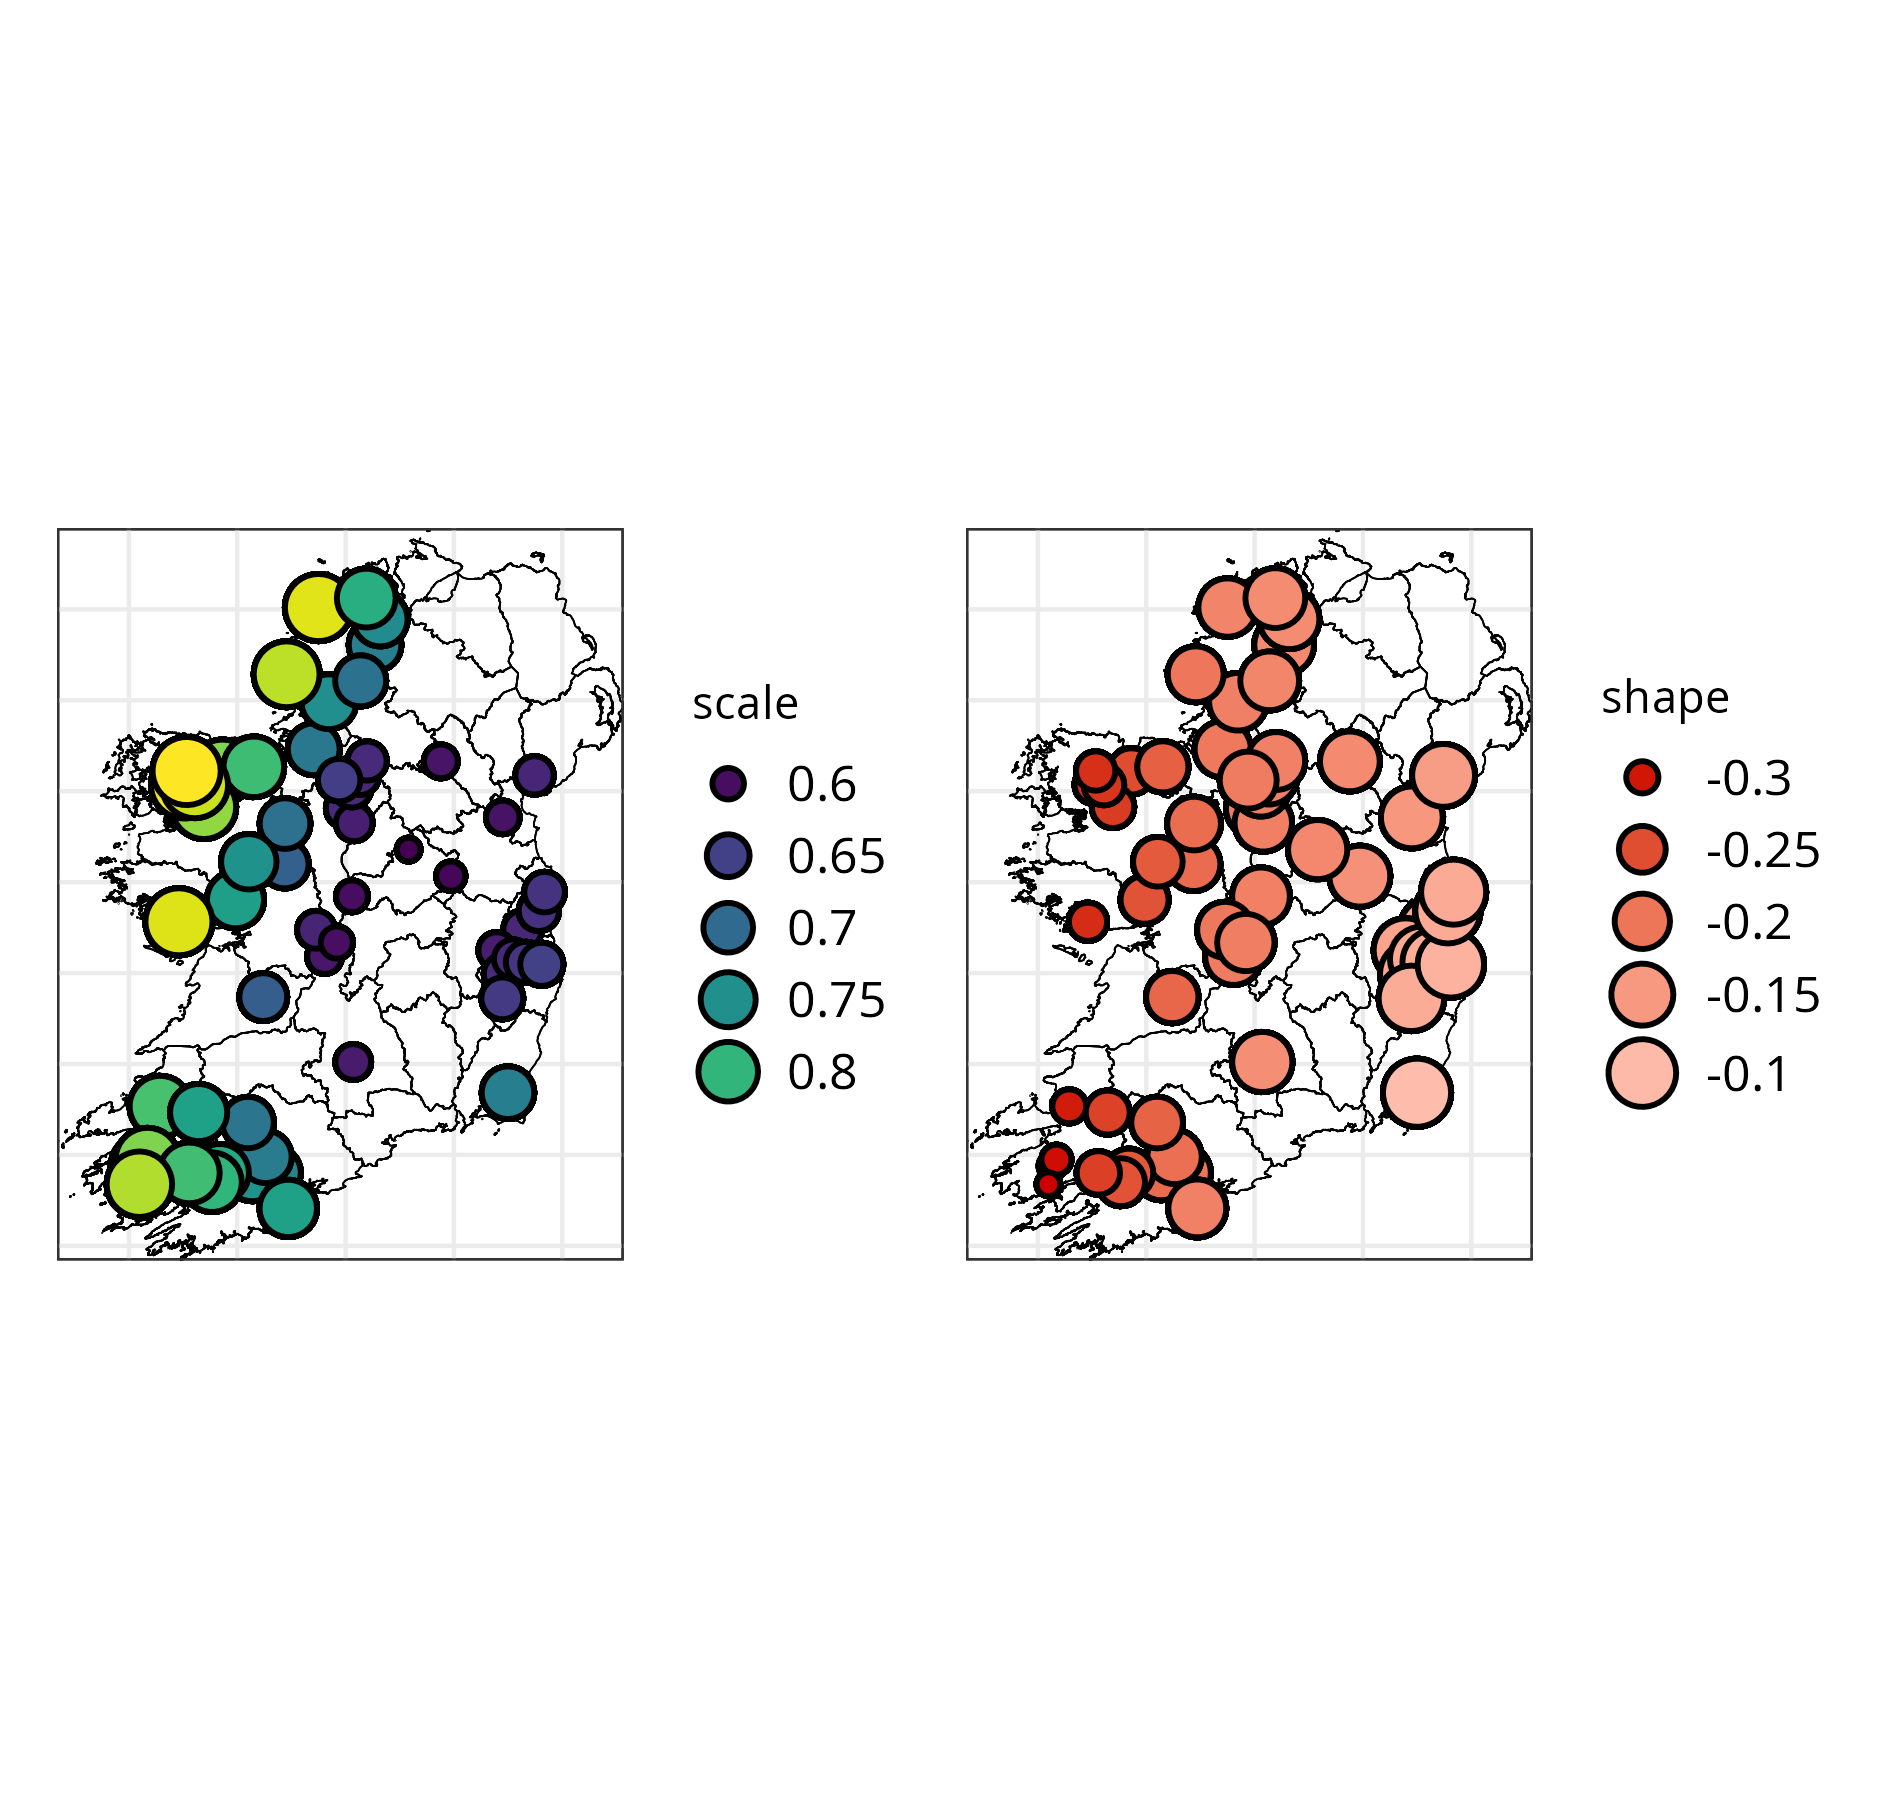
\includegraphics[width = 0.9\linewidth]{plots/033_gpd_ws.png}
    \caption{\emph{Figures, from left to right, showing the scale ($\sigma_wind)$ and shape ($\xi_wind$) parameters of the Generalised Pareto distribution for weekly wind speed maxima at each Met Éireann weather station.}}
    \label{fig:03_gpd_ws}
\end{figure}

% Also map of finite end points for wind speed, since it's difficult to interpret
\begin{figure}[H]
    \centering
    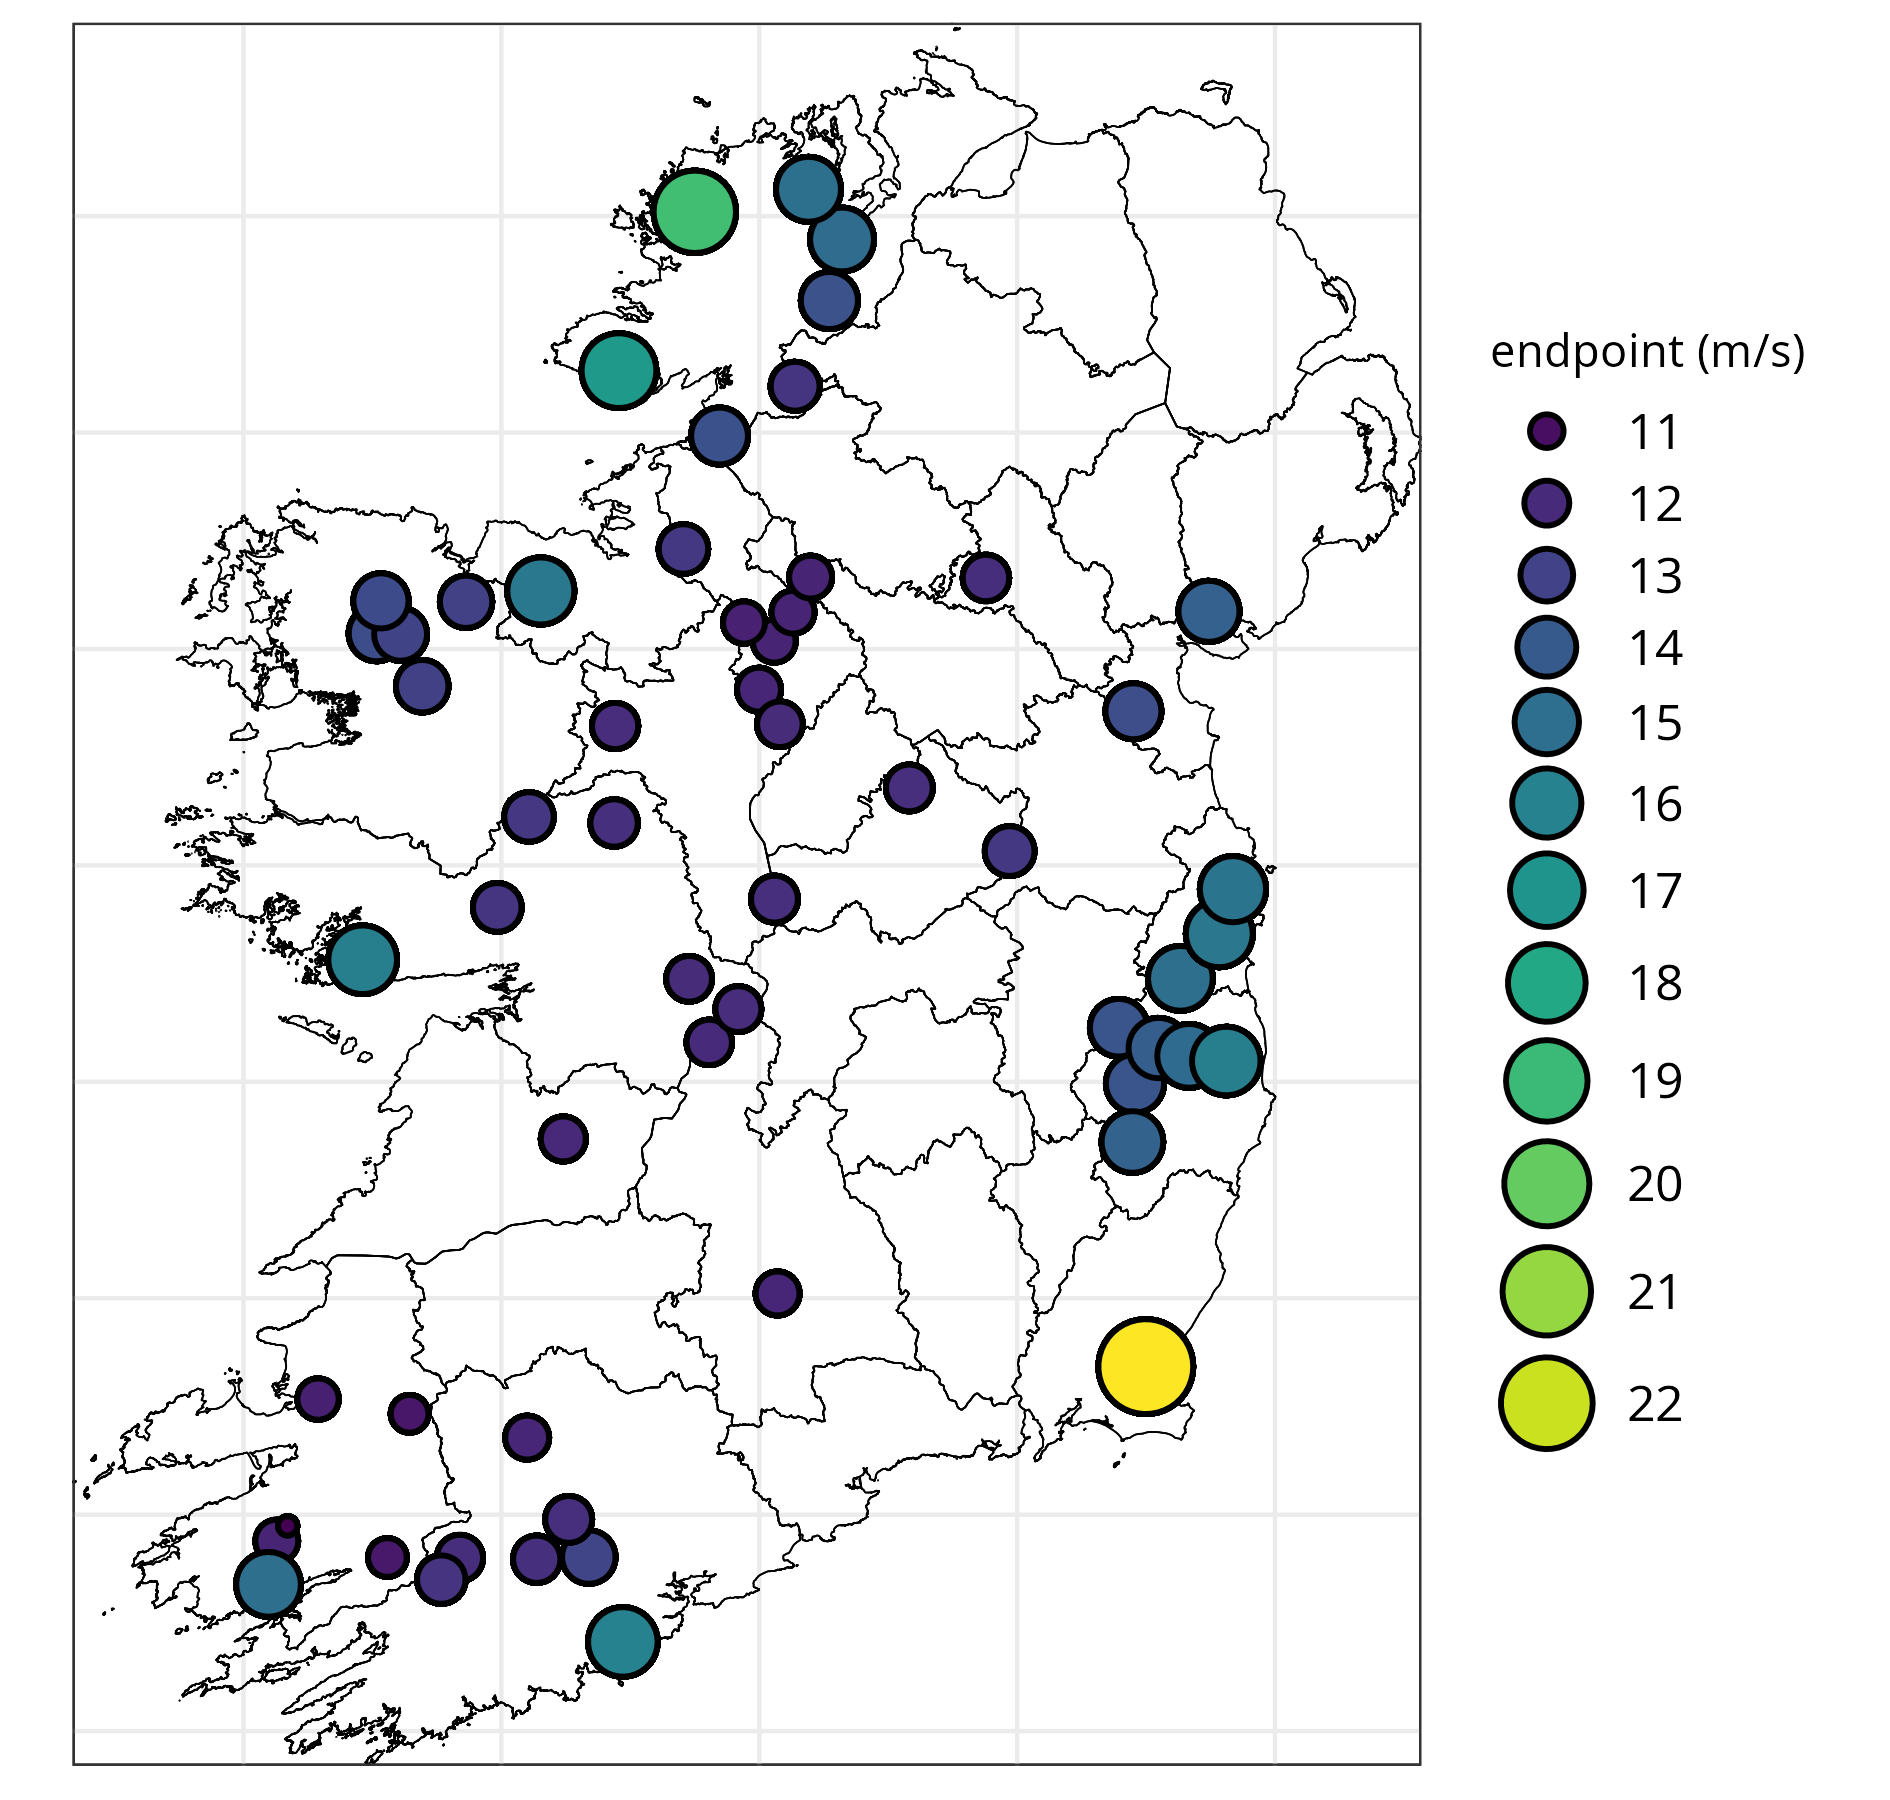
\includegraphics[width = 0.9\linewidth]{plots/034_ws_endpoint.png}
    \caption{\emph{Upper endpoints for Generalised Pareto Distribution fit for weekly wind speed maxima at each Met Éireann weather station.}}
    \label{fig:03_ws_endpoint}
\end{figure}

% comment on dynamics

% QQ, PP plots for GPD fits (with uncertainty)
\todo{Add back in labels, too difficult to understand}
\begin{figure}[H]
    \centering
    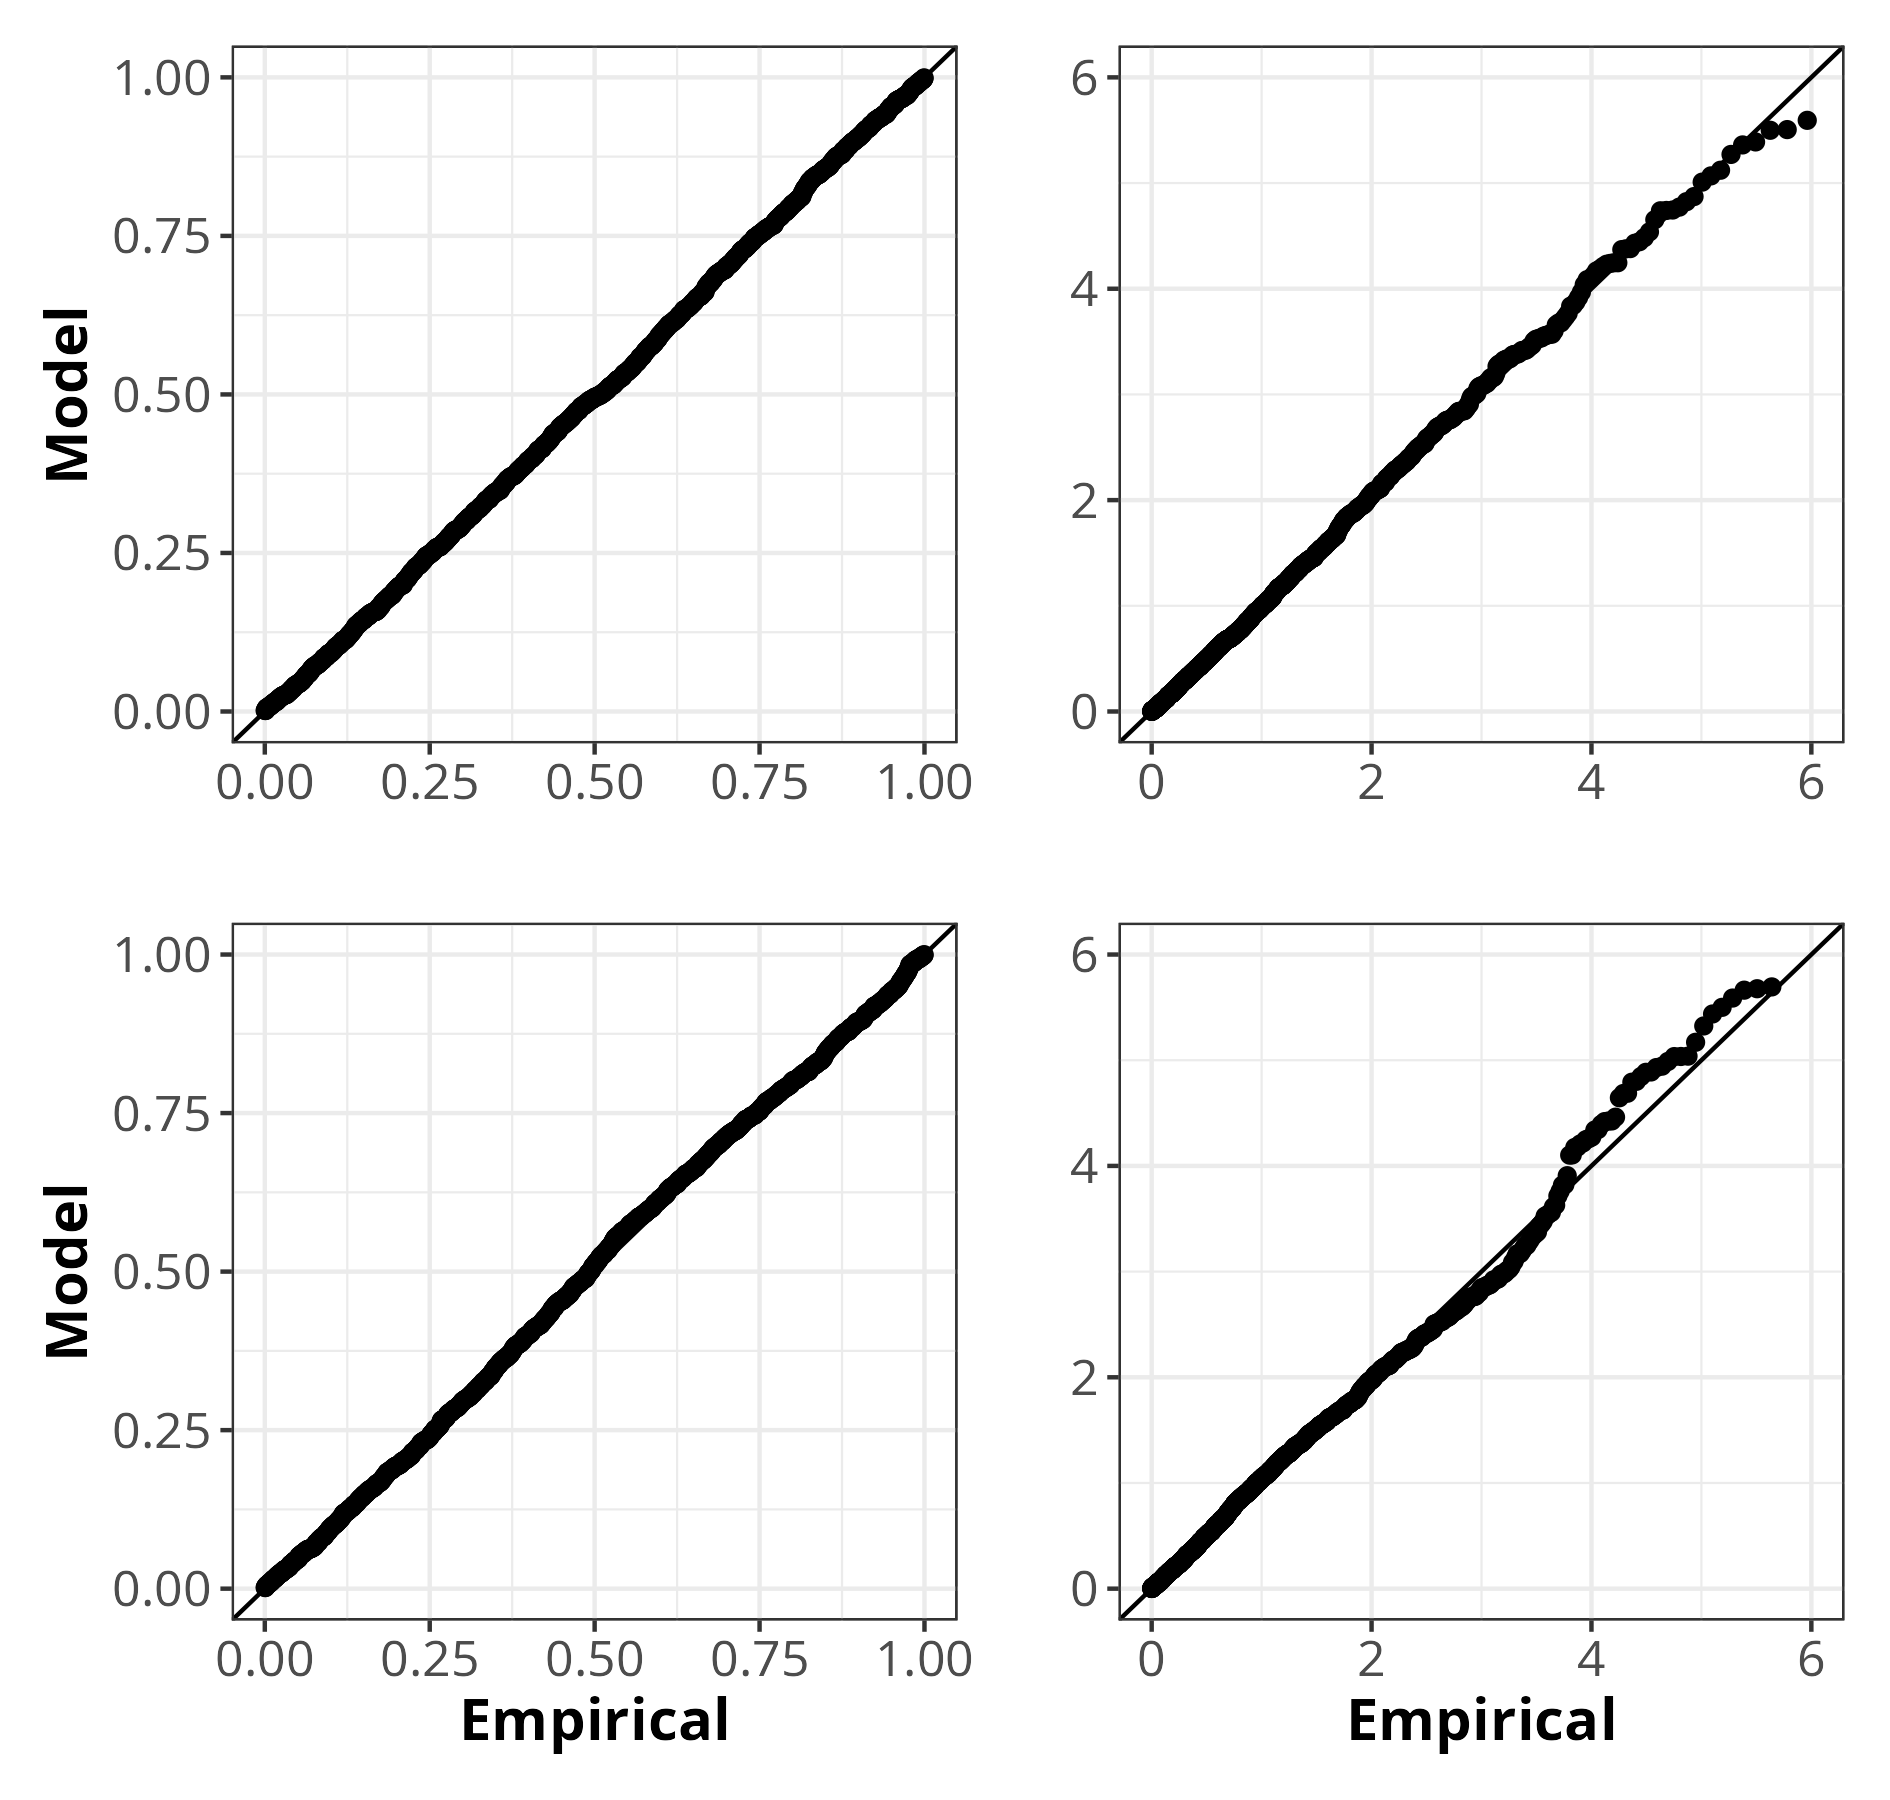
\includegraphics[width = 0.9\linewidth]{plots/035_pp_qq.png}
    % \caption{\emph{Test}}
    \caption{\emph{Figures in the first row shows the probability and quantile plots associated with the Generalised Pareto Distribution (GPD) fit to weekly total precipitation, while the second row shows the same plots for the GPD fit to weekly wind speed maxima.}}
    \label{fig:03_pp_qq}
\end{figure}

% Lead into dependence modelling

\newpage
\section{Conditional extremes}\label{sec:ce}

% Below narrative is a bit jumbled, can order better by looking at \cite{Heffernan2004}, \cite{Keef2013} and applied conditional extremes papers again. 
% \todo{Anything else to add?}
% \todo{Where to include applications? At the start?}
% \todo{Add section similar to univariate introducing the CE model}

% \begin{itemize}
%   \item Briefly motivate the need for dependence modelling
%   \item Describe dependence modelling more generally
%   \item Introduce the conditional extremes model for extremal dependence
%   \item Briefly describe extensions
%   \item apply to motivating example
% \end{itemize}

% While section \ref{sec:uni} introduced how the GPD can be fit to extreme data in a univariate or marginal context, we are often interested in modelling the dependence between extremes of different variables or at different locations.
As opposed to the univariate case, where we are interested in modelling the distribution of a single variable, we are often interested in modelling the dependence between extremes of different variables or at different locations.
For example, we may be interested in modelling the joint probability of extreme precipitation and wind speed at a given location, which may together produce especially damaging storm events.
In the context of the insurance and risk industries, these events are of particular interest, as they can lead to large payouts and significant losses.
Similarly, we may also be interested in the joint probability of extreme precipitation at different locations, which may lead to widespread flooding for which flood defences need to be coordinated and prepared.
Furthermore, in \cite{Zhang2024}, return level calculations have been shown to be improved by incorporating extremal dependence.
% We will focus on the former example in our motivating example.

% \todo{Rewrite from Heffernan2004}
\todo{Need to be more formal here, as in Heffernan2004?}
Formally, following the illustration in \cite{Heffernan2004}, suppose we have a continuous vector variable $\bm{X} = (X_1, X_2, \ldots, X_d)$, where each $X_i$ corresponds to a different marginal variable or location.
We want to estimate the joint probability $\mathbb{P}(\bm{X} \in \bm{C})$, where $\bm{C}$ is the set of extreme values for $\bm{X}$.
This probability can be decomposed as
\begin{equation} \label{eq:decomp}
  % \mathbb{P}(\bm{X} \in \bm{C}) = \sum_{i=1}^{d}{\mathbb{P}(\bm{X} \in C_i)} = \sum_{i=1}^{d}{\mathbb{P}(\bm{X} \in C_i \mid X_i > u_{X_i}) \mathbb{P}(X_i > u_{X_i})},
  \mathbb{P}(\bm{X} \in \bm{C}) = \sum_{i=1}^{d}{\mathbb{P}(\bm{X} \in C_i)} = \sum_{i=1}^{d}{\mathbb{P}(\bm{X} \in C_i \mid X_i > v_{X_i}) \mathbb{P}(X_i > v_{X_i})},
\end{equation}
where $v_{X_i} = \inf_{\bm{x} \in C_i}(x_i)$.
% where $u_{X_i}$ is the threshold for the $i^{th}$ component of $\bm{X}$.
The second of these probabilities can be estimated using a univariate GPD as in section \ref{sec:uni}, but the first requires a model for the dependence structure between the components of $\bm{X}$.

In this section, we will first introduce the concept of dependence modelling for extremes more generally, and then describe the conditional extremes model, a flexible model for extremal dependence which conditions on each variable in $\bm{X}$ to estimate its dependence structure, and how it can be fit to data and subsequently interpreted.
% The conditional extremes model is a more flexible and computationally feasible dependence model for extremes than its alternatives, such as max-stable processes, Pareto processes, Gaussian processes, and copulas \cite{Heffernan2004} \cite{Tawn2018} \cite{Huser2024}.
\todo{Add above to below section on CE model}
We will then briefly talk about some extensions to the original conditional extremes model of \cite{Heffernan2004} and the widely adopted revisions made in \cite{Keef2013}, before applying the model to our motivating example.

\subsection{Extremal Dependence}
\todo{Return to this section, also look at Keef 2013 for anything additional to add}
\todo{Could be made more clear? Why is chi bar between -1 and 1 for asymptotic independence}

In order to characterise the dependence between extremes, we must introduce the concepts of asymptotic dependence and independence, as described in \citet{Coles1999}.
% The coefficient of asymptotic dependence, $\chi \in [0, 1]$, measures the degree of asymptotic dependence between two random variables $X_1$ and $X_2$ with corresponding CDFs $F_1$ and $F_2$, under the class of asymptotically dependent distributions.
The coefficient of dependence, $\chi \in [0, 1]$, measures the degree of extremal dependence between two random variables $X_1$ and $X_2$ with corresponding CDFs $F_1$ and $F_2$, under the class of asymptotically dependent distributions.
It is defined as $\chi = \lim_{u \rightarrow 1}{\chi(u)}$, where
\[
  \chi(u) = \mathbb{P}\left( F_1(X_1) > u \mid F_2(X_2) > u \right), u \in [0, 1].
\]
If $\chi = 0$, then $X_1$ and $X_2$ are said to be asymptotically independent, while for $\chi > 0$, they are asymptotically dependent, with greater magnitude as $\chi$ increases \cite{Coles1999}.
Thus, $\chi$ gives the limit probability of $X_1$ being extreme given that $X_2$ is extreme, and we expect the joint probability of observing extremal events in both variables to be greater where $\chi$ is higher \cite{Rohrbeck2021}.
Furthermore, $\chi$ is symmetric in $X_1$ and $X_2$.
Two variables can be asymptotically dependent even if they are not dependent in the classical sense.
% Another coefficient, $\bar{\chi} \in [-1, 1]$, is used to measure the strength of dependence in the case of asymptotically independent distributions, where $\chi = 0$.
Another coefficient, $\bar{\chi} \in [-1, 1]$, is used to measure the strength of extremal dependence where $\chi = 0$, in the case of asymptotically independent distributions.
This coefficient is defined as $\bar{\chi} = \lim_{u \rightarrow 1}{\bar{\chi}(u)}$, where
\[
  \bar{\chi}(u) = \lim_{u \rightarrow 1} \frac{2\log\mathbb{P}(F_1(X_1) > u)}{ \log{\mathbb{P}(F_1(X_1) > u, F_2(X_2) > u)}} - 1.
\]
For asymptotic dependence, $\bar{\chi} = 1$.
Under asymptotic independence, $\bar{\chi} = 0$, with $\bar{\chi}$ increasing in magnitude as the variables become more positively (for $\bar{\chi} > 0$) or negatively (for $\bar{\chi} < 0$) dependent in their extremes \cite{Vignotto2021}.


Together, $(\chi, \bar{\chi})$ provide a useful summary of extremal dependence for any pair of random variables.
However, they are restricted to the bivariate setting, and they do not fully describe the dependence structure of a multivariate distribution.
For example, probabilities of jointly extreme events for two or more variables cannot be calculated from these coefficients.
For this, we require a model for extremal dependence.
Various approaches to this problem have included max-stable processes, Pareto processes, Gaussian processes and copulas.
However, these models are limited in their ability to model dependence and their computational feasibility, and are often conceptually quite difficult. 
For example, max-stable processes can only model $\mathbb{P}(\bm{X} \in \bm{C})$ under asymptotic dependence between each pair of variables in $\bm{X}$, while in contrast Gaussian processes can only model asymptotic independence \citep{Tawn2018, Huser2024}.
Max-stable processes are also quite computationally expensive and conceptually difficult to derive, and so are often not feasible for large datasets.
A model which provides a more flexible approach to modelling extremal dependence is the conditional extremes model of \cite{Heffernan2004}.

% Vignotto point
% Note that in this latter case, not all the considered variables need to lay in the tail region since the only one explicitly modeled as extreme is the conditioning variable (
% Heffernan and Tawn, 2004
% ). 

\subsection{Conditional extremes model}

\todo{Might be useful to include explanation of notation used in this section}
\todo{Include brief lit review of uses of CE model in various papers}

The conditional extremes model combines a piecewise semi-parametric marginal extremes model which includes a fitted GPD as described in section \ref{sec:uni} with a semi-parametric regression model for the dependence structure. 
It is seeing increasing use in the literature.
The model was first introduced in \citep{Heffernan2004}, where it was applied in the context of air pollutants, specifically modelling the dependence between $O_3$ and various sulphur- and nitrogen-based pollutants, for which $O_3$ is known to have synergistic corrosive effects. \todo{Rewrite from Heffernan2004}
In \citep{Keef2012_flooding}, the conditional extremes model was used to simulate a set of flood events in order to estimate the probability of widespread flooding. \todo{Rewrite from Keef2012}
\citep{Jonathan2013} models the joint probabilities of significant wave height and spectral peak period during peak oceanic storm events, which are important for the design of offshore structures. 
The severe heatwave experienced by Australia in 2009 was explored in \citep{Winter2016} using the model, to better understand the relationship between the El Niño-Southern oscillation and extreme temperature.
Some more recent extensions of the conditional extremes model which extend its feasibility in a variety of settings is discussed in section \ref{subsec:extensions}.

In this section, we describe the conditional extremes model, much as we did for the univariate GPD in section \ref{sec:uni}.

\subsubsection{Marginal model}
%   marginal model is piecewise ECDF and GPD, which can be fitted using any method mentioned in \ref{sec:uni}. 

The conditional extremes model requires a marginal model for the complete marginal distribution of a random variable $X_i$.
Therefore, realisations above a high threshold $u_{X_i}$ are modelled using a GPD, while the empirical distribution function is used for observations below this threshold.
% For simplicity, we leave out the space covariate $s$ in this section, although in practice we model our GPD as in equation \ref{eq:gpd_cov}.
For simplicity of notation, we return here to the stationary version of the GPD, although in practice we model our GPD as in equation \eqref{eq:non_stationary_gpd}.
The marginal distribution of $X_i$ under the conditional extremes model is therefore characterised by the piecewise semi-parametric model
\begin{equation} \label{eq:piecewise_marg}
  \hat{F}_{X_i}(x) = \begin{cases}
    1 - \{ 1 - \tilde{F}_{X_i}(u_{X_i})\} \left\{1 + \xi_{i}(x - u_{X_i})/\sigma_i\right\}_{+}^{-1/\xi_{i}} & \text{if } x > u_{X_i} \\
    \tilde{F}_{X_i}(x) & \text{if } x \le u_{X_i},
  \end{cases}
\end{equation}
where $\tilde{F}_{X_i}$ is the empirical distribution function of $X_i$.
It is important to note that this marginal model can be fit using any of the methods outlined in section \ref{sec:uni}, including with the use of covariates to model the parameters of the GPD, as in section \ref{subsubsec:non_stationary}.
\todo{Define gam function above, say how we've used it to estimate this model}
From equation \ref{eq:piecewise_marg}, we can estimate the probability of $X_i$ exceeding the threshold $u_{X_i}$, handling the second part of equation \eqref{eq:decomp}. 

\subsubsection{Marginal transformation}
% Requires Gumbel transformation of margins to have exponential upper tail, but this gives complex form for $a$ for negative dependence, so instead following \cite{Keef2013} Laplace margins are used which have doubly exponential tails and thus have the conceptually simple $a_{\mid i} = \alpha_{\mid i}Y_{\mid i} , b = Y_{\mid i}^{\beta_{\mid i}}$, which can be interpreted as the slope and spread parameters for our semi-parametric regression line (is there a reference I can use which makes this interpretation?). 

\todo{Go through and check bm X vs X!}

The conditional extremes model requires the marginal distributions $\bm{X}_i$ to have an exponential upper tail, which greatly simplifies the estimation procedure for the dependence structure.
Furthermore, it is useful to have common marginal distributions, as we are interested in rare events in our margins regardless of their original scales, as in our example, where we compare extremal wind speed, measured in metres per second, and precipitation, measured in mm \cite{Winter2016}.
In \cite{Heffernan2004}, this is achieved by transforming the marginal distribution to a Gumbel distribution, which has an exponential upper tail.
% This transformation, for which we denote the transformed marginal variable as $Y_i$, is given by
% \begin{equation} \label{eq:gumbel}
%   Y_i = -\log[-\log\{\hat{F}_{X_i}(X_i)\}], i = 1, \ldots, d. \\
% \end{equation}
% This results in $\mathbb{P}(Y_i \le y) = \exp(-\exp(-y))$ and hence $\mathbb{P}(Y_i > y) \sim \exp(-y) \text{ as } y \rightarrow \infty$, so $Y_i$ has an exponential upper tail.  
% However, this results in a relatively complex form for the normalising functions in the semi-parametric regression model for the dependence structure in the case of negative dependence, since the lower tail of the Gumbel distribution is not exponential.
However, this results in a relatively complex form of the model in the case of negative dependence, since the lower tail of the Gumbel distribution is not exponential.
% This topic is treated in more detail in section \ref{subsubsec:ce_normalisation}.

A much more common approach, first proposed in \cite{Keef2013}, is to instead use a Laplace transformation, which has a doubly exponential tails.
This transformation, which we denote as $Y_i$ to differentiate from the marginals $\bm{X}$ on their original scales, is given by 
\begin{equation} \label{eq:laplace}
  Y_i = \begin{cases}
    % \exp(y)/2 &\text{ for } y < 0 \\
    \log\left\{2F_{X_i}(X_i)\right\} &\text{ for } X_i < F_{X_i}^{-1}(0.5), \\
    -\log\left\{2(1 - F_{X_i}(X_i))\right\} &\text{ for } X_i \ge F_{X_i}^{-1}(0.5), \\
  \end{cases}
\end{equation}
% \begin{equation} \label{eq:laplace_tails}
%   \mathbb{P}(Y_i \le y) = \begin{cases}
%     \exp(y)/2 &\text{ for } y < 0 \\
%     1-\exp(-y)/2 &\text{ for } y \ge 0. \\
%   \end{cases}
% \end{equation}
Both tails of $Y_i$ are exponential, and for any $u > 0$, the distribution of $Y_i - u \mid Y_i > u$ and $(-Y_i + u) \mid Y_i \le -u$ are exponential with mean 1. 
This greatly simplifies the normalising functions, as the form of $a_{\mid i}$ is the same for both positive and negative dependence. 

After this transformation, we are left with a vector of transformed variables $\bm{Y}$ with common Laplace margins. 

\subsubsection{Asymptotic motivation}
% Starting from asymptotic motivation, define conditional extremes model as in \cite{Heffernan2004} and in applied paper as the non-parametric regression equation $Y_{-i} = a_{\mid i}(Y_{\mid i}) + \b_{\mid i}(Y_{\mid i}) Z_{\mid i}$

Vector algebra in this section and throughout is to be interpreted as componentwise.
Here and below, we use $Y_{-i} = {\bm{Y}_1, \ldots, \bm{Y}_{i-1}, \bm{Y}_{i+1}, \ldots, \bm{Y}_d}$ to denote the vector $\bm{Y}$ with the $i^{th}$ component removed. \todo{never mentioned d? or defined how many vectors I will have?}
Furthermore, we use the notation $\bm{a}_{\mid i}$ to denote the vector normalising function conditional on $Y_i$, and $a_{j \mid i}$ to denote the value of $\bm{a}_{\mid i}$ associated with $Y_j$, for some $j \ne i$. 
\todo{Word better}
\todo{May need to move this to the start of the section? Or have a glossary at the start of the report?}
\todo{relate to motivating example?}

\todo{Need to mention how this is an assumption}
\todo{Rewrite more in own words}
Following a similar line of reasoning to the univariate asymptotic motivation detailed in section \ref{subsubsec:asymptotic}, for each $Y_i$, we want to estimate $\lim_{y \to \infty}\{\mathbb{P}(\bm{Y}_{-i} \le \bm{y}_{-i} \mid Y_i = y_i)\}$. 
Therefore, we require the limiting distribution to be non-degenerate for all margins.
% This is achieved by the principal assumption of the conditional extremes model, mirroring that in equation \ref{eq:uni_limiting_dist} for univariate extremes, which is that for each $i$, there exists vector normalising functions $\bm{a}_{\mid i}(y_i),\bm{b}_{\mid i}(y_i), \in \mathbb{R} \rightarrow \mathbb{R}^{(d-1)}$ such that for fixed $\bm{z}_{\mid i}$,
This is achieved by the principal assumption of the conditional extremes model that for each $i$, there exists vector normalising functions $\bm{a}_{\mid i}(y_i),\bm{b}_{\mid i}(y_i), \in \mathbb{R} \rightarrow \mathbb{R}^{(d-1)}$ such that for fixed $\bm{z}_{\mid i}$,
\begin{equation} \label{eq:ce_limiting_dist}
      \lim_{y_i \rightarrow \infty}\{\mathbb{P}(\bm{Y}_{-i} \le \bm{a}_{\mid i}(y_i) + \bm{b}_{\mid i}(y_i)\bm{z}_{\mid i} \mid Y_i = y_i)\} = \bm{G}_{\mid i}(\bm{z}_{\mid i}),
\end{equation}
where $G_{j \mid i}$ is non-degenerate for all $j \ne i$. 
\todo{Ensure we have bm G throughout}
Furthermore, to ensure $\bm{G}_{\mid i}$ is well-defined, we must have the constraint that 
\[
  \lim_{z \rightarrow \infty}{\bm{G}_{j \mid i}(\bm{z})} = 1, \forall j \ne i,
\]
ensuring that there is no mass at $+\infty$ for any margin, but allowing for some mass to be at $-\infty$ \cite{Keef2013}. \todo{Why is this}

An alternative formulation of the assumption in equation \ref{eq:ce_limiting_dist} which can be more readily adapted into our dependence model in section \ref{subsubsec:dep_model} is
\begin{equation} \label{eq:standardised_residuals}
  \bm{Z}_{\mid i} = \frac{\bm{Y}_{-i} - \bm{a}_{\mid i}(y_i)} {\bm{b}_{\mid i}(y_i)},
\end{equation}
where $\bm{Z}_{\mid i}$ is the vector of standardised residuals for our model, and again following our univariate argument in section \ref{subsubsec:asymptotic}, we have that
\[
      \lim_{y_i \rightarrow \infty}\{\mathbb{P}(\bm{Z}_{\mid i} \le \bm{z}_{\mid i} \mid Y_i = y_i)\} = \bm{G}_{\mid i}(\bm{z}_{\mid i})
\]

An important consequence of this formulation is the weak assumption that
\begin{equation} \label{eq:limit_independence}
\mathbb{P}(\bm{Z}_{\mid i} \le \bm{z}_{\mid i}, Y_i - u_i = y_i \mid Y_i > u_i) \rightarrow G_{\mid i}(\bm{z}_i) \exp(-y) \text{ as } u_i \rightarrow \infty,
\end{equation}
so that in the limit as $u_i \to \infty$, the extremal exceedances $Y_i - u_i$ and $\bm{Z}_{\mid i}$ are independent.
Methods for assessing the validity of this assumption and hence the conditional extremes model for a given application are explored in section \ref{subsubsec:ce_diagnostics}.


\subsubsection{Dependence model} \label{subsubsec:dep_model}

\todo{Perhaps (here or below) mention how G estimated nonparametrically, for Z hat on page 508?}
\todo{Also, is there a need to explicitely define the model for Z j mid i (page 504)?}
\todo{Need to say somewhere how in practice, Z is first sampled from a normal distribution and thereafter empirically estimated, see inference section in Keef}

% \subsubsection{Normalisation} \label{subsubsec:ce_normalisation}


% \todo{Shooter 2020 has good interpretation of normalising functions}

% Under Gumbel margins, the normalising functions are given by:
% \begin{align} \label{eq:gumbel_normalisation}
%   \begin{split}
%     \bm{a}_{\mid i}(y) &= \bm{\alpha}_i y + I_{\{\bm{\alpha}_{\mid i} = 0, \bm{\beta}_{\mid i} < 0\}} \{\bm{\gamma}_{\mid i} - \bm{\delta}_{\mid i}\log(y)\}, \\
%     \bm{b}_{\mid i}(y) &= y^{\bm{\beta}_{\mid i}}, 
%   \end{split}
%  \end{align}
% where $\ldots$ \todo{Define constants above, say how alpha and beta in indicator function refer to negative dependence}
% Hence, they have quite a simple form for the class of positively associated variables, as the Gumbel margins have exponential upper tails for which the indicator function will equal zero, but a more complex and difficult to interpret formulation for negatively associated variables, as no such thing can be said about their lower tails. 

Under the Laplace marginal transformation in \citet{Keef2013}, we have doubly exponential tailed margins, and thus have the same form of normalising functions for both positive and negative dependence.

Specifically, the normalising functions are given by
\begin{align} \label{eq:laplace_normalisation}
  \begin{split}
    \bm{a}_{\mid i}(y) &= \bm{\alpha}_i y, \\
    \bm{b}_{\mid i}(y) &= y^{\bm{\beta}_{\mid i}}, 
  \end{split}
\end{align}
% where $\bm{\alpha}_{\mid i} \in [-1, 1], \bm{\beta}_{\mid i} \in \(-\infty, 1)$. 
where $(\bm{\alpha}_{\mid i}, \bm{\beta}_{\mid i}) \in [-1, 1]^{d-1} \times (-\infty, 1)^{d-1}$. % \citep{Keef2013}. \todo{Go back over citations throughout!}
% The interpretation of $\bm{\alpha}_{\mid i}$ and $\bm{\beta}_{\mid i}$ is discussed in greater detail in the next section in relation to the regression model for the dependence structure.
Rearranging equation \ref{eq:standardised_residuals} for our standardised residuals, and imputing the values for the vector normalising functions $\bm{a}_{\mid i}$ and $\bm{b}_{\mid i}$ from equation \ref{eq:laplace_normalisation}, we can now define the dependence model used in the conditional extremes model, which takes the form of the multivariate semi-parametric regression equation
\begin{align} \label{eq:ce_model}
  \begin{split}
    \bm{Y}_{-i} &= \bm{a}_{\mid i}(\bm{y}_i) + \bm{b}_{\mid i}(\bm{y}_i)\bm{Z}_{\mid i} \\
                &= \bm{\alpha}_{\mid i}\bm{y}_i + \bm{y}_i^{\bm{\beta}_{\mid i}}\bm{Z}_{\mid i}, \text{ for } Y_i = y_i > u_{Y_i}.
  \end{split}
\end{align}
\todo{Perhaps change to more clear formulation in Shooter2020?}
The normalising functions $\bm{a}_{\mid i}$ and $\bm{b}_{\mid i}$ can be interpreted as the slope and spread parameters for our semi-parametric regression line.
The level of association between $\bm{Y}_{-i}$ (i.e.\ each $Y_j, j \ne i$) and large $Y_i$ is controlled by $\bm{\alpha}_{\mid i}$, with positive and negative values indicating positive and negative dependence, respectively, and values closer to 0 indicating stronger independence.
The impact of the residual term $\bm{Z}_{\mid i}$ on the dependence between $\bm{Y}_{-i}$ and $\bm{Y}_i$ is controlled by $\bm{\beta}_{\mid i}$.
Lower values of $\bm{\beta}_{\mid i}$ indicate a more strongly deterministic relationship between $\bm{Y}_{-i}$ and $\bm{Y}_i$, while higher values indicate a more stochastic relationship \citep{Winter2016}.

Several special cases arise for certain values of $\bm{\alpha}_{\mid i}$ and $\bm{\beta}_{\mid i}$.
For example, when $\bm{\alpha}_{\mid i} = 0$ and $\bm{\beta}_{\mid i} = 0$, then $\bm{Y}_{-i}$ and $\bm{Y}_i$ are independent.
For $\bm{\beta}_{\mid i} = 0$, asymptotic positive and negative dependence are indicated by $\bm{\alpha}_{\mid i} = 1$ and $\bm{\alpha}_{\mid i} = -1$, respectively.
For the values $-1 < \bm{\alpha}_{\mid i} < 1$, $\bm{Y}_{-i}$ and $\bm{Y}_i$ are asymptotically independent.

\todo{Need to look into differences between independence and asymptotic independence!}
\todo{Add equation for Y j mid i? Perhaps somewhat clearer notation}
% \todo{Add special cases (asymptotic dependence, asymptotic independence?)}

% Additional constraints
% \todo{texmex vignette has good description of this}
In \citet{Keef2013}, additional constraints are placed on the possible values of $\bm{\alpha}_{\mid i}$ and $\bm{\beta}_{\mid i}$.
These constraints serve to enforce consistency of the fitted dependence model with the extremal dependence of the data \citep{Southworth2024_vignette}.

\subsubsection{Estimation} \label{subsubsec:estimation}
% How model is estimated, assuming normal dist for Z, then empirical dist
\todo{See Winter2016 for good description}
\todo{Come back to this!}

The estimation of the conditional extremes model has seen several developments since its introduction in \cite{Heffernan2004}.
Inference begins by first generating $Z_{\mid i}$ from a mutually independent multivariate normal distribution with some mean vector $\mu_{\mid i}$ and standard deviation $\sigma_{\mid i}$, i.e.\ $Z_{\mid i} \sim N(\mu_{\mid i}, \sigma_{\mid i})$. 
This initial form for $G_{\mid i}$, the distribution of $Z_{\mid i}$, was chosen experimentally. 
% Then, returning to equation \ref{eq:ce_model}, the conditional distribution $\bm{Y}_{\mid i} \mid Y_i$ for $Y_i > u$ is also multivariate normal so tha
Then, returning to equation \eqref{eq:ce_model}, the conditional distribution also follows a multivariate normal distribution, with
\[
  \bm{Y}_{-i} \mid \bm{Y}_i = y_i \sim N\left(\bm{\alpha}_{\mid i} y_i + y_i^{\bm{\beta}_i} \bm{\mu}_{\mid i}, y_i^{\bm{\beta}_i} \bm{\sigma_{\mid i}}\right),
\]
for $Y_i > u$. \todo{Is conditioning/notation right here??}
With this formulation, we can use likelihood methods to estimate the parameters $\hat{\bm{\alpha}}_{\mid i}$ and $\hat{\bm{\beta}}_{\mid i}$, as well as the nuisance parameters $\hat{\bm{\mu}}_{\mid i}$ and $\hat{\bm{\sigma}}_{\mid i}$.
Finally, we now nonparametrically estimate $G_{\mid i}$ as the empirical distribution of 
\[
  \bm{Z}_{\mid i} = \frac{\bm{Y}_{-i} - \hat{\bm{\alpha}}_{\mid i}Y_i}{Y_i^{\hat{\bm{\beta}}_{\mid i}}}.
\]

One of the benefits of the conditional extremes model is the ease with which Monte Carlo (MC) samples can be generated from the fitted model.
These samples can be used to calculate the probability of $\bm{X} \in \bm{C}$ conditioning on various $X_{\mid i}$, and return levels can be calculated as high quantiles of these simulations.
Many different MC algorithms have been proposed for this purpose, including the one described in \cite{Heffernan2004} and an alternative rejection sampling method in \cite{Keef2012_flooding}.
\todo{Need to describe algorithm in detail?}

% We will follow the procedure described in \cite{Winter2016} \todo{Will we?}
% First, we assume the standardised residuals $\bm{Z}_{\mid i}$ are normally distributed, and sample them from a multivariate normal distribution $\ldots$.
% Afterwards, we discard this assumption and estimate 
% We then estimate the normalising functions $\bm{\alpha}_{\mid i}$ and $\bm{\beta}_{\mid i}$ by fitting a non-parametric regression model to the data.

% The generally followed procedure is to first sample the standardised residuals $\bm{Z}_{\mid i}$ from a multivariate normal distribution, and then estimate the normalising functions $\bm{\alpha}_{\mid i}$ and $\bm{\beta}_{\mid i}$ by fitting a non-parametric regression model to the data.

\todo{Refer to extrapolation procedure, how easy it is generate MC sample from CE, return levels can be calculated as high quantiles of these simulations}

% \subsubsection{Extrapolation} \label{subsubsec:extrapolation}
% % Extrapolation through MC algorithm as in \cite{Heffernan2004} (alternative in \cite{Keef2013}.

% \todo{Change this algorithm from Heffernan to Keef}
% \todo{Also look at other Keef apper on flood events, seems to be most recent in that series}
% \todo{How do nu and u differ? Is it for thresholding X vs Y?}
% \begin{itemize}
  % \item Can simulate from $\bm{X}|\bm{X}_i > \nu_{X_i}$ by simulating from $\bm{Y}|\bm{Y}_i > y_i$ and transforming back to $\bm{X}$ space, using the following algorithm:
    % \begin{enumerate}
      % \item Simulate $Y_i$ from the transformed marginal distribution conditional on exceeding $t_i(\nu_{X_i})$.
      % \item Sample $\bm{Z}_{\mid i}$ from $\hat{G}_{\mid i}$, independently of $Y_i$. 
      % \item Obtain $\bm{Y}_{-i} = \bm{\alpha}_{\mid i}(Y_i) + (Y_i)^{\bm{\beta}_{\mid i}}\bm{Z}_{\mid i}$.
      % \item Transform $\bm{Y} = (\bm{Y}_{-i}, Y_i)$ back to the original scale by using the inverse of the marginal transformation. 
      % \item the resulting vector $\bm{X}$ is a simulated value from $\bm{X} \mid X_i > \nu_{X_i}$.
    % \end{enumerate}
  % \item This algorithm can be used to estimate $\mathbb{P}(\bm{X} \in C_i \mid X_i > \nu_{X_i})$ by evaluating it as the long run proportion of the generated sample that falls in $C_i$. 
% \end{itemize}

\subsubsection{Diagnostics} \label{subsubsec:ce_diagnostics}
% Talk about diagnostics through independence of residuals and tail exceedances in the limit. 

The marginal model is diagnosed as in univariate EVT, with threshold selection and model fit assessed through probability and quantile plots, as described in section \ref{subsubsec:uni_diagnostics}.

% \todo{Need to reference texmex vignette for this?}
% \todo{Talk about texmex here anyway, to make this theory more relative to its applications}
\todo{Check use of apostrophes}
For diagnosing the dependence model, we return to the weak assumption in equation \ref{eq:limit_independence} of asymptotic independence between the standardised residuals $\bm{Z}_{\mid i}$ and the exceedances $Y_i - u_i$, as $u_i \to \infty$.
The normalised residuals $\bm{Z}_{\mid i}$ must be stable across the range of $Y_i$ values over which they were estimated. 
Therefore, a plot of $Z_{\mid i}$ against $\hat{F}(Y_i)$ should show no trend, and the residuals should be approximately constant over the range of $Y_i$ values used for estimation.
\todo{F Y or F X? Does it matter?}
A number of statistical tests for independence can also be used, such as the corresponding test statistic of the Pearson correlation coefficient. 

Another graphical diagnostic tool is to overlay the fitted quantiles of the conditional extremes model on a plot of the raw data. 
This can be used to assess how well these quantiles agree with the shape of the data \citep{Southworth2024_vignette}.


\subsubsection{Uncertainty} \label{subsubsec:ce_uncertainty}

\todo{Come back to this!}

There are numerous sources of uncertainty intrinsic to the estimation of the conditional extremes model.
These include the shape and scale parameters of the marginal GPDs, the normalising functions in the dependence model and the standardised residuals. 
The uncertainty in each of these sources can be estimated using bootstrapping, as described in \citet{Heffernan2004}.
For fixed marginal and dependence thresholds, we can perform bootstrapping by resampling the residuals and the exceedances, and then refitting the marginal and dependence models to the resampled data.
We can also perform bootstrapping for different dependence thresholds as a means of choosing a threshold which gives the least uncertainty in the estimates of $\bm{\alpha}_{\mid i}$ and $\bm{\beta}_{\mid i}$ \citep{Southworth2024_vignette}.

\subsection{Extensions} \label{subsec:extensions}

There have been several extensions to the original conditional extremes model of \cite{Heffernan2004} and the additions of \cite{Keef2013}, particularly for the modelling of spatial and/or temporal extremes, which we will briefly cover below. 

\todo{Richards2023 (EVA challenge) has good summary of this}
\todo{Should I adopt minus notation for all CE models rather than mid i?}
In \cite{Winter2016}, the conditional extremes model is extended to include time-varying covariates for the normalising functions in the dependence model at each location, treating them as non-stationary.
Here, we use $\bm{\alpha}_{-s, t}$ and $\bm{\beta}_{-s, t}$ to denote the vectors $\bm{\alpha}_t$ and $\bm{\beta}_t$ corresponding to the vector $\bm{Y}_t$ without its $s$-th location, as using the $\bm{\alpha}_{\mid i}$ notation of section \ref{subsubsec:dep_model}
is rather ambiguous in this spatio-temporal context. \todo{Review this, what am I trying to say?}
% the parameters of the dependence model in equation \ref{eq:ce_model} at some location $s$ and time $t$ are modelled as functions of some time-varying covariates $g_t$ using the generalised linear models
Therefore, the normalising functions are themselves modelled as
\begin{align} \label{eq:ce_winter}
  \begin{split}
  % \bm{\alpha}_{\mid i}(s, t) &= \bm{\alpha}_{\mid i}(s) + \bm{\gamma}_{\mid i}g_t, \\
  \tanh^{-1}(\bm{\alpha}_{-s, t}) &= \bm{\alpha}^{(0)}_{-s} + \bm{\alpha}^{(1)}_{-s}g_t, \\
  \tanh^{-1}(\bm{\beta}_{-s, t}) &= \bm{\beta}^{(0)}_{-s} + \bm{\beta}^{(1)}_{-s}g_t,
  \end{split}
\end{align}
with intercept and slope parameters $\bm{\alpha}^{(0)}_{-s}, \bm{\alpha}^{(1)}_{-s}, \bm{\beta}^{(0)}_{-s}, \bm{\beta}^{(1)}_{-s} \in \mathbb{R}^{d-1}$ and temporal covariate $g_t$.
The inverse hyperbolic tangent function $\tanh^{-1}$ is used as a link function as it restricts the parameters to the range $[-1, 1]$. 
While $\beta$ within the conditional extremes model can theoretically range from $-\infty$ to 1, in practice $\beta$ is rarely seen to be less than $-1$, as this would result in an almost deterministic relationship with the conditioning variable, which is rarely realistic, so this link function is appropriate. 
In \cite{Richards2023}, the logit link function is instead used for $\bm{\beta}_{-s, t}$. 

% \todo{Write this section!}
\todo{Enough written for this section? Trying to keep somewhat vague}
\cite{Wadsworth2018} extends the conditional extremes model to a spatial context, where the dependence model is extended to include a spatially varying dependence structure within the normalising functions. 
The model represents $\alpha$ as a slowly decaying function of the distance between some reference site and the site in question.
Several choices of $\bm{\beta}_{-s}$ are considered to fit different tails, and the residuals are modelled as a Gaussian process with some constraints to ensure that the residuals are 0 when the site in question is the same as the reference site.
This model was further extended to the spatio-temporal case in \citet{Simpson2021}, adapting the dependence model to condition on a reference location in time as well as space. 

Despite these extensions, the conditional extremes model is still rather computationally expensive, and has its applications have been limited to datasets with hundreds of locations.
\cite{Simpson2023} further extends the feasibility of this model for large datasets with thousands of locations. 
By reformulating the spatial conditional extremes model slightly to fit into the class of latent Gaussian models, the model can be fit using INLA.
This has opened up the conditional extremes model to a wider range of applications, particularly in the context of high-dimensional spatio-temporal and geostatistical data.

\subsection{Application to motivating example} \label{subsec:ce_example}

(Not necessarily in correct order)
\begin{itemize}
  \item used \texttt{texmex} to fit conditional extremes model on top of marginal models to estimate $\alpha, \beta$ for rain $\mid$ wind speed and vice versa for each location. 
        Vanilla CE used for simplicity of implementation for this motivating example. 
   \begin{enumerate}
     \item Show diagnostic and quantile plots for CE for some location(s),
     \item Show bootstrapped $\alpha$ and $\beta$ values for rain $\mid$ wind speed and wind speed $\mid$ rain for different thresholds, motivating choice of CE threshold at 70th quantile, and fixing $\beta$ at 0.1 so that all variability is in $\alpha$ (also makes interpretation easier, and need for this further highlights need for better parameter estimation through grouping and/or some hierarchical model). 
     \item Bootstrapped values for $\xi$ (under vanilla \texttt{texmex} marginal estimates, rather than \texttt{evgam}) and $\alpha$ show that uncertainty high in both, even when fixing $\beta$. 
     \item Maps of $\alpha$ values conditioning on rain and windspeed, possibly cross-hatch where bootstrapped $\alpha$ values have 95\% CI which intersects 0. 
     \item Plot of $\alpha$ values versus longitude and latitude (possibly coloured by distance to coast), showing how space is main driver in difference (unsurprising as used as only covariate in marginal \texttt{evgam} model). 
   \end{enumerate}
\end{itemize}

% Plot of chi and chi bar
\begin{figure}[H]
    \centering
    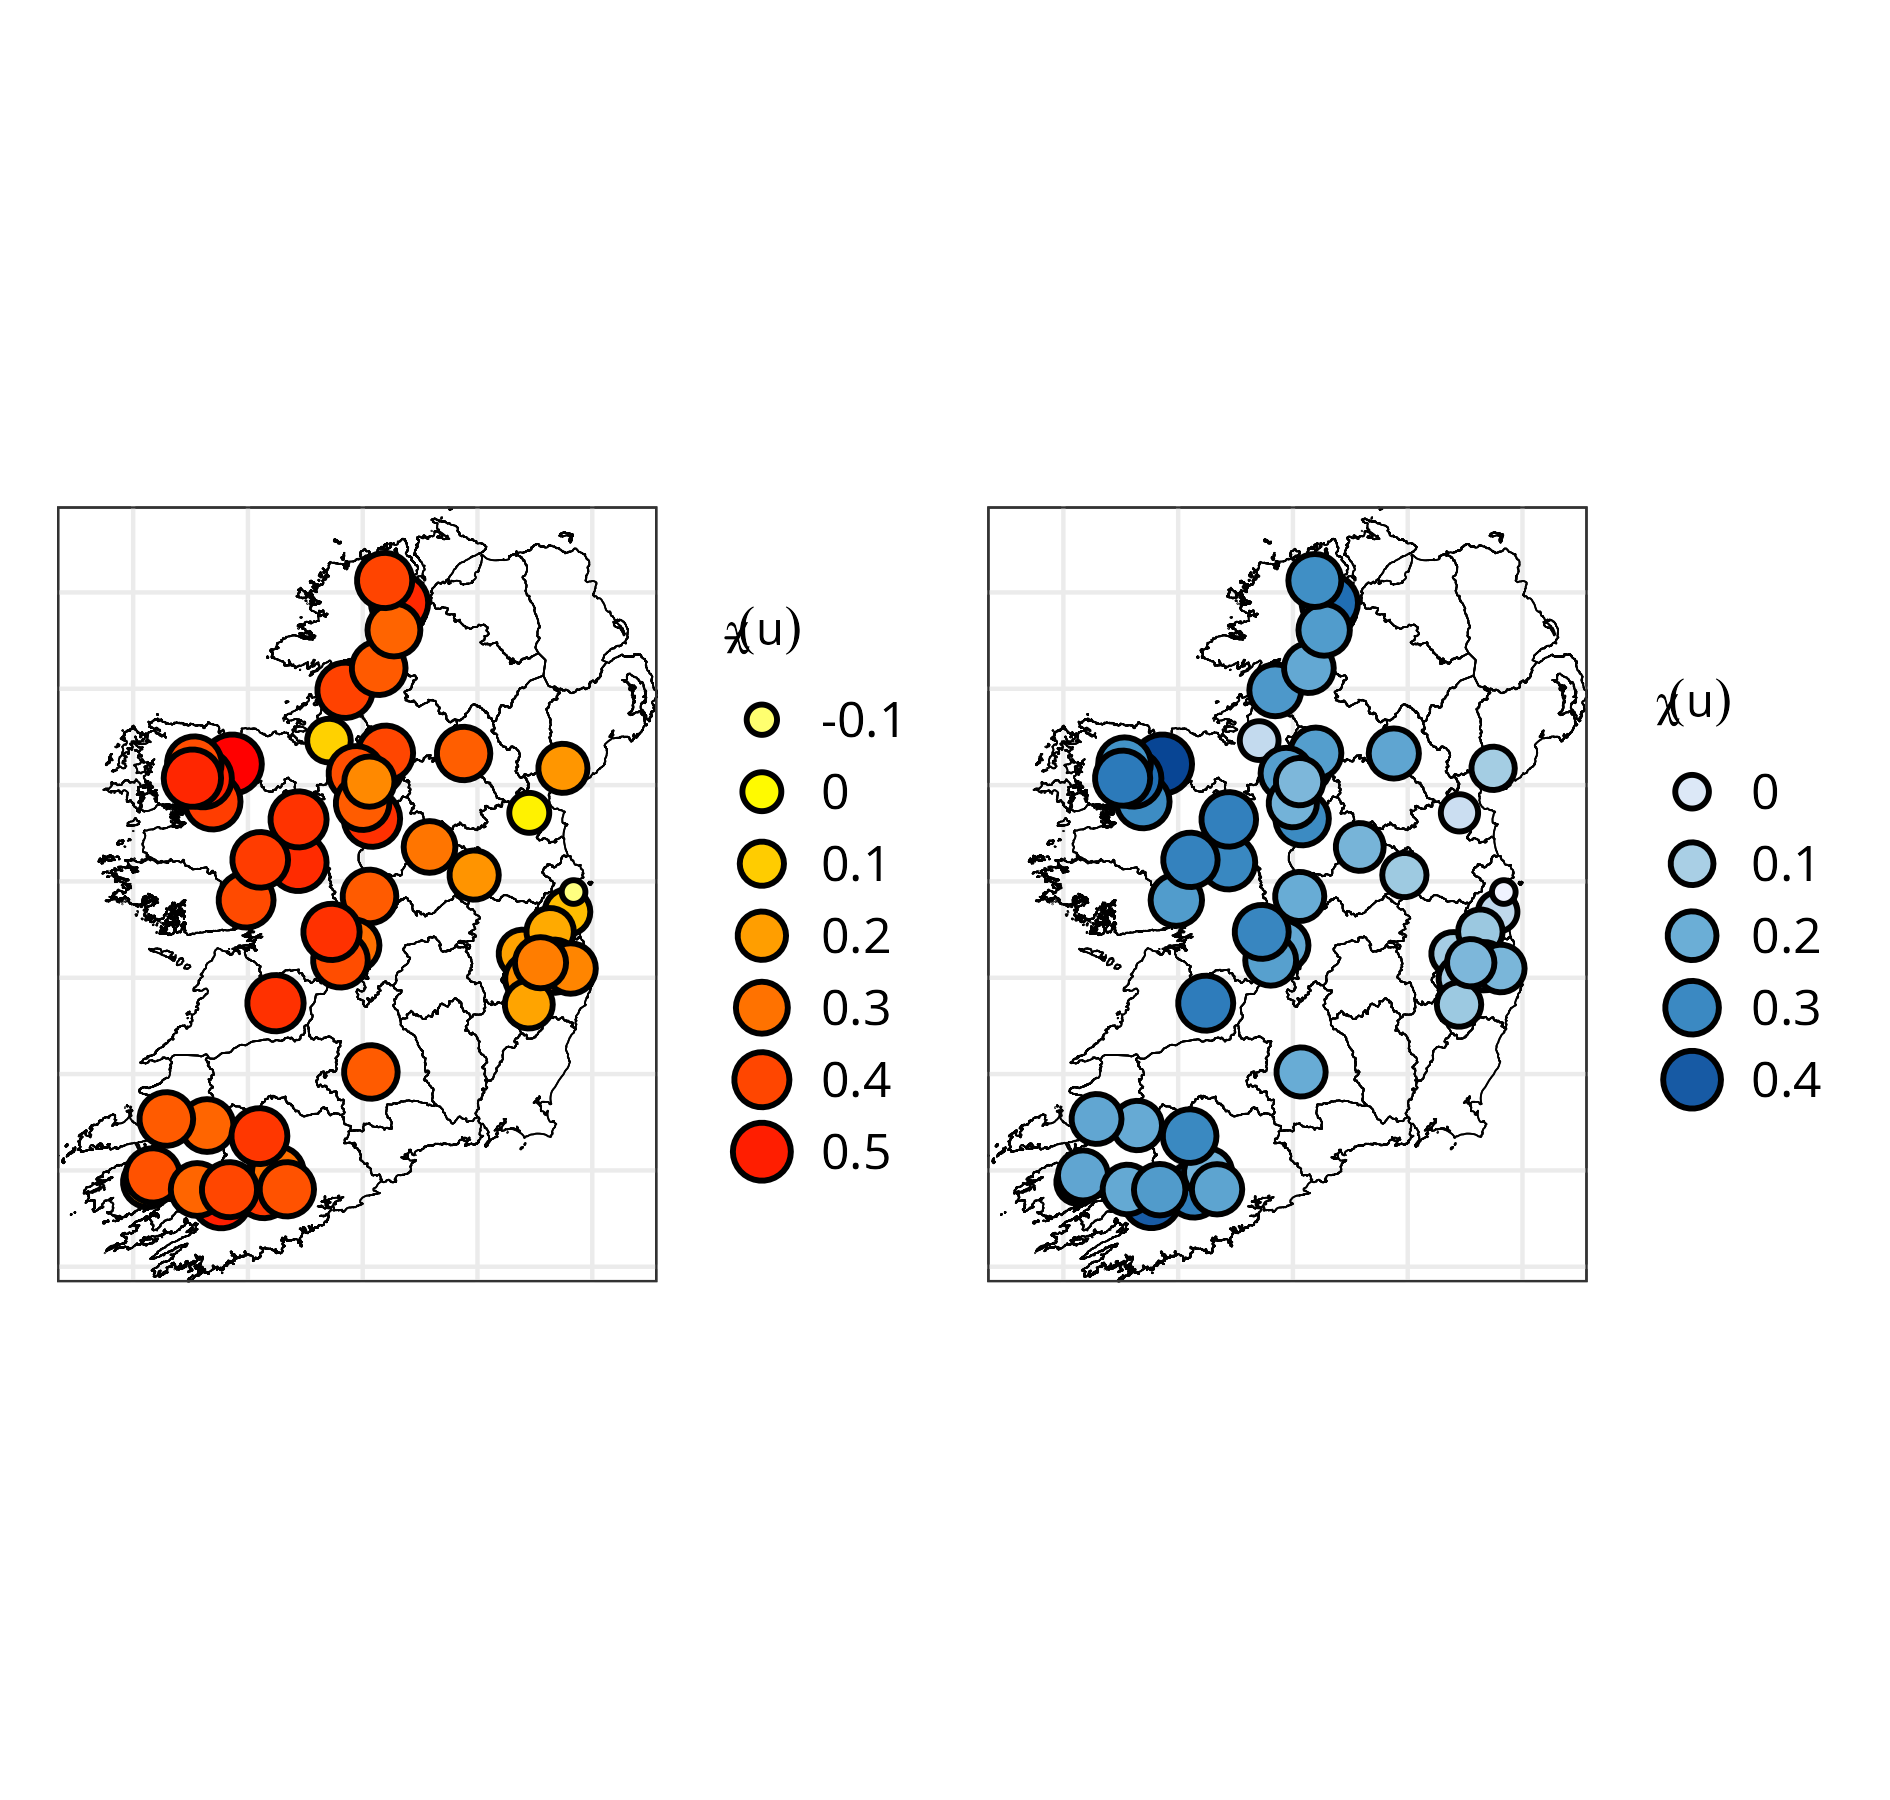
\includegraphics[width = 0.9\linewidth]{plots/041_chi_plots.png}
    \caption{\emph{Test}}
    \label{fig:04_chi}
\end{figure}

% Plot bootstrapping results for one location
\begin{figure}[H]
    \centering
    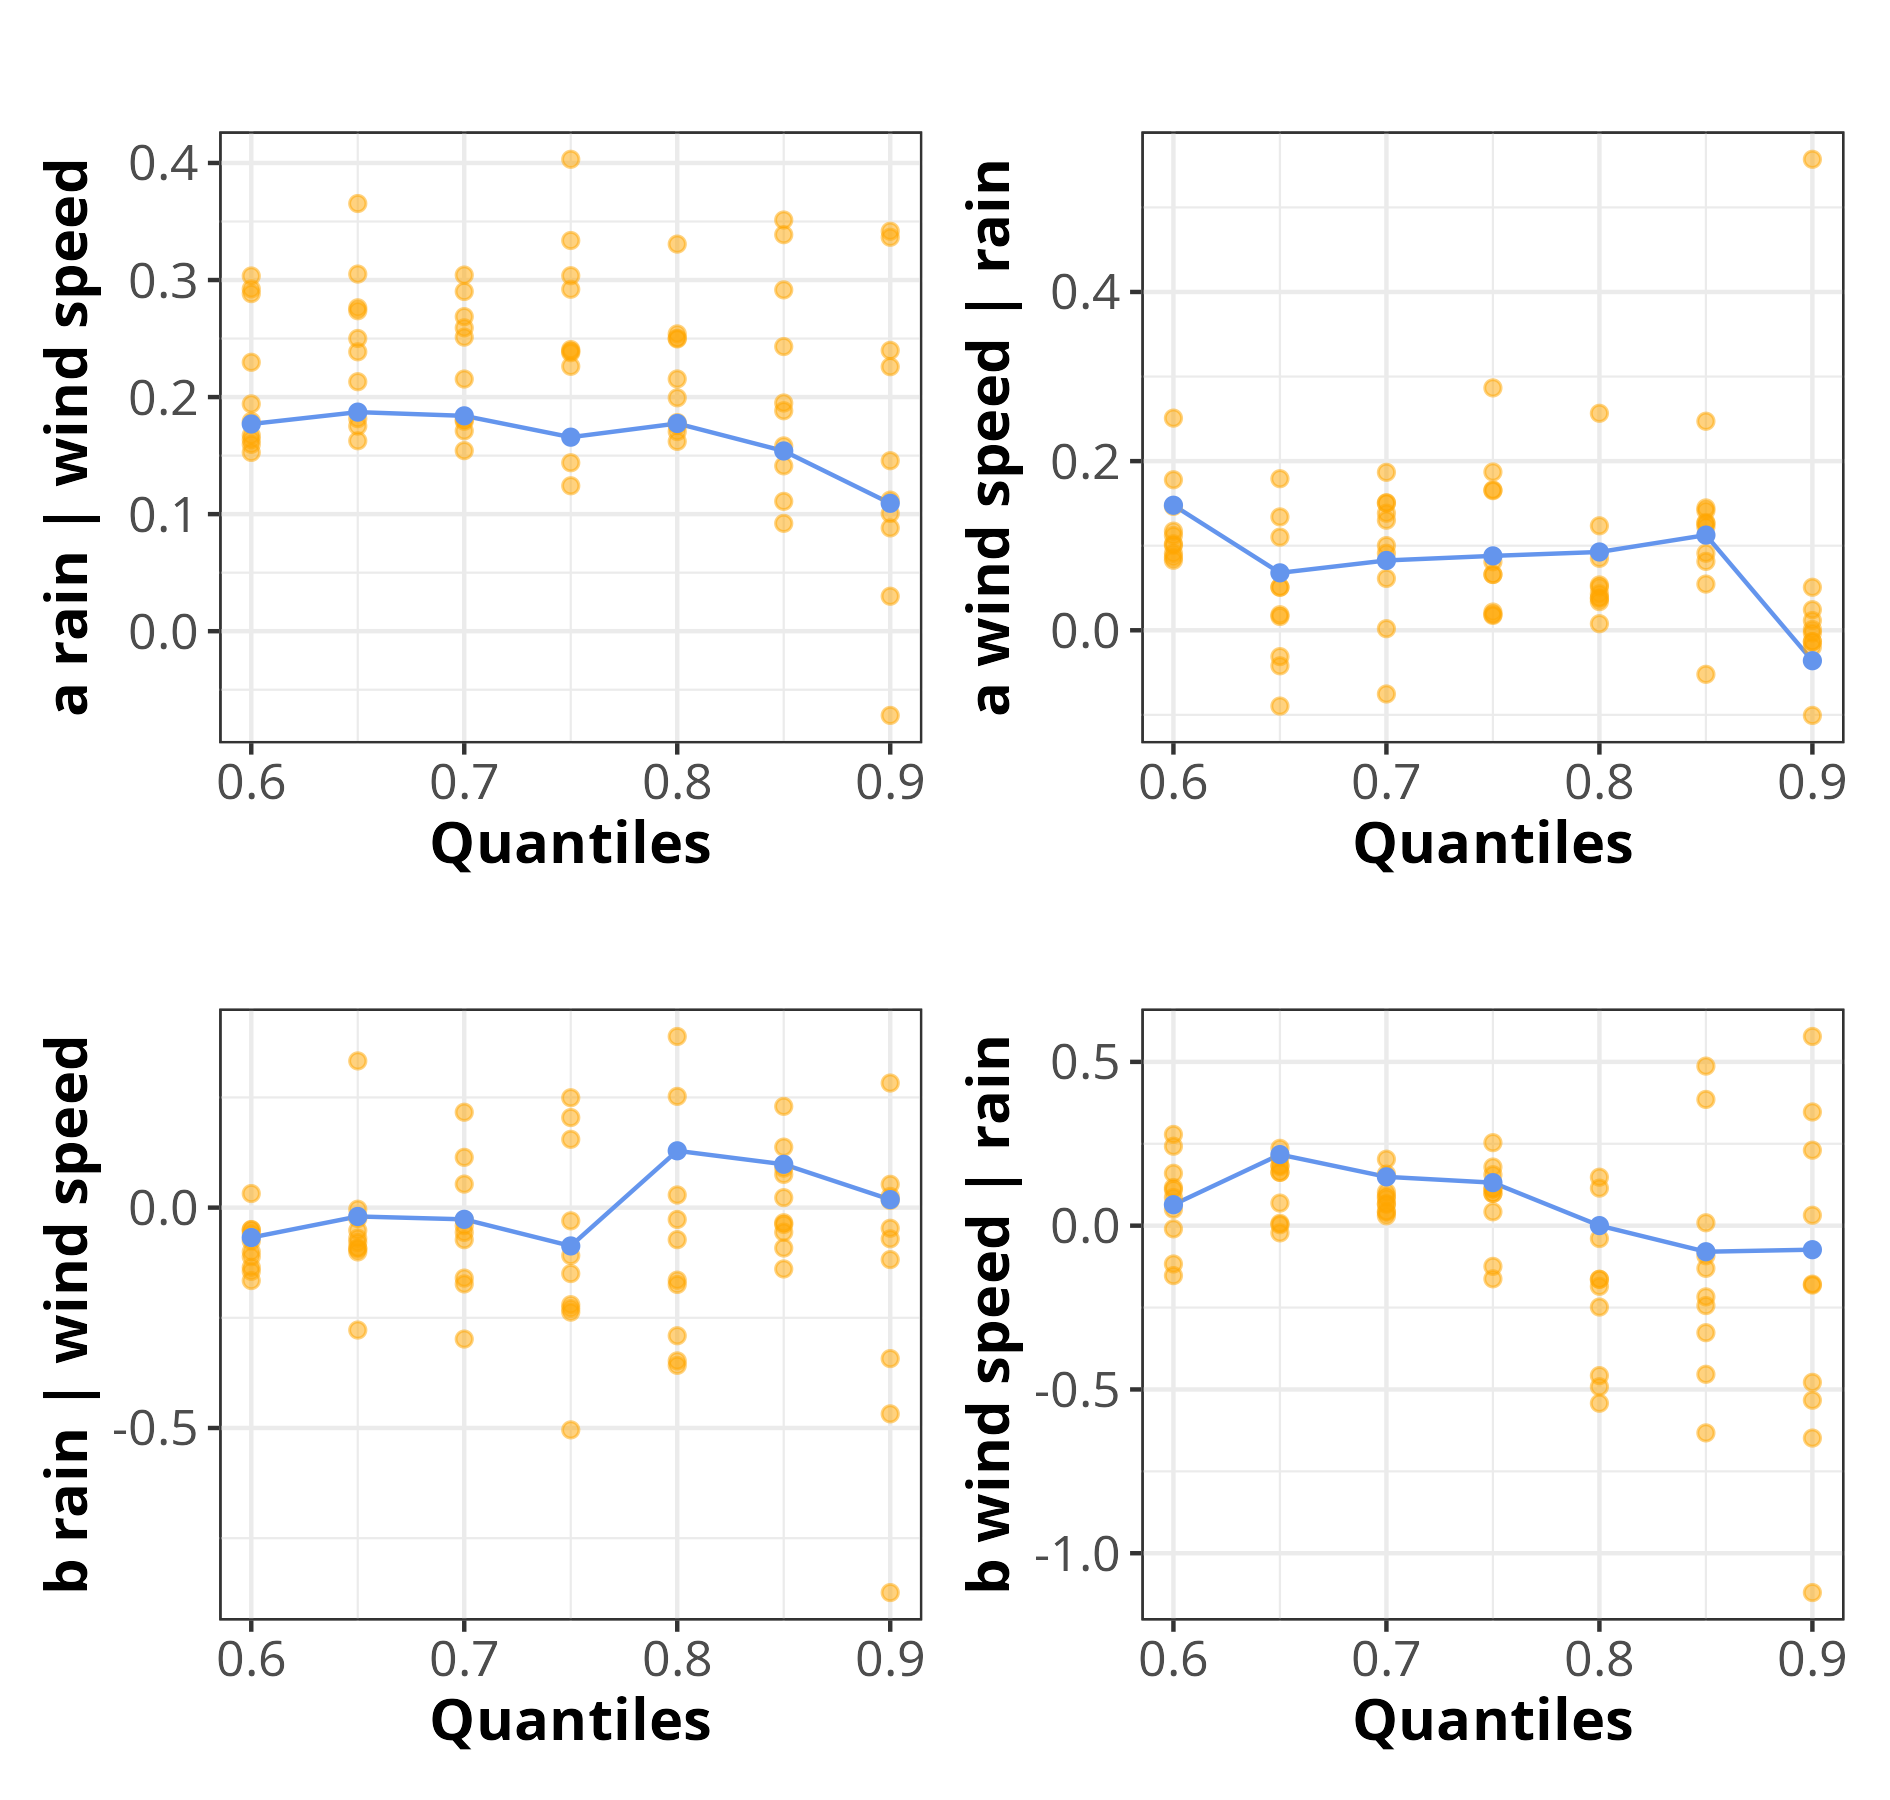
\includegraphics[width = 0.9\linewidth]{plots/042_bootstrap_thresh.png}
    \caption{\emph{Test}}
    \label{fig:04_bootstrap_thresh}
\end{figure}

% Profile likelihood showing uncertainty in alpha
% \begin{figure}[H]
%     \centering
%     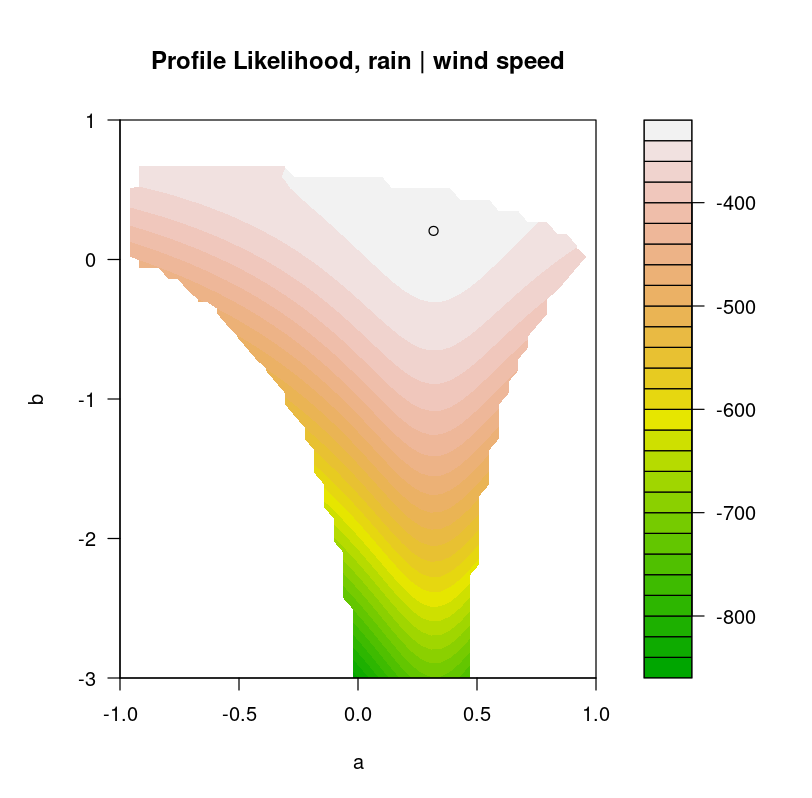
\includegraphics[width = 0.9\linewidth]{plots/043_prof_ll.png}
%     \caption{\emph{Test}}
%     \label{fig:04_prof_ll}
% \end{figure}
% 
% 
% % Bootstrap density for alpha, ultimate decision to fix beta
% \todo{Say for how many locations does alpha CI cross 0 (and also which bootstrapping fails for)}
% \begin{figure}[H]
%     \centering
%     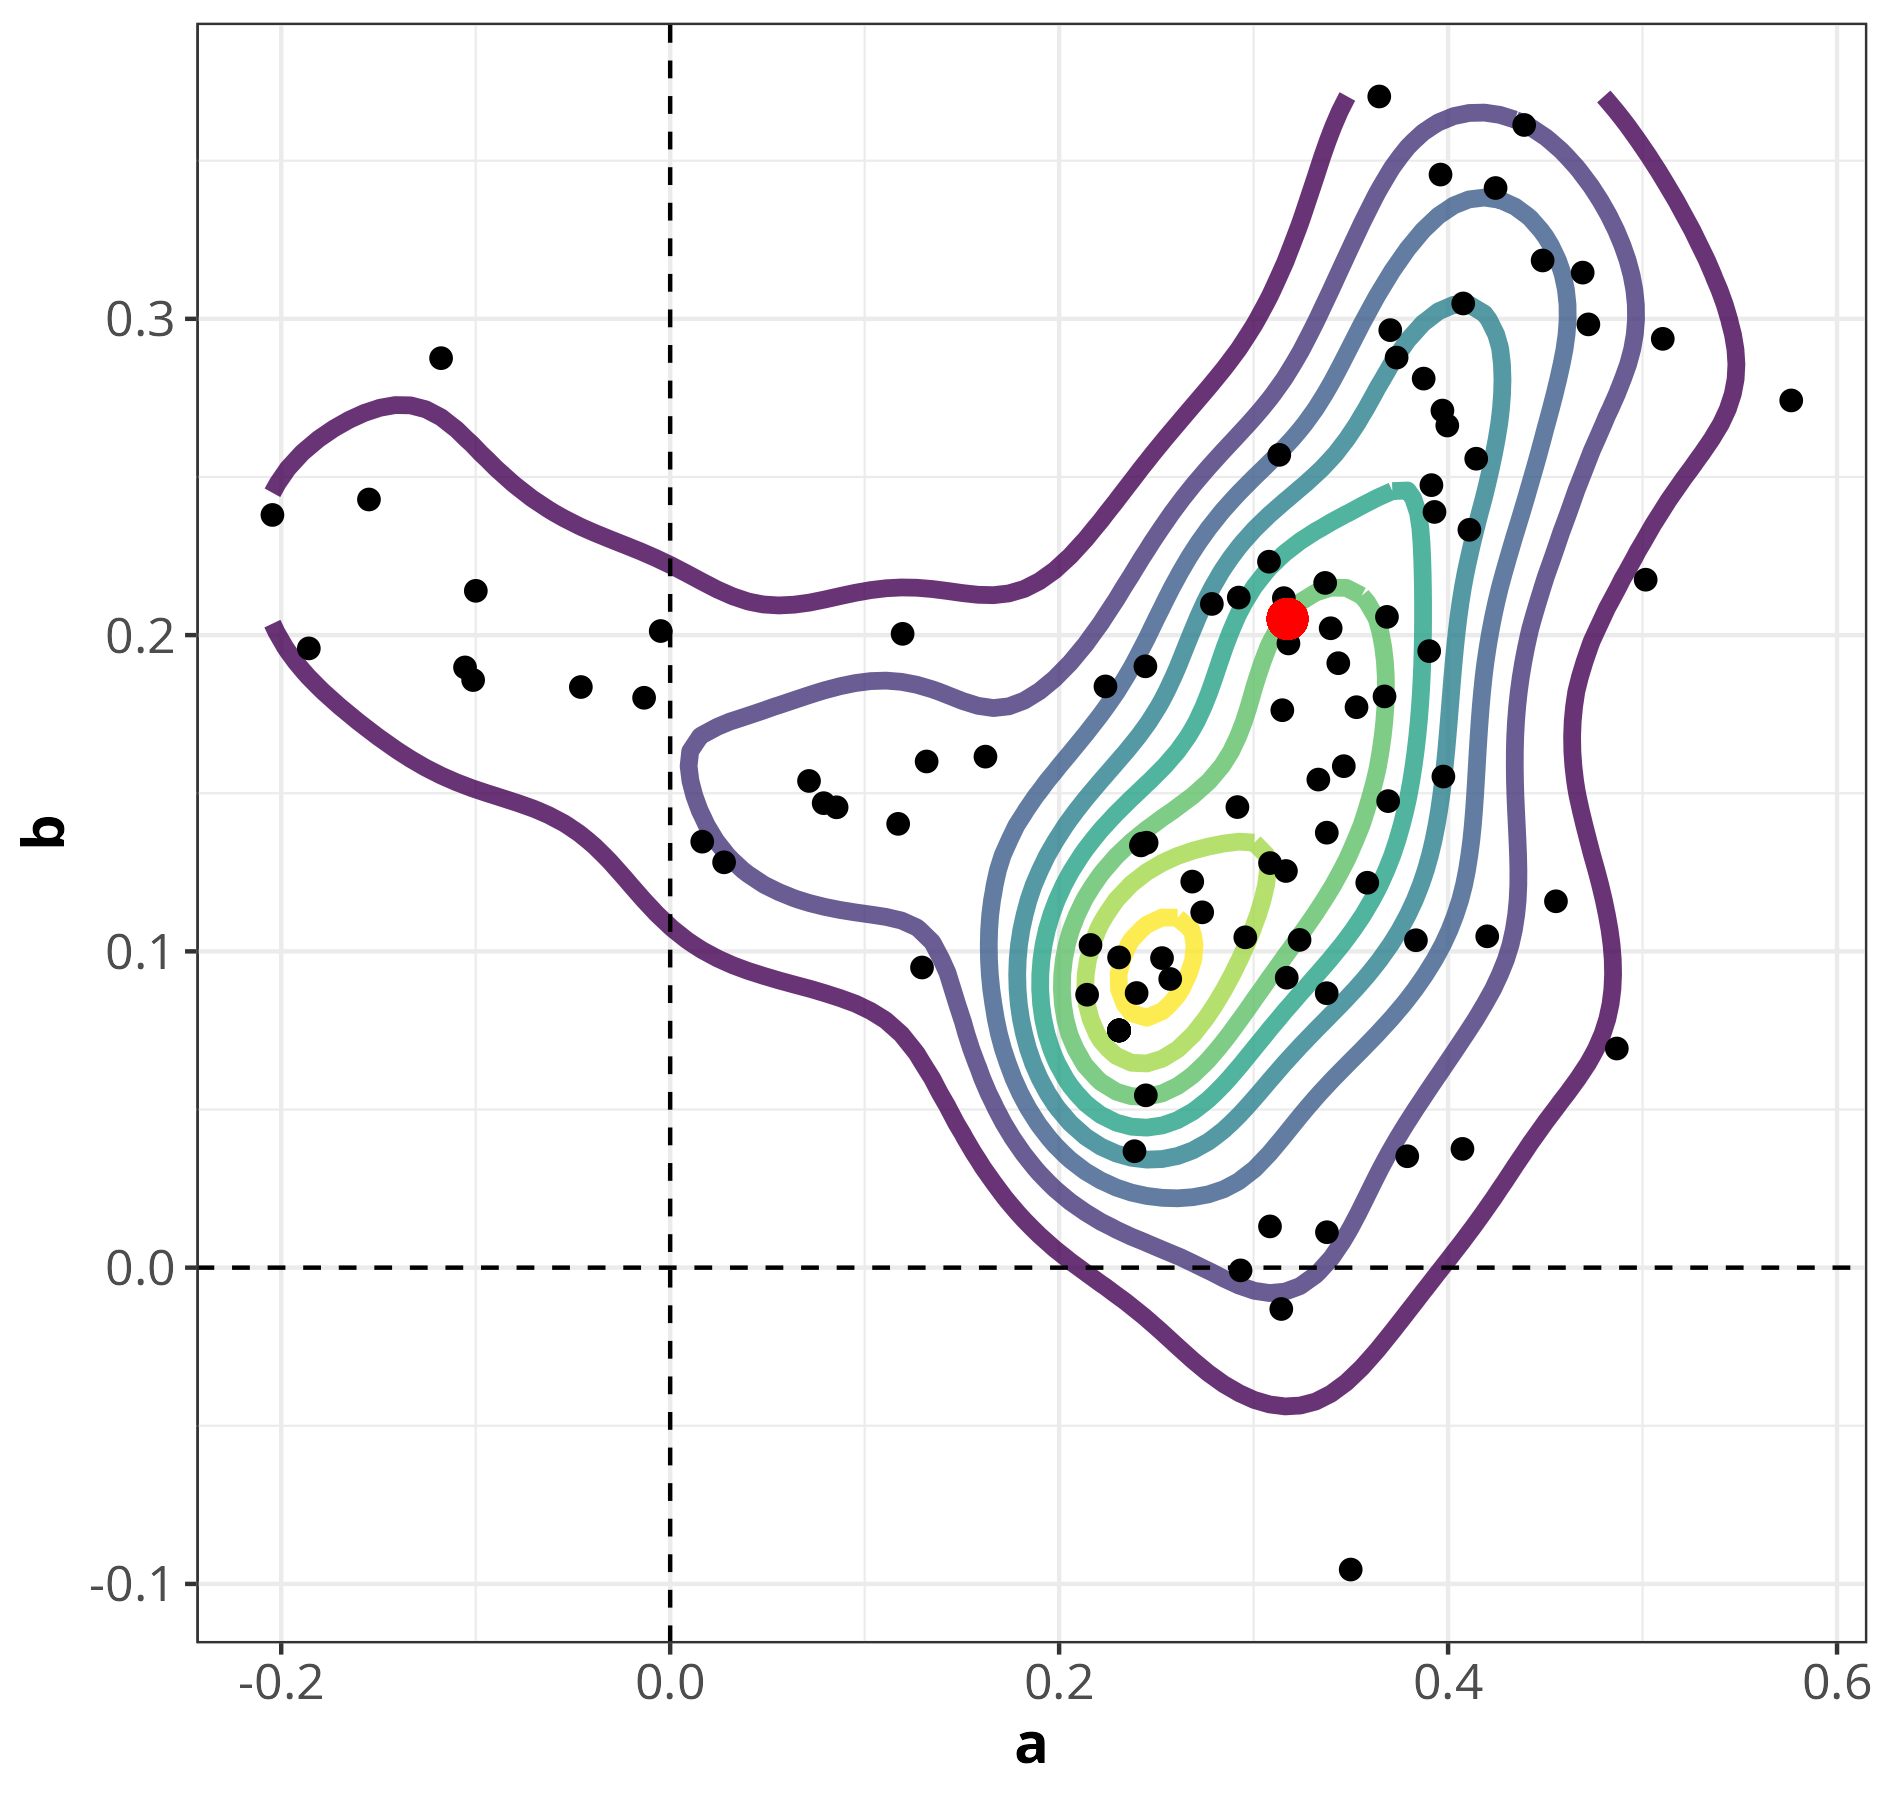
\includegraphics[width = 0.9\linewidth]{plots/044_bootstrap_density.png}
%     \caption{\emph{Test}}
%     \label{fig:04_density_alpha}
% \end{figure}

\begin{figure}[H]
    \centering
    \begin{minipage}{0.55\textwidth}
        \centering
        % 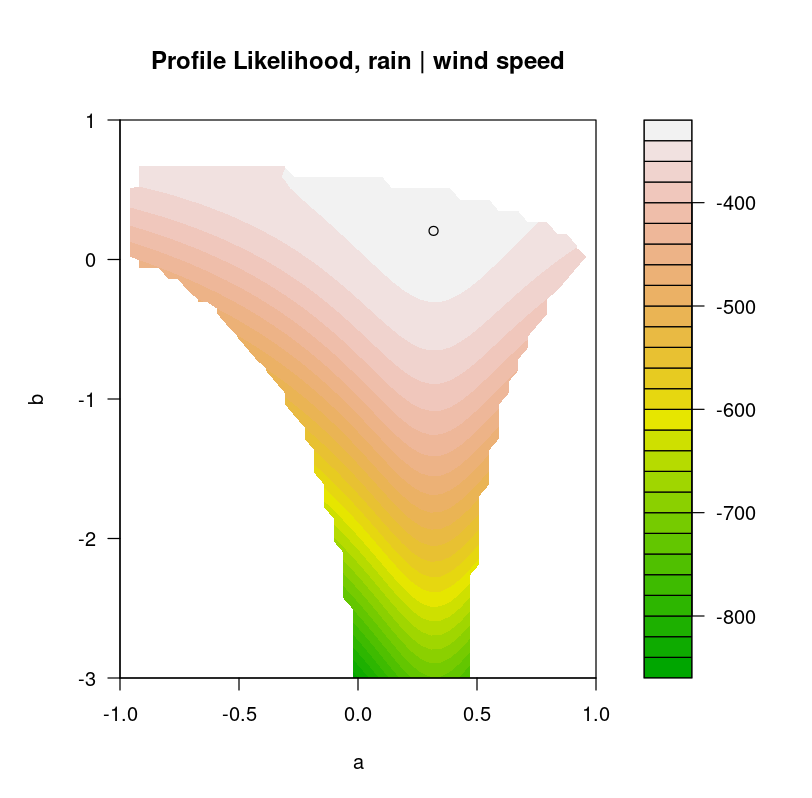
\includegraphics[width=\textwidth]{plots/043_prof_ll.png}
        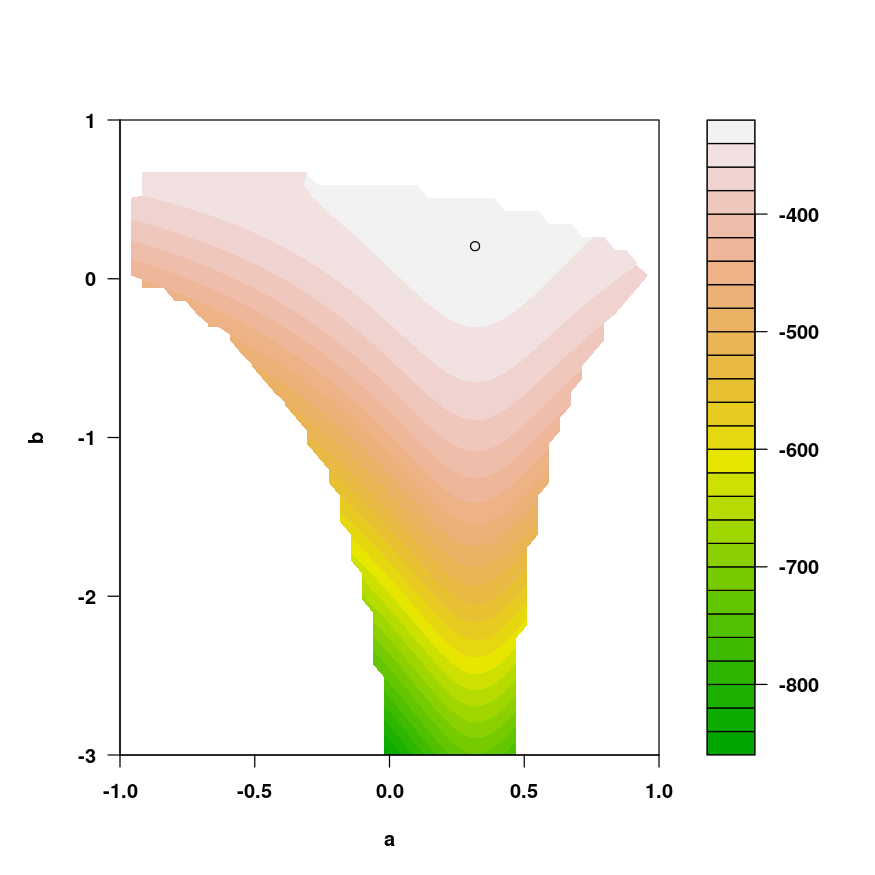
\includegraphics[width=\textwidth]{plots/Rplot01.png}
        % \caption{Plot 1}
        \label{fig:plot1}
    \end{minipage}
    \hfill
    \begin{minipage}{0.44\textwidth}
        \centering
        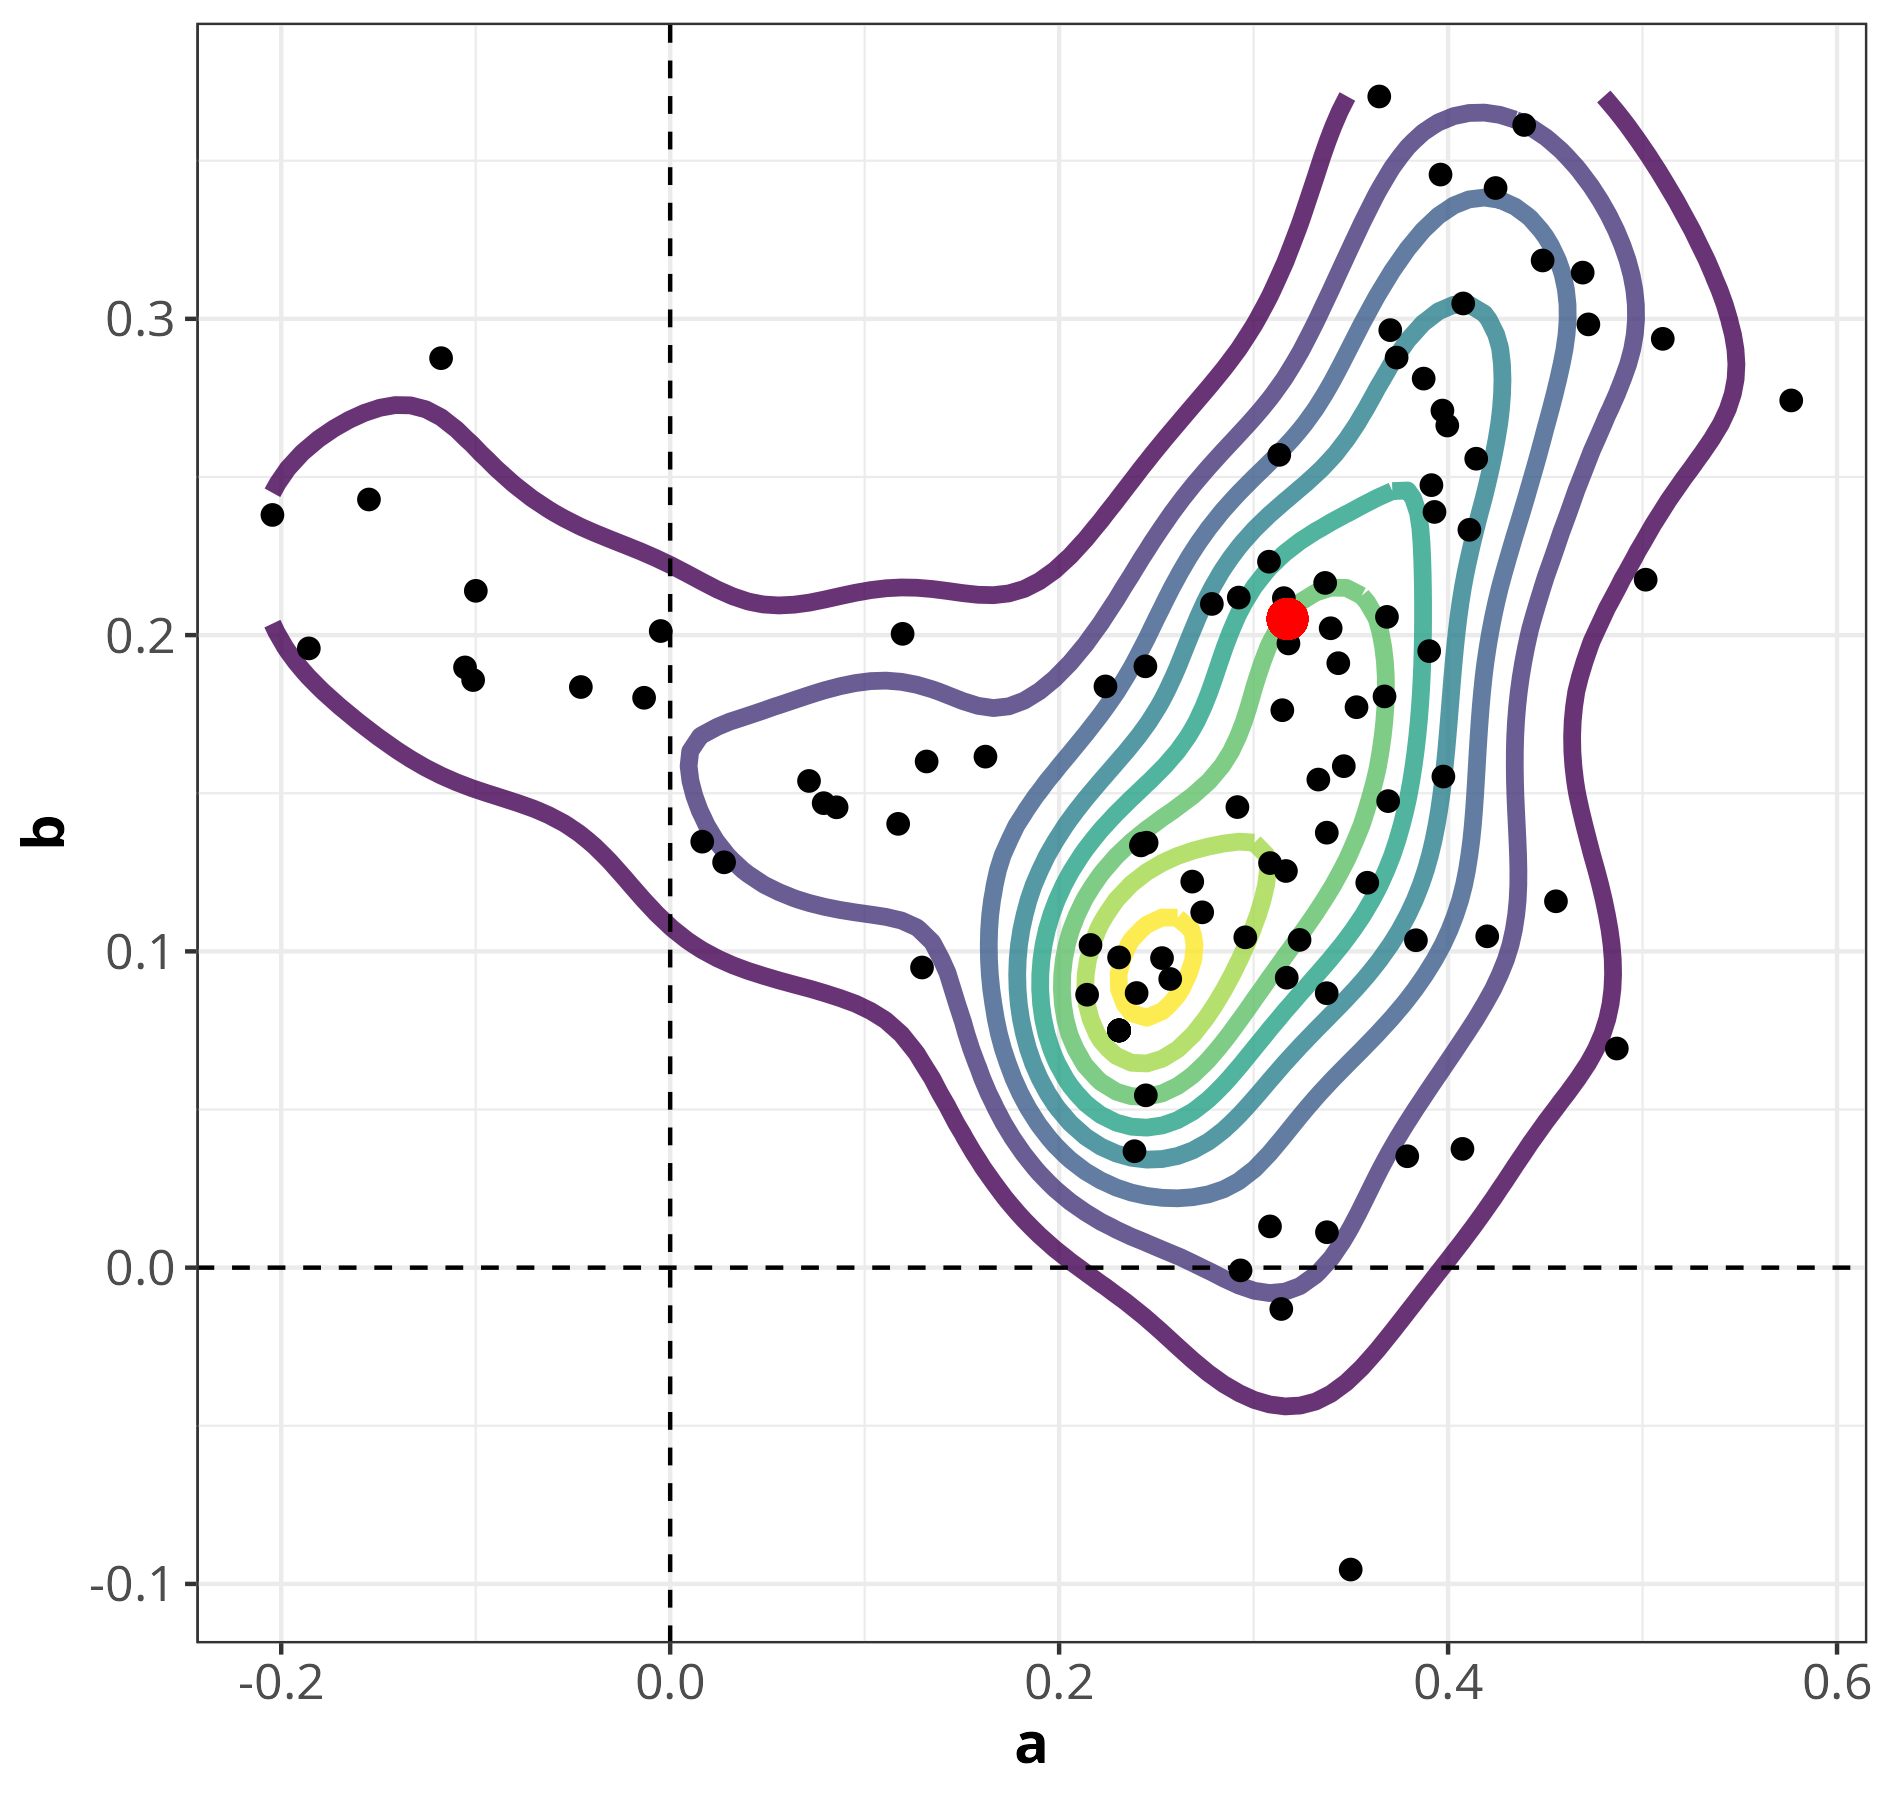
\includegraphics[width=\textwidth]{plots/044_bootstrap_density.png}
        % \caption{Plot 2}
        \label{fig:plot2}
    \end{minipage}
    \caption{Two plots side by side}
\end{figure}

% Map of alpha values for rain and wind speed
\begin{figure}[H]
    \centering
    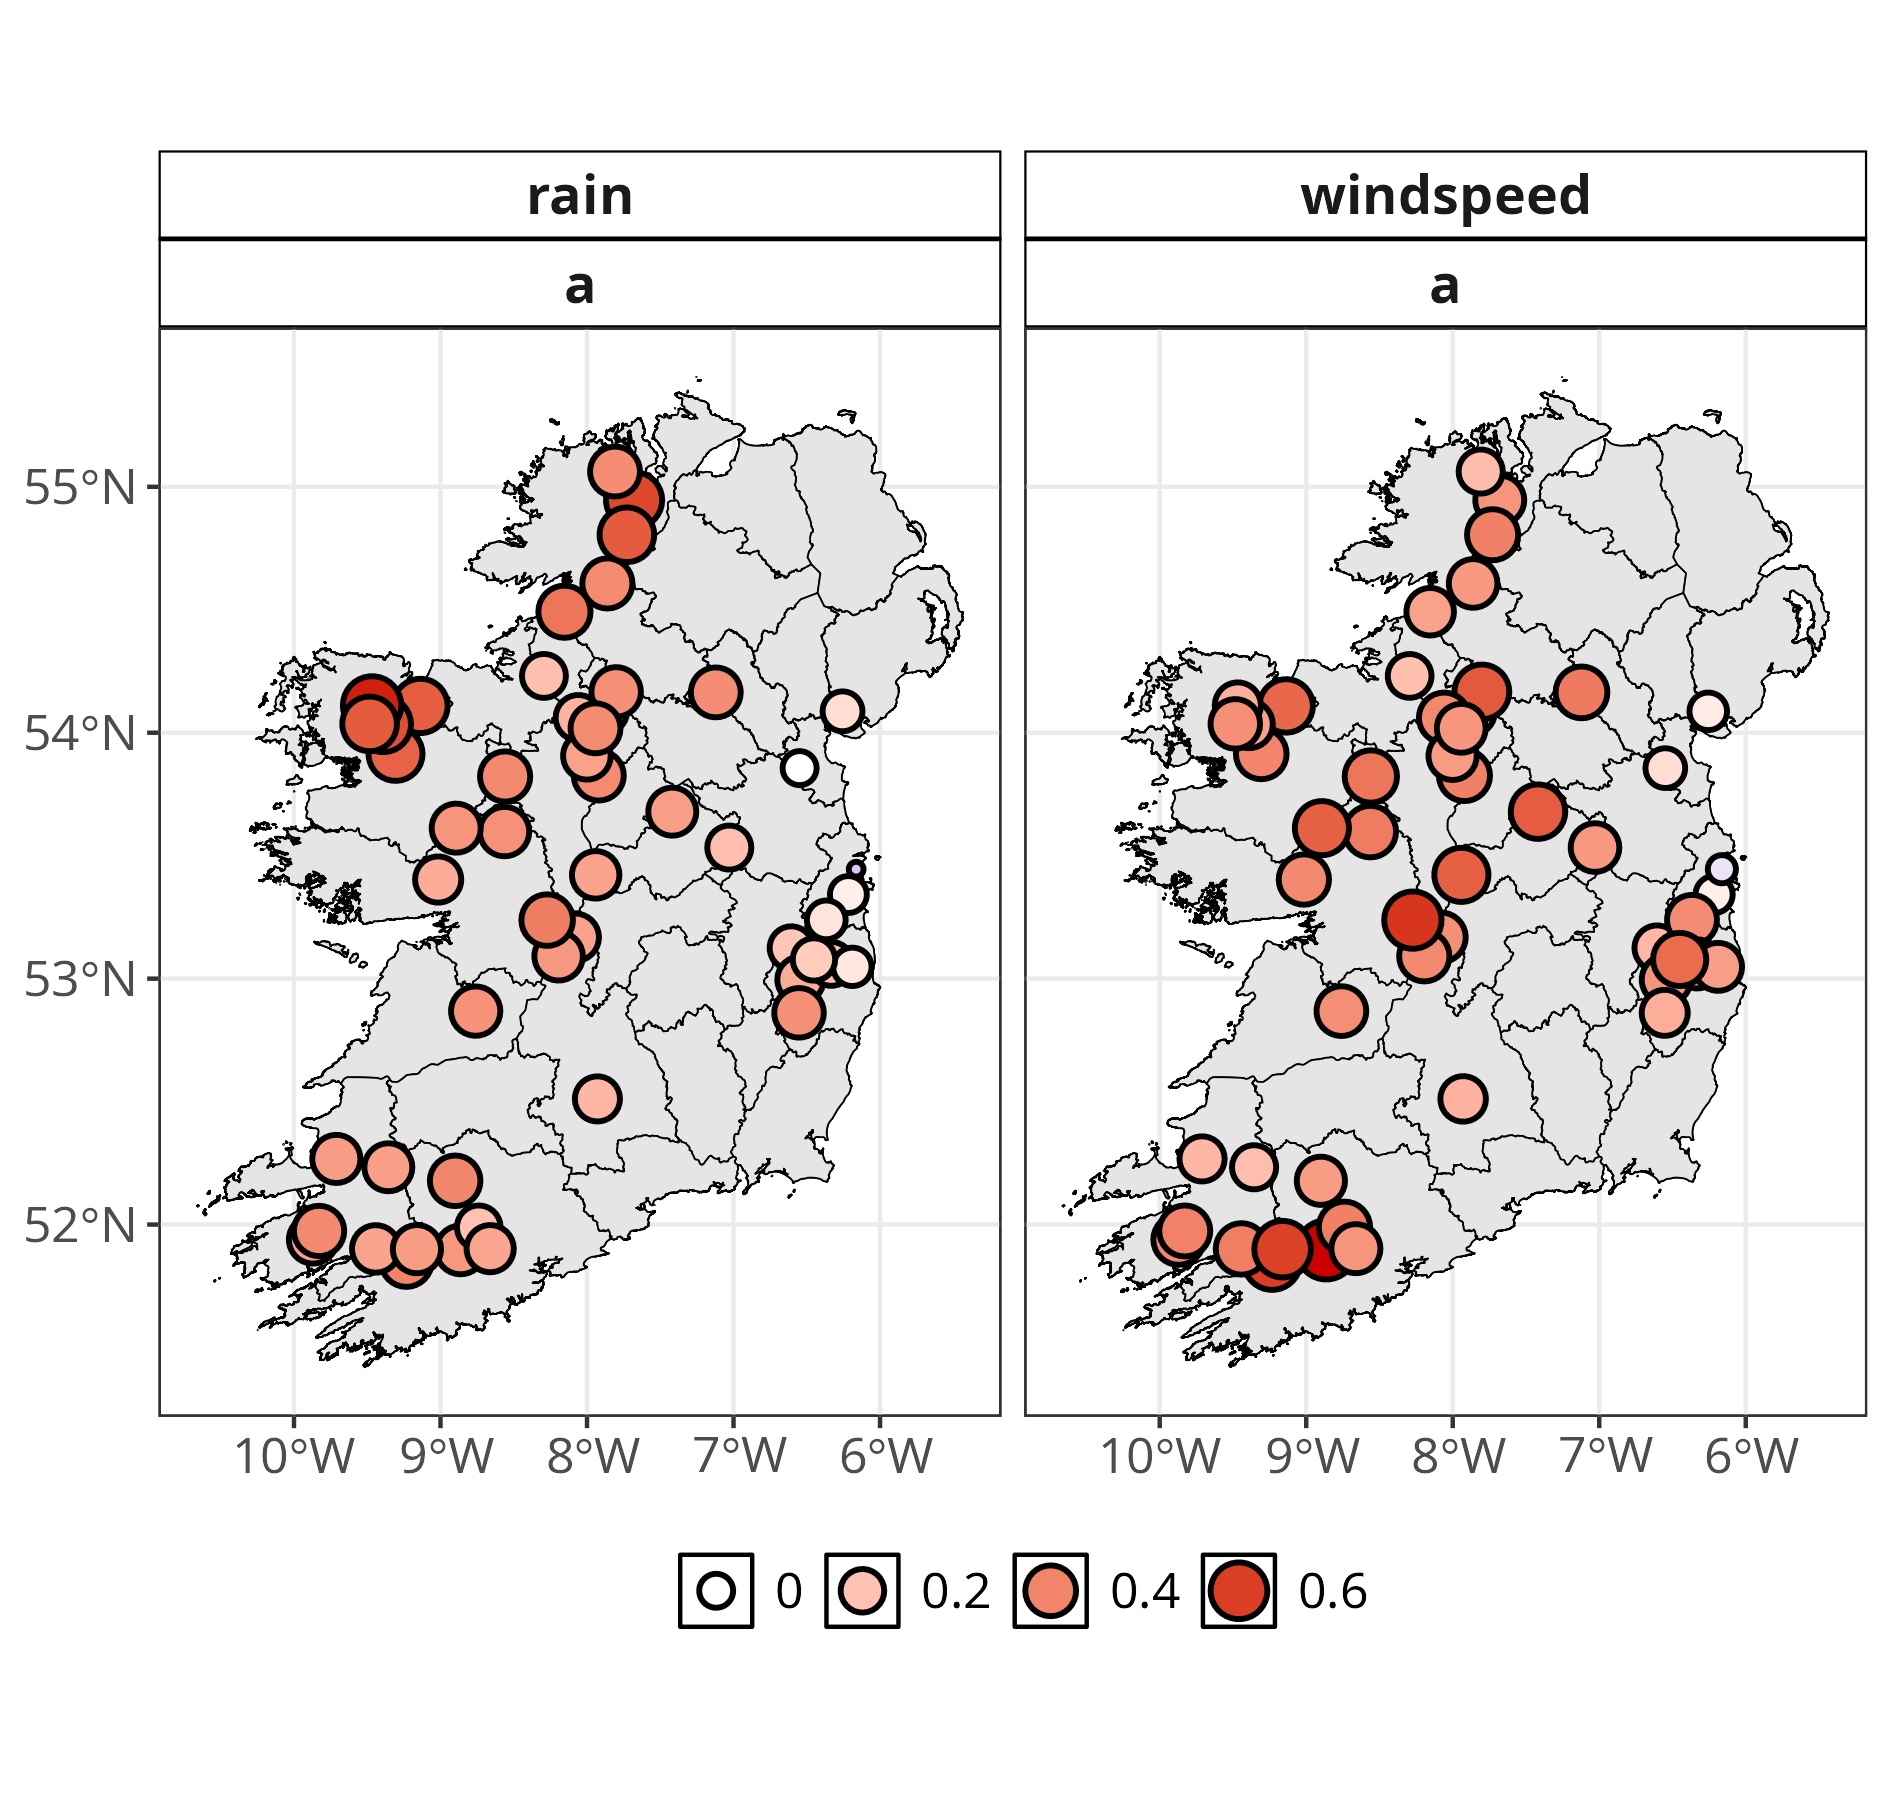
\includegraphics[width = 0.9\linewidth]{plots/045_alpha_map.png}
    \caption{\emph{Test}}
    \label{fig:04_alpha_map}
\end{figure}

% alpha values for rain vs wind speed
\begin{figure}[H]
    \centering
    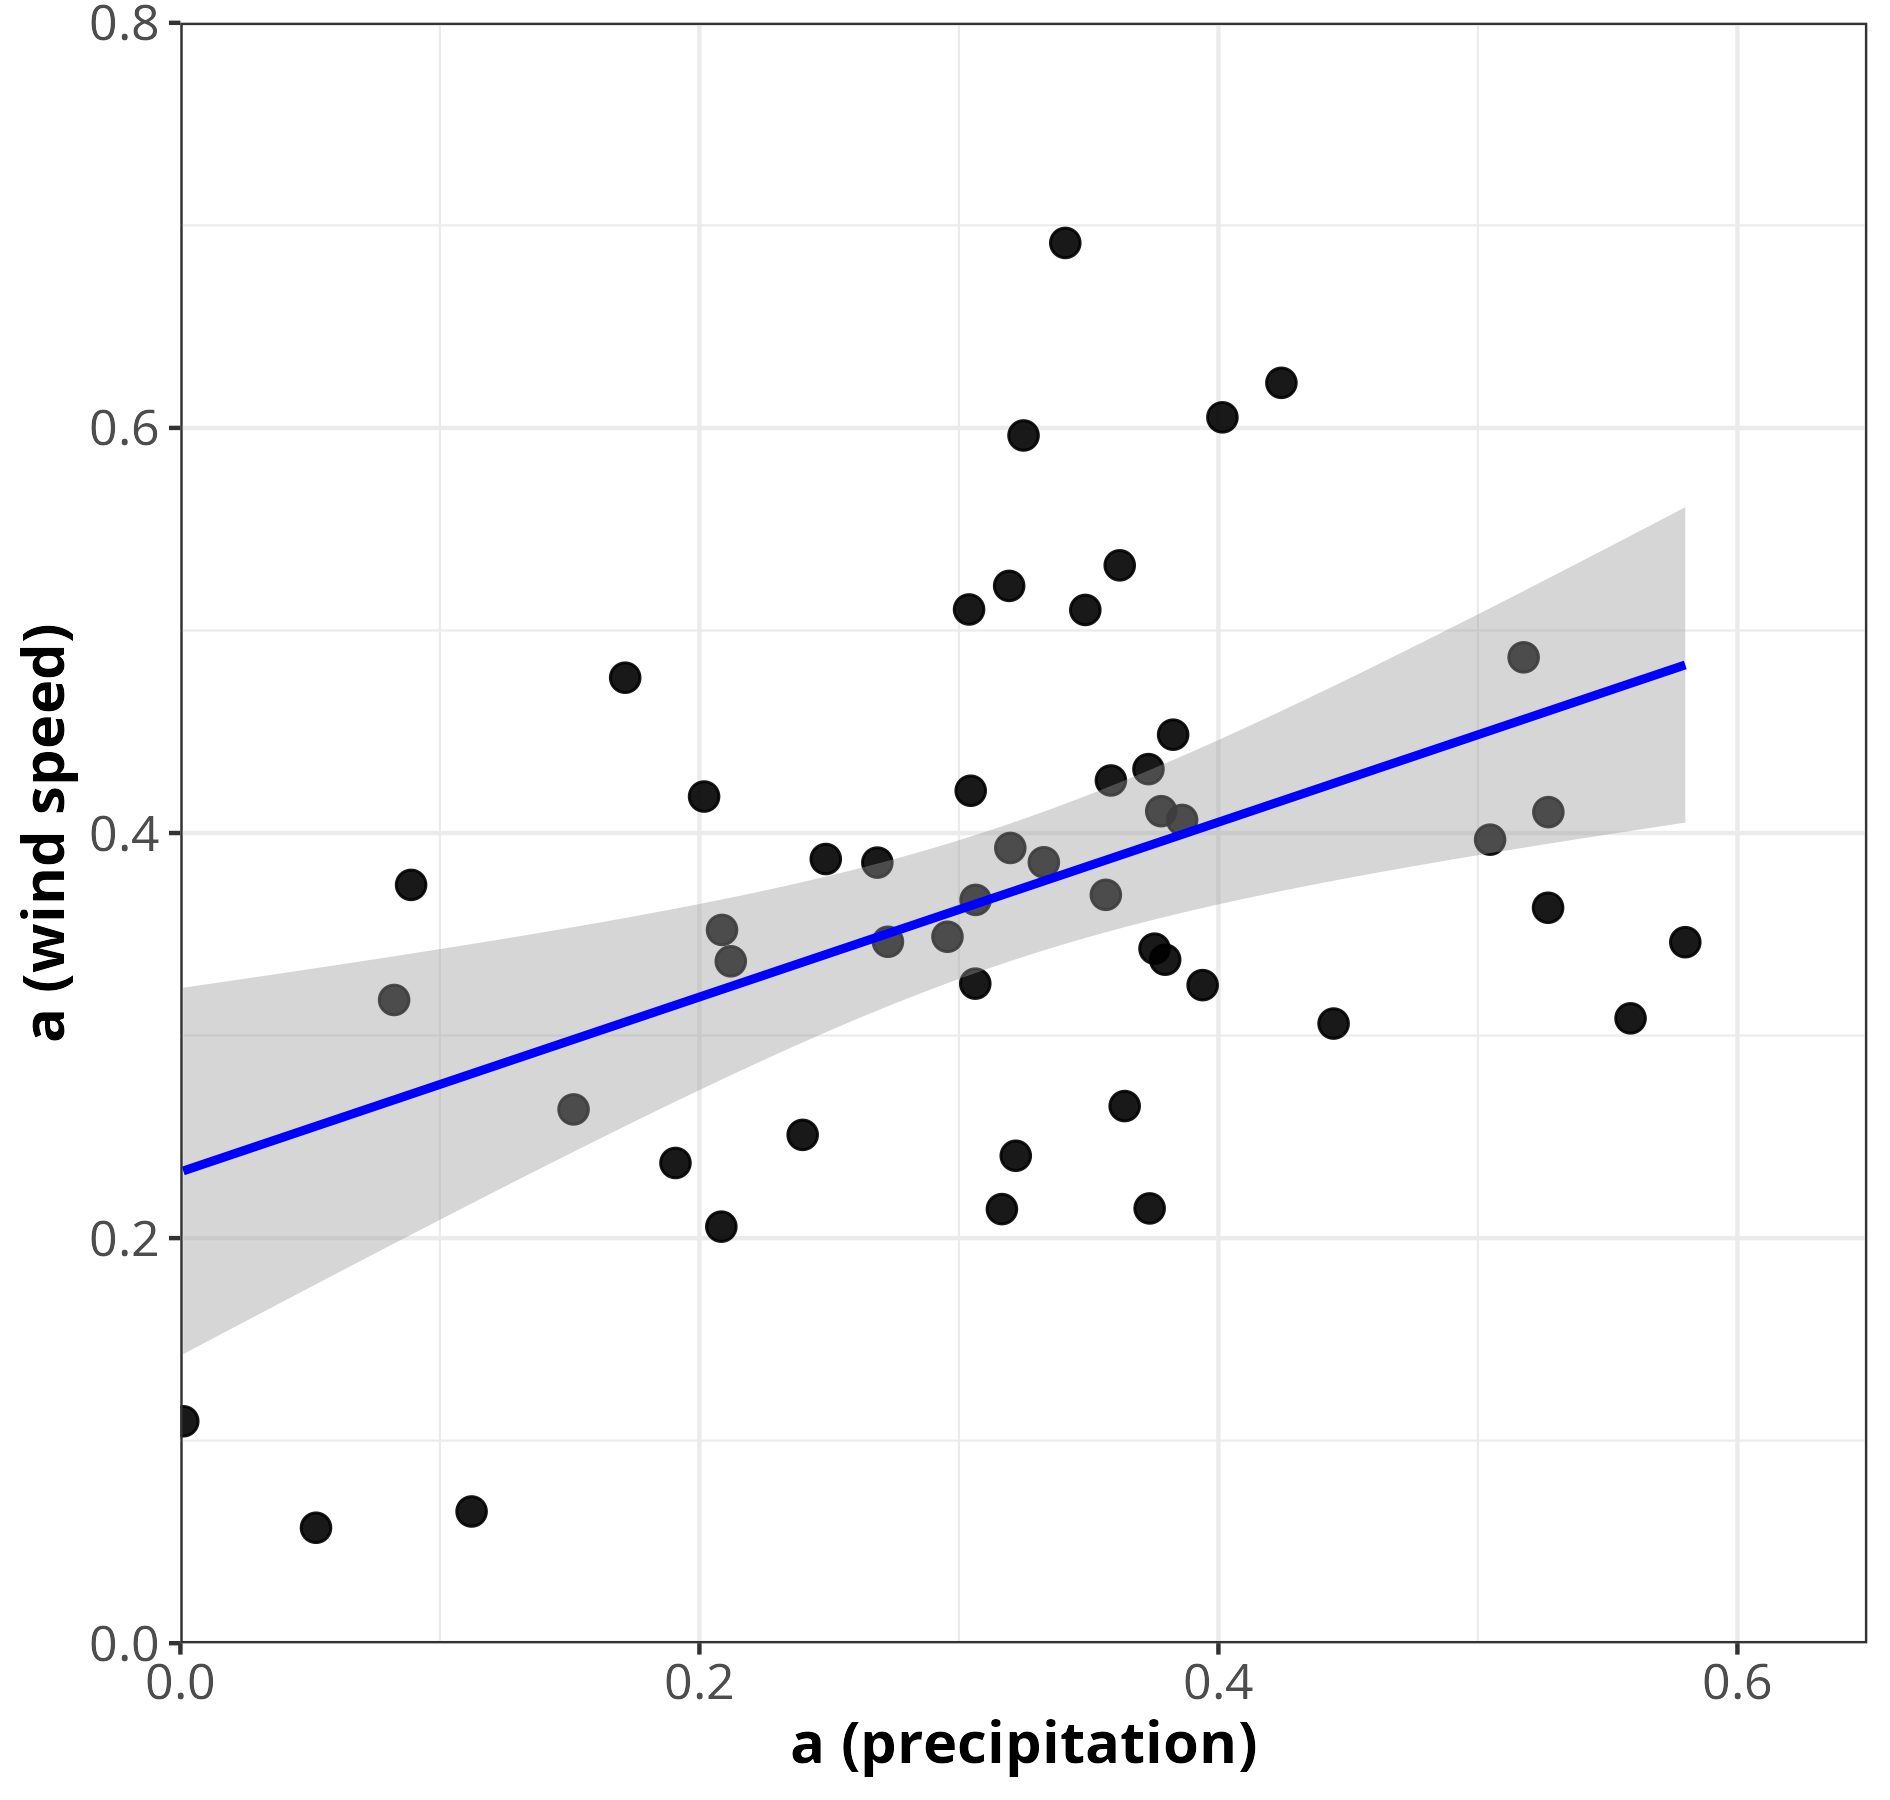
\includegraphics[width = 0.9\linewidth]{plots/046_alpha_rain_vs_ws.png}
    \caption{\emph{Test}}
    \label{fig:04_alpha_rain_vs_ws}
\end{figure}

% alpha values vs lon and lat
\begin{figure}[H]
    \centering
    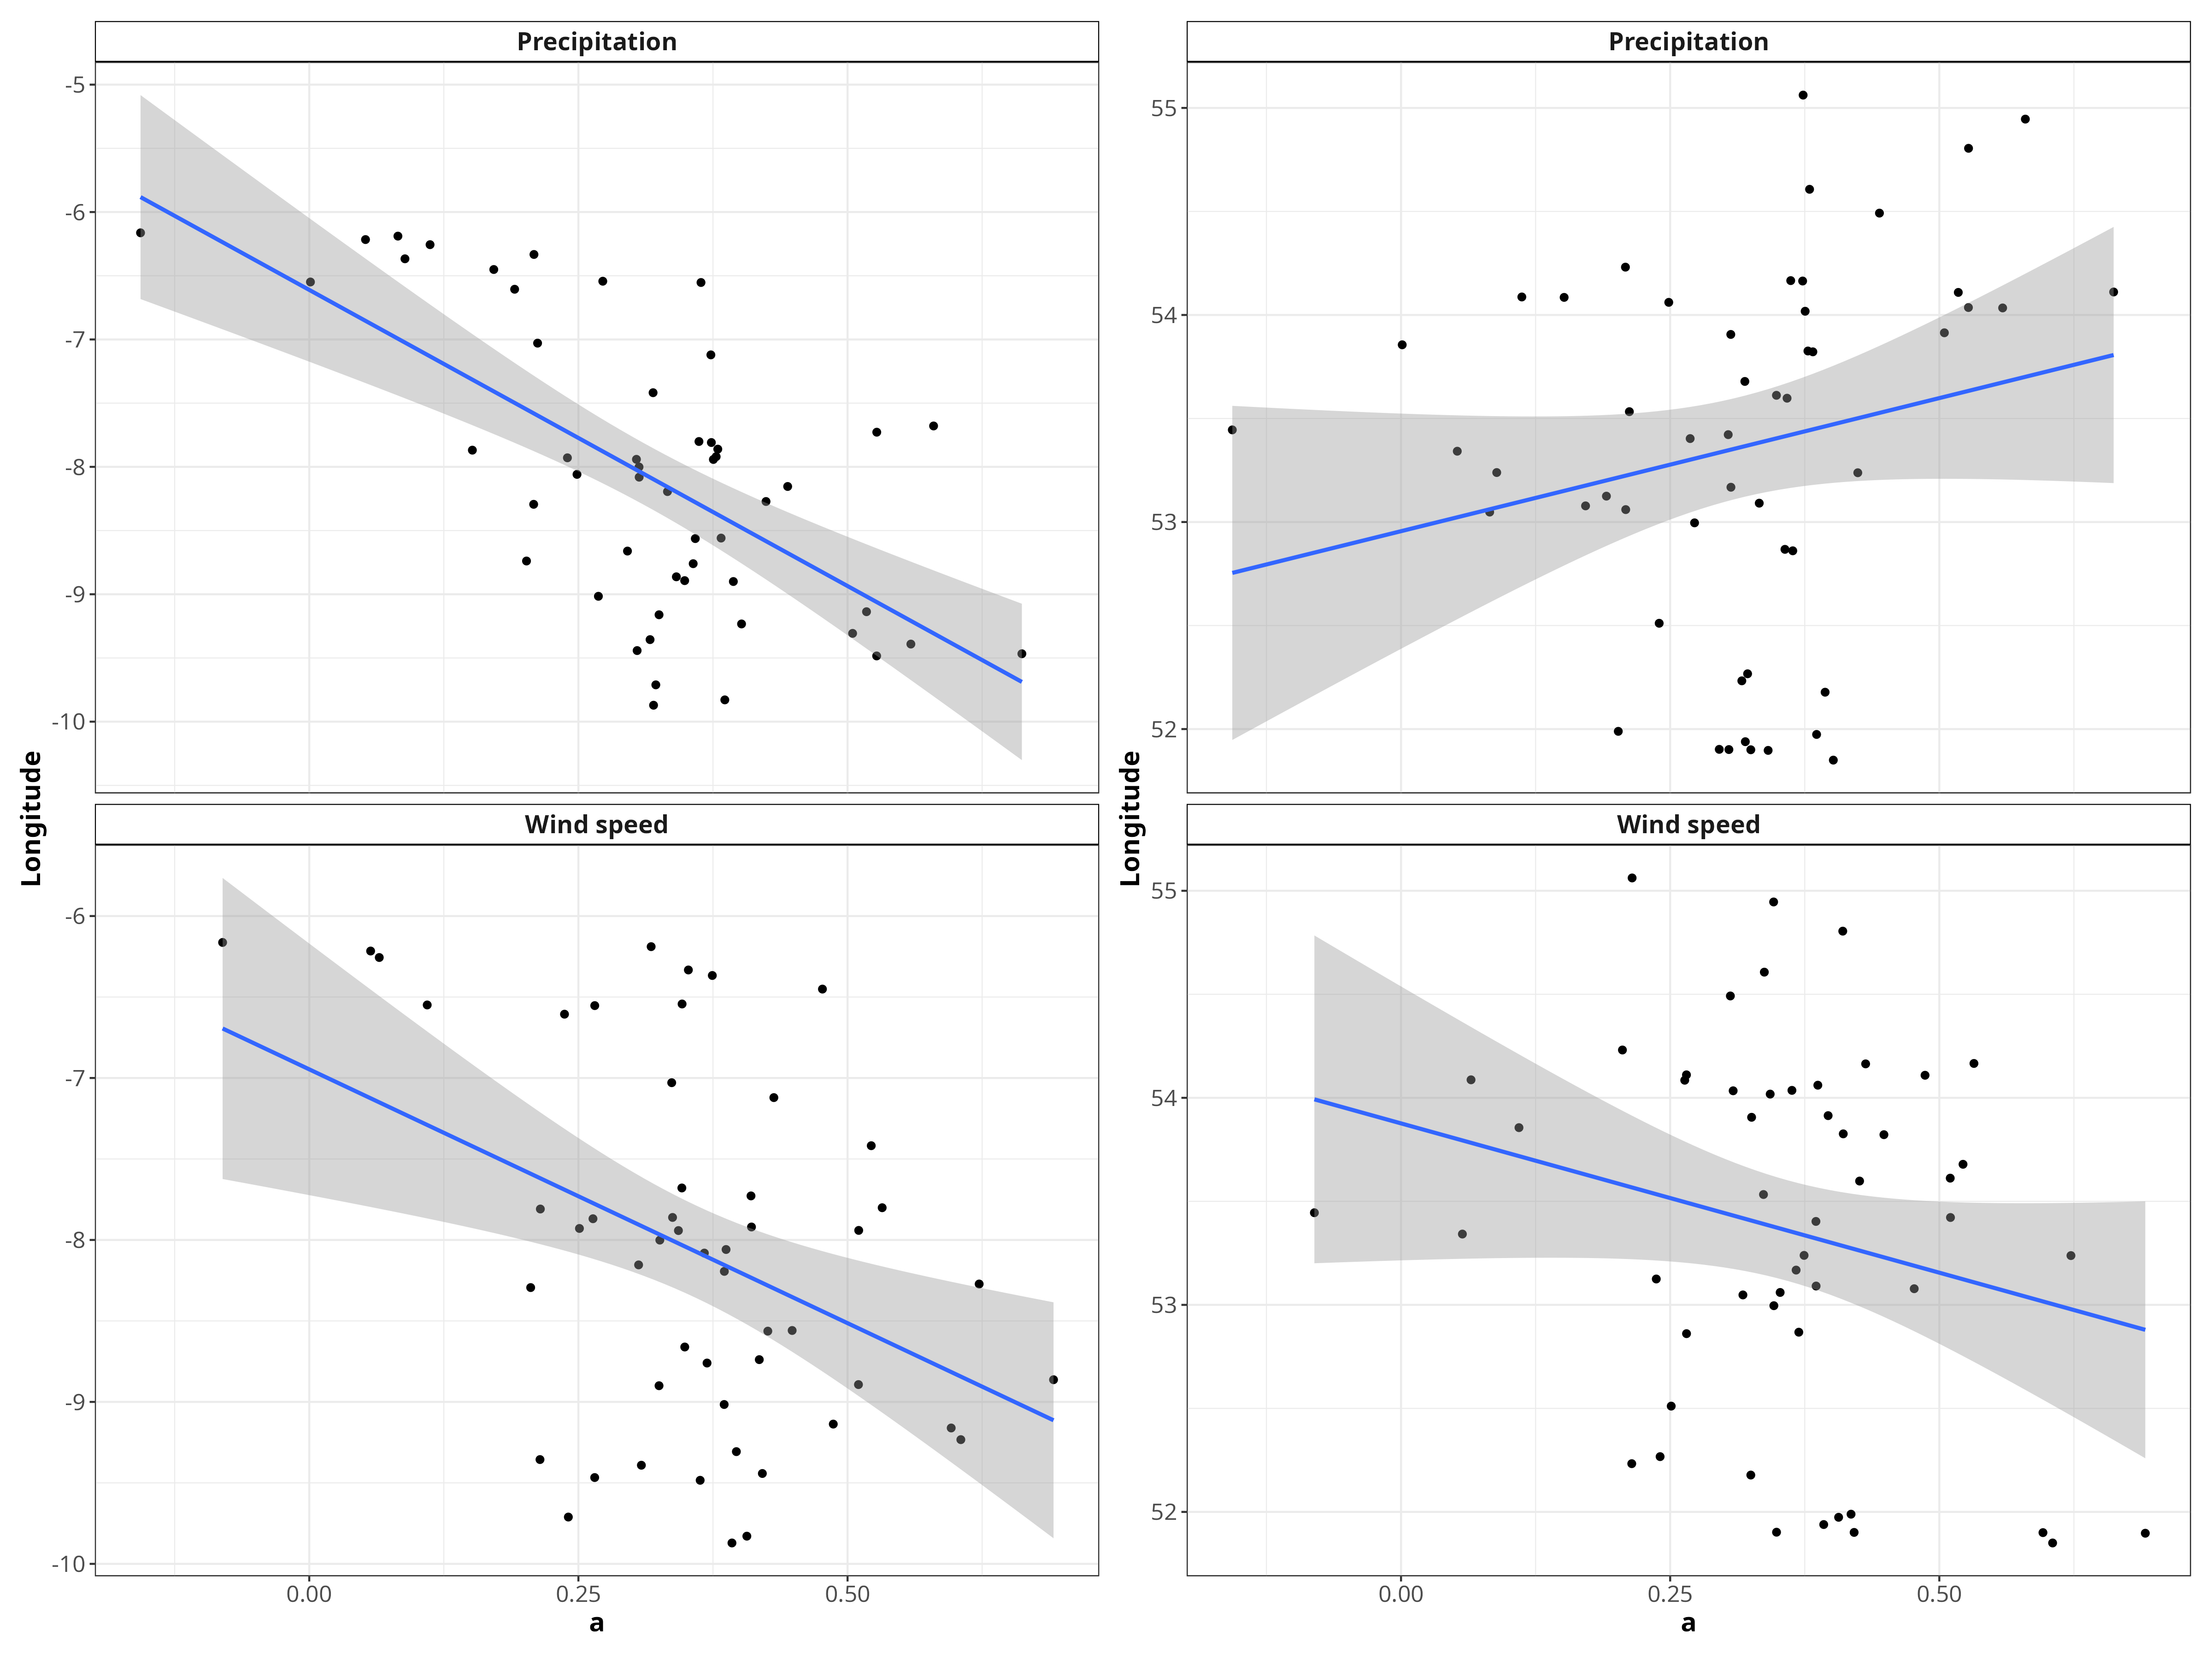
\includegraphics[width = 0.9\linewidth]{plots/047_alpha_vs_lon_lat.png}
    \caption{\emph{Test}}
    \label{fig:04_alpha_vs_lon_lat}
\end{figure}

% Individual diagnostic plots for some location
\begin{figure}[H]
    \centering
    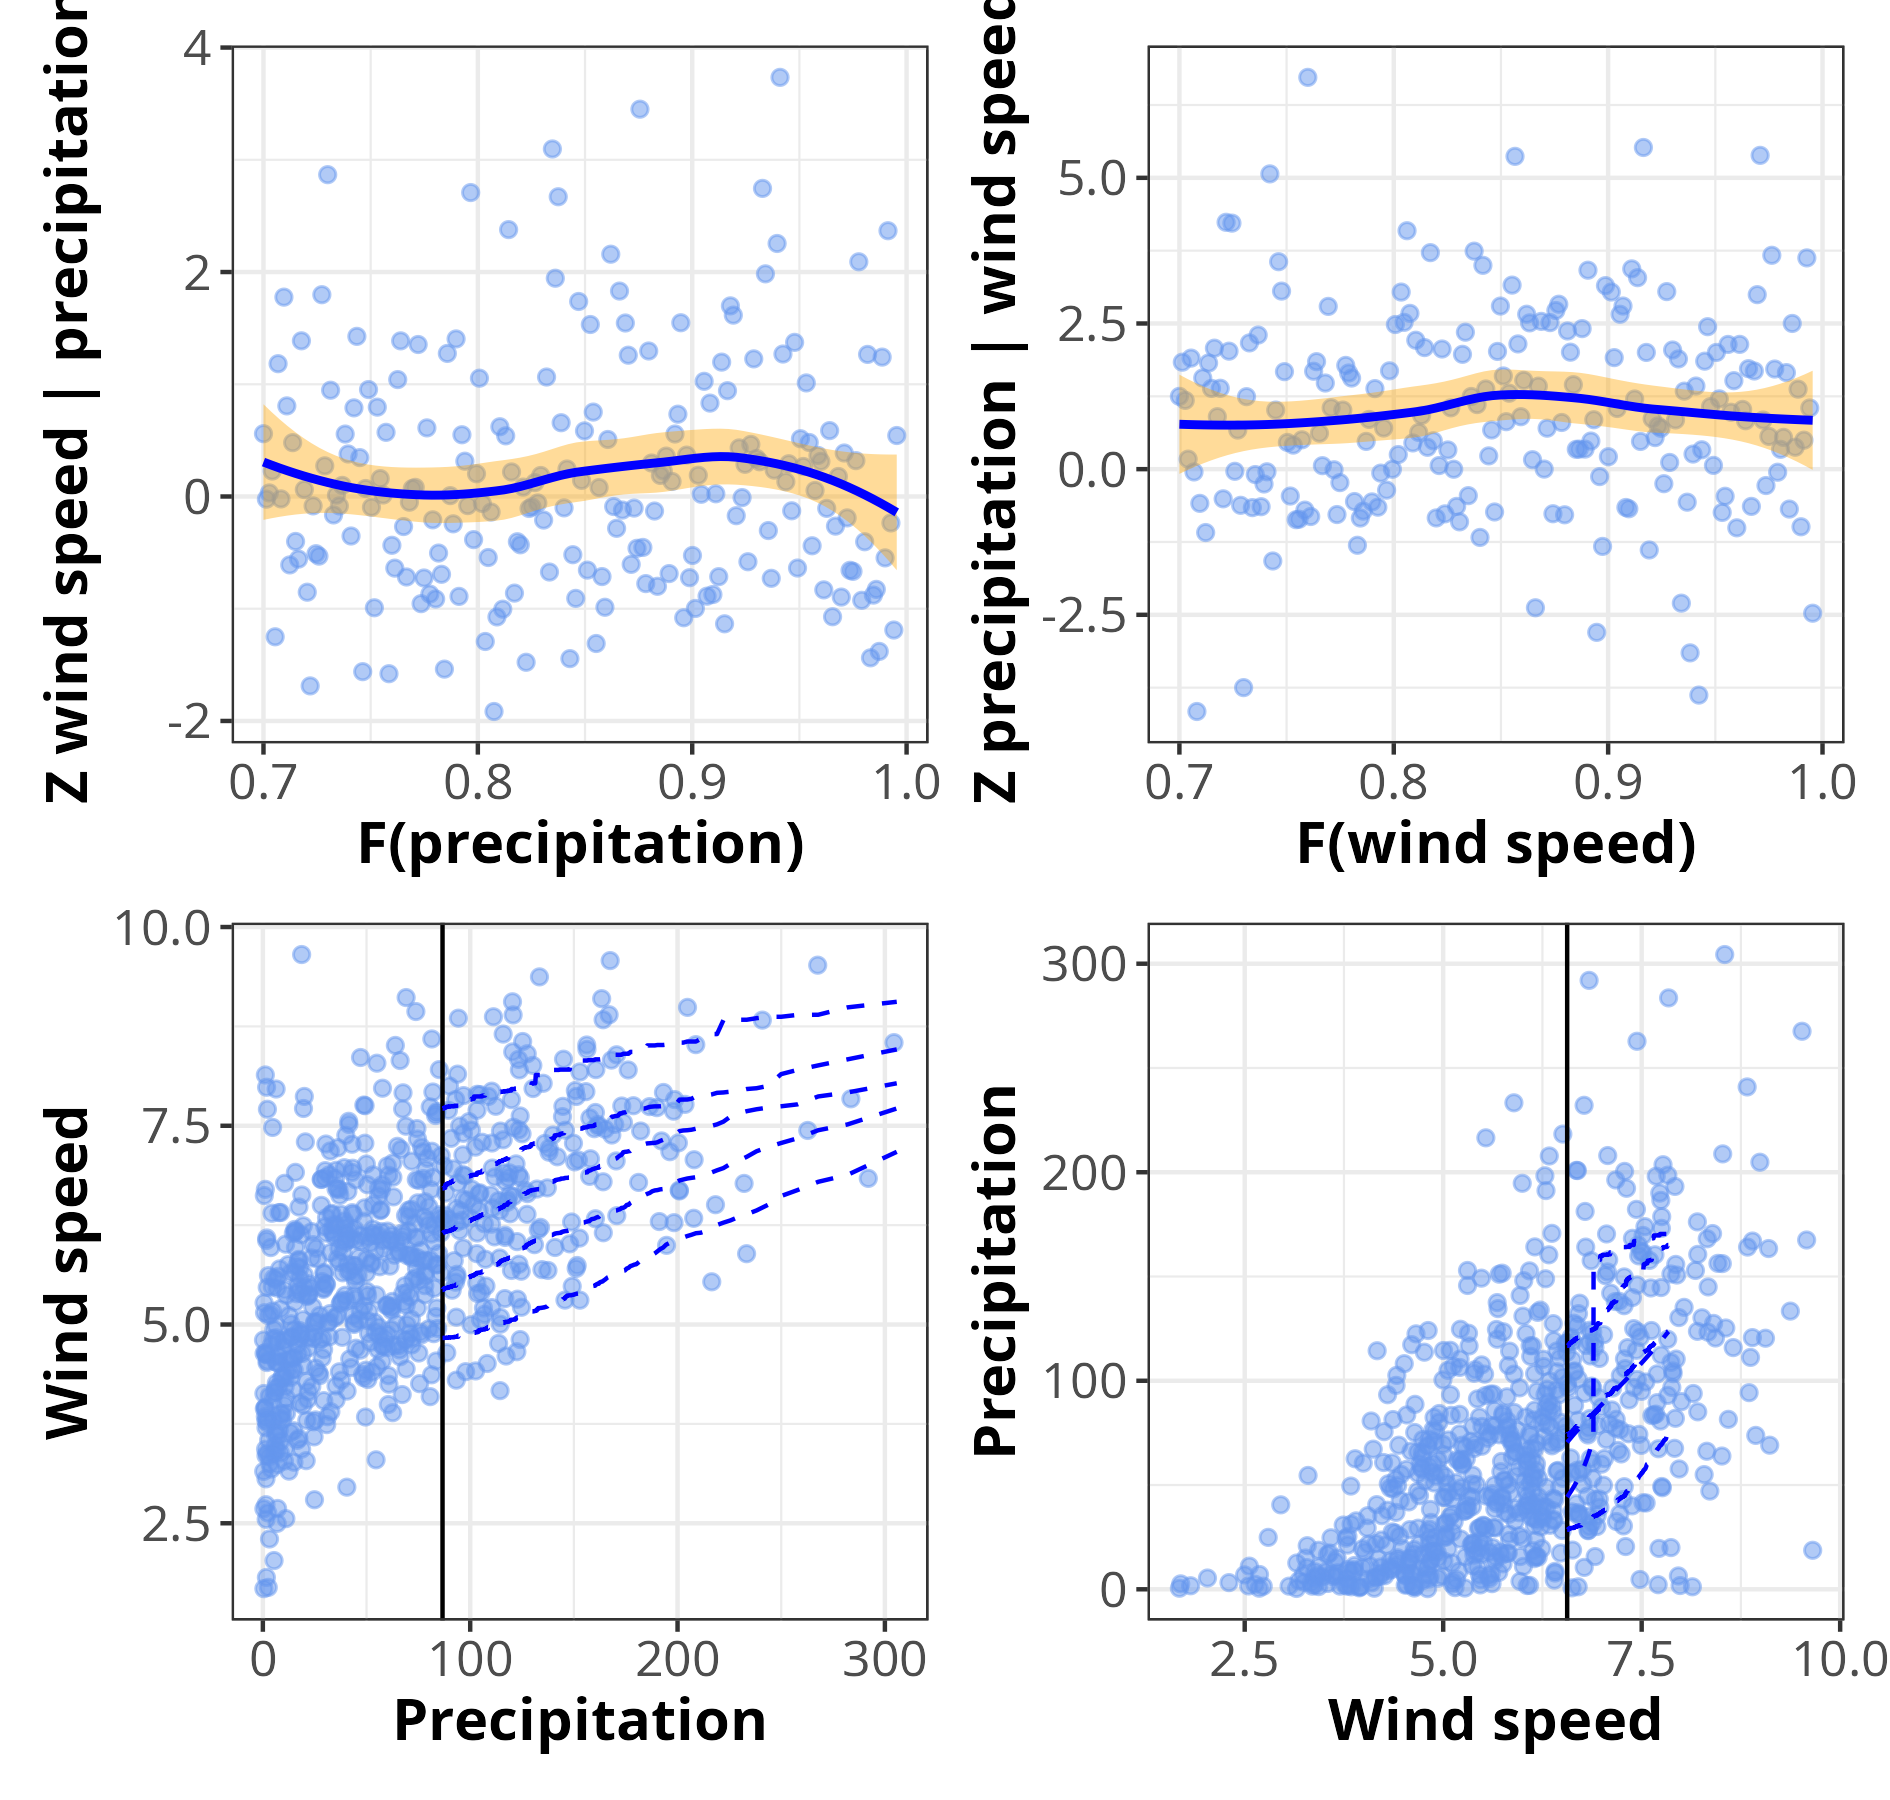
\includegraphics[width = 0.9\linewidth]{plots/048_diag.png}
    \caption{\emph{Test}}
    \label{fig:04_diag}
\end{figure}


\newpage
\section{Clustering for extremes}\label{sec:clustering}

% Mainly lit review on clustering. 
% \begin{itemize}
%   \item Clustering generally done for two reasons: improved explainability and improved parameter estimation. 
%   \item Wealth of literature on clustering for extremes for both of these types. 
% \end{itemize}

\todo{Talk about clustering more? Unsupervised lerning}
Section \ref{subsec:ce_example} has shown how the conditional extremes model is susceptible to uncertainty in its parameter estimates. 
One possible approach to mitigating this susceptibility is through the use of clustering. 
Clustering is generally done for two main reasons.
One purpose is as part of an exploratory analysis, which seek to aid in the interpretation of data. 
The second purpose is to improve parameter estimation in a multidimensional setting, through applying an implicit grouping structure on the data to optimally group together parameter estimates for similar locations or individuals. 
These methods try to use clustering to find a balance in the bias-variance tradeoff inherent in such non-stationary modelling. 
Both purposes have seen widespread usage within extremes, and in this section of the report we perform a literature review on the current landscape of extremal clustering methodologies, which broadly fit within these two categories, so as to consider them in the context of clustering over the conditional extremes model, a currently unexplored problem.

\subsection{Exploratory clustering}

Exploratory clustering, for extremes and elsewhere, mostly focuses on deriving some similarity matrix for a given distance metric, and then using performing some generic clustering algorithm such as k-means or k-mediods on this matrix.

The k-means algorithm \cite{Macqueen1967} defines a cluster centre by some summary statistic, such as the cluster mean.
To give a short description of this simple algorithm, we first randomly select a given number of cluster centres.
Data points are allocated to the cluster whose centre is ``closest'' to that point in terms of some distance metric, the most popular being the squared euclidean distance.
We then re-compute cluster centres by taking some summary statistic such as the mean for the data points allocated to that cluster.
The algorithm then iterates between these cluster allocation and cluster centre computation steps until some stopping criteria is met, such as the cluster membership being stable, or some prescribed number of iterations of the algorithm occurring.

The k-mediods algorithm \cite{Kaufman1987}, in contrast to k-means, defines a cluster centre not by some summary statistics such as the cluster mean, but rather as a data point itself.
This method is particularly useful where it is not suitable to use a non-data point to define a cluster by. 
For example, the mean of a normally distributed variable is itself normal, but no such guarantee is available for, say, a variable with a GPD \cite{Vignotto2021}.
In these situations, using a real data point is often preferred.

There are many examples in the literature of the use of the k-means and k-mediods algorithms for clustering extremes.
Here, we will summarise some examples.

% \begin{itemize}
%   \item First kind mainly focuses on deriving distance matrices for some metric (such as marginal GPD parameters, F-madogram, etc) and applying some classical clustering algorithm such as k-mediods. Can talk about different papers which have done this (multiple references to make here).
%   \item In particular \cite{Vignotto2021} paper matches our application here, would be a promising method to try on the conditional extremes model. In particular, is really simple to implement, but perhaps won't help so much with parameter estimation problem. 
% \end{itemize}

In \citet{Bernard2013}, a clustering algorithm is derived for weekly precipitation maxima for sites across France.
It uses as its distance metric the F-madogram, an extreme-value type of variogram, which are used to estimate spatial correlation. 
The F-madogram forms a copula, and so is completely decoupled from marginal estimates, meaning there is no need to re-estimate a GEV distribution at each site, and it is not required to assume these maxima come from a GEV.
The partitioning-around-mediods (PAM) algorithm, a type of k-mediods algorithm, is used to cluster locations based on the F-madogram. 
Taking mediods ensures that the cluster centre is an actual observation, which allows the maxima to remain maxima and does not apply any averaging or smoothing. 
The PAM algorithm is compared to k-means.
Interestingly, while the algorithm is not given any geographical information, it still produces spatially coherent clusters, in contrast to k-means.
The choice of K, the number of clusters and assessment of clustering quality was made through analysis of the silhouette coefficient, which compares cluster tightness, seeking a small distance within each cluster with cluster dissociation/separation, whereby clusters should be adequately distinct.

\citet{Vignotto2021} proposes a k-mediods algorithm for clustering locations in Great Britian and Ireland characterised by weekly sums of precipitation and weekly maxima of wind speeds.
These variables are transformed to Pareto margins at each location, and a risk function, namely the maximum for both trasformed margins, is used to define extreme observations and partition the bivariate space into three disjoint sets, corresponding to extremal observations for precipitation, wind speed and both. 
The number of points in each of these disjoint sets can be used to compute an empirical estimate for the Kullback-Leibler divergence, a distance used assess the level of similarity between two probability distributions \cite{Kullback1951}, between any two locations.
In this way, a mapping from bivariate to univariate space is made, and a dissimilarity matrix is derived on which the k-medoids algorithm can be applied to perform clustering. 

In \citet{deCarvalho2023}, a ``heteroskedastic clustering'' algorithm is derived, which uses k-means to cluster over a bivariate cluster centre formed from estimators for the extremal index and heteroskedastic function, respectively. 
These metrics can be interpreted as the magnitude and frequency of extreme events, respectively.
They are jointly thresholding to define extreme observations.
This method is particularly useful for clustering extremal time series, since heteroskedastic extremes violate the assumption of IID observations, and may exhibit serial dependence or be drawn from different distributions. 
Accounting for this heteroskedasticity provides an improved clustering solution to competing approaches in the context of time series. 
This method is then applied to stock prices on the London Stock Exchange. 

% \todo{Clustering on polar coordinates!}
All of the methods discussed cluster locations or individuals. 
However, clustering extreme observations is also possible. 
One approach to this problem is through the use of spherical clustering, for which algorithms have been developed in the context of extremes.
Observations are transformed to polar coordinates, decoupling the magnitude and ``direction'' of events into a radial and angular component, respectively.
We can threshold the observations based on their ``radius'' or magnitude, and then cluster observations where extreme events appear to have occurred in tandem or ``concomitantly''.
Again, standard clustering algorithms such as k-means or k-mediods can be used here.
As the data has been projected onto the unit sphere, the cosine similarity metric is a sensible distance measure to cluster with \citep{Fomichov2022, Janen2020, deCarvalho2024}.
Another type of clustering which can be performed in this context is spectral clustering, which takes the eigenvector decomposition of your observations, rather than the observations themselves, projecting them onto a lower dimensional space upon which to do clustering on \citep{Ng2001, Vonluxburg2007}.
Spectral clustering is often preferable to ordinary k-means when data is non-convex or not linearly separable. 

% \subsection{Clustering for improved parameter estimation}
\subsection{Hierarchical clustering}

% \begin{itemize}
%   \item Second kind uses hierarchical modelling and generally produces latent, ``data-driven'' group structure, methods for estimating likelihood can be split between Frequentist methods which use some flavour of EM algorithm, and Bayesian which uses MCMC, in particular \cite{Bottolo2003} and  \cite{Rohrbeck2021}, which use RJMCMC (other methods (possibly from outside extrems) include use of ``stick-breaking prior'' and latent Dirichlet allocation, reference).
%   \item This kind particularly useful for extremes because of lack of data causing ``naive'' marginal $\xi$ values to have large variance (which in turn feeds into estimates of $\alpha$ and $\beta$ for CE model). 
%   \item Earlier paper in this vein is \cite{Cooley2007}, but this only used domain-knowledge to fit two seperate $\xi$ values for different regions (mountainous and plains).
%   \item Talk about Frequentist EM papers for GEV (\cite{Dupuis2023}) and GPD (\cite{Carreau2017}), use variants of EM algorithm. 
%   \item Talk about \cite{Rohrbeck2021}, how it changes RJMCMC algorithm from \cite{Bottolo2003} and uses GPD rather than PP (review both papers), some reasons why it may be an improvement on Frequentist methods:
%     \begin{enumerate}
%       \item Use of priors desirable where data is naturally lacking for extremal context (but may also be shunned for being opinionated?), mention use of Penalised complexity prior for $\xi$ in INLA implementation of GPD. 
%       \item However, specification of priors is sometimes laborious and controversial, and can be difficult to justify. 
%       \item Inference for the \cite{Carreau2017} is quite conceptually difficult, making use of U-statistics for probability weighted moment estimators and in the GEV paper required a  consistency analysis of the QML methods used
%       \item In contrast, inference for Bayesian problem could be seen as somewhat simpler, can be simply expressed through DAG with hyperpriors to enable partial pooling, can more easily limit e.g.\ $\xi$ to more reasonable values, spatial interpolation is easy (but can be made more complex), number of regions/clusters to use can be estimated with within MCMC scheme rather than e.g. cross-validation as in \cite{Carreau2017}.
%       \item Any improvements in computational speed? Can talk about INLA implementation of CE and how it allows for modelling of many regions, opens up use in geostatistical context,
%       \item Probabilistically defines uncertainty around parameter estimates, which is nice, compared to having to define complicated bootstrapping schemes or other methods to quantify uncertainty in Frequentist setting. 
%       \item Also reference context of conditional extremes model, rather than GPD or GEV explicitely (although GPD must be estimated to then estimate CE parameters), probably more easily formulated in hierarchical Bayesian model (how?)
%     \end{enumerate}
%   \item However, Frequentist method doesn't require specification of priors, which is a controversial subject and can be quite laborious.  
% \end{itemize}

% Exploratory clustering, for extremes and elsewhere, mostly focuses on deriving some similarity matrix for a given distance metric, and then using performing some generic clustering algorithm such as k-means or k-mediods on this matrix.

Clustering for improved parameter estimation is often performed through hierarchical clustering.
In hierarchical clustering for extremes, the parameters of our extremal distribution, such as the GPD, are treated as non-stationary, with data split into groups, over which the same parameter estimates are used. 
A grouping structure is sought which balances the bias-variance tradeoff associated with estimating parameters over more or less locations or individuals.

An early example of hierarchical clustering for extremes can be found in \cite{Bottolo2003}, which defined exceedances over a high threshold as generated by a model characterised by a Poisson process $PP(\mu, \sigma, \xi)$.
A Bayesian hierarchical model is proposed with a separate hierarchical mixture prior for each of the parameters of the PP, each having a specific latent group structuring.
The use of a mixture and parameter-specific prior assumes that parameters are IID according to some finite-mixture distribution, and gives this model great flexibility in its group structure and parameter estimation. 
The model also allows the incorporation of prior knowledge into these priors, which is useful in the context of extremes due to the innate scarcity of extremal data.
The model is estimated using a Reversible Jump MCMC (RJMCMC) algorithm, which allows for the estimation of the number of clusters, rather than requiring it to be pre-determined, as in k-eans clustering. 

Another early example is \citet{Cooley2007}, which modelled return levels for extreme precipitation in Colorado.
Separate hierarchical models were used to estimate for intensity and frequency of extremes for a given location using the GPD and the binomial distribution, respectively.
Both of these fitted distributions incorporate latent spatial process characterised by geographical and climatological covariates using a Gaussian process. 
Hyperparameters which drive the latent spatial process are specified.
Unlike \cite{Bottolo2003}, grouping of locations was not latent, and the Deviance Information Criterion (DIC) was used to compare models with different covariate forms for the shape and scale parameters of the GPD.
Interestingly, the best model used two separate shape parameters for ``mountainous'' and ``planes'' regions, performing better than models which estimated the shape parameter using covariates and for fewer locations, highlighting the instability inherent in this parameter.

% In a more recent, frequentist example, \citet{Carreau2017} derives a model which uses covariates to estimate the scale parameter for a conditional mixture of GPDs with subregions defined by a constant shape parameter.
In a more recent, frequentist example, \citet{Carreau2017} derives a model which utilises a conditional mixture of GPDs with subregions defined by a constant shape parameter.
Building on the findings of \cite{Cooley2007} that the shape parameter is unstable when modelled with covariates, only the scale parameter is estimated as a function of covariates, and clusters are formed over which the shape parameter is held constant. 
Inference is performed through an adapted expectation-maximisation (EM) algorithm. 
The E-step estimates the partition of each location, while the M-step estimates the probability of subregion membership used in the mixture GPD, as well as the model parameters.
The number of subregions to partition the data into was chosen by out-of-sample cross-validation using three different loss functions, including the Anderson-Darling statistic, which is used to compare probability distributions and is particularly sensitive to tail deviation.

In \cite{Dupuis2023}, an EM algorithm is derived for identifying group structure and group-specific model parameters for GEV distributed panel data.
Each parameter of the GEV is modelled as a function of covariates. 
The EM algorithm in question is really made up of two E-steps, which iteratively estimate the group structure and assignment and the individual rregression equations, respectively
The grouping is latent and ``data-driven'', rather than based on domain knowledge. 
Stronger dependence in the data is found to help group identification because it reduces the variance among individuals in the same group, but it gives worse quantile estimates. 
A simulation study using this model was performed, and applications to financial risk, extreme temperature and flood risk data were shown to be effective, and superior to methods using groupings based on domain knowledge.

\todo{bayesian clustering!}

Another, more recent example of Bayesian hierarchical clustering is in \cite{Rohrbeck2021}, specifically applied to hydrological variables. 
This clustering algorithm derives a separable likelihood function defined by a marginal and dependence component.
% The marginal component consists of a GPD, over which constraints are set using priors so that the parameters of the fitted GPDs are more similar for locations within the same cluster than those in different clusters. 
The marginal component consists of a cluster-specific GPD.
The dependence component uses the $\chi$ statistic, and constraints are applied to this statistic so that locations in the same cluster have more similar $\chi$ values than those in other clusters, and also that this similarity is a function of and decreases with distance.
Priors are set so that each cluster is spatially contiguous, and each site is assigned to the closest cluster centre in terms of their geographical distance from each other.
This algorithm uses a similar RJMCMC algorithm to \cite{Bottolo2003} for inference, where the number of clusters it itself estimated rather than supplied, and cluster membership is represented as a random variable. 


\newpage
\section{Discussion} \label{sec:discussion}

In this section, we summarise and conclude the work in this report. 
We also explore several promising avenues for future work within the scope of clustering methods for the conditional extremes model, both in the short and long-term, which we hope to pursue over the next three years of PhD research. 

\section{Summary and conclusions}

% Introduction
In this report, we began in section \ref{sec:intro} with an introduction to the field of EVT and why it is useful.
% We described how EVT is used for modelling both univariate extreme data, and in particular how it can be extended to model the dependence structure of a multivariate dataset, with some examples from the literature. 
We described how EVT is used in modelling univariate extreme data, and also in particular how it important in a multivariate extremes setting to model the dependence structure in our data, for which we have used the conditional extremes model.
We have provided numerous examples from the literature of the use of EVT in both univariate and multivariate contexts. 

% Motivating example
In section \ref{sec:motivating}, we introduced our motivating example of extreme precipitation and wind speed data from 52 weather stations in Ireland. 
This example serves to illustrate the univariate and dependence models described in this report, and also to shed some light on the possible shortcomings in these methods as they currently stand.

% Univariate
We described the POT method for defining extreme data in a univariate setting in \ref{sec:uni}, and how we can use the GPD to model this data. 
Foundational modelling techniques used under this framework were described, including methods for both graphical and automatic threshold selection and model diagnostic tools. 
We showed how the model can be extended to handle non-stationary data, particularly through the use of GAMs, which allow for the inclusion of non-linear spatial effects to reflect the  geographical heterogeneity in extremal patterns in our GPD parameter estimates. 
These methods were put into practice for our motivating example by successfully fitting GPDs to both precipitation and wind speed, producing sensible results for both. 
To summarise the results of this modelling, more extreme precipitation is to be anticipated further West in the country, while more severe wind speeds are to be expected along coastal regions than inland, particularly for the East coast surrounding Dublin. 
\todo{Was this in line with any other modelling, such as Vignotto2021?}
\todo{Maybe some physical reason why we get more extreme further West? W/ reference (see Vignotto)}

% Conditional Extremes
\todo{Reference some max-stable process paper in 4.1!}
\todo{have section before all references to sections}
In section \ref{sec:ce}, we gave a general introduction to dependence modelling for extremes, its usefulness, and some of the types of models used in the literature for this purpose. 
The dependence model which is more flexible than many alternatives that we particularly focus on is the conditional extremes model, which combines a semiparametric model for multiple univariate extremes with a semiparametric regression model for their corresponding dependence structure.
This model and methods for its estimation and use were described in detail. 
Several extensions to adapt the model to work with covariates and in possibly high-dimensional spatial and spatio-temporal settings were also mentioned. 
Finally, the conditional extremes model was applied to our motivating example, with some mixed results. 
Exploratory analysis through the $\chi$ and $\bar{\chi}$ statistics implied that there may be some extremal dependence between precipitation and wind speed in Ireland, becoming more pronounced further West.
Bootstrapping and profile likelihoods revealed that the parameter estimates for the conditional extremes model were susceptible to high uncertainty at many locations, which made interpretation difficult. 
A makeshift solution to this problem was to fix the $\beta$ parameter to a single value, $0.1$, and have the model only estimate the $\alpha$ parameter, which as the slope parameter of the regression line corresponds to the strength of dependence between precipitation and extreme wind speeds, and vice versa.
This adaption did reveal some patterns in the data.
In particular, our results agreed with the exploratory analysis in that extremal dependence between precipitation and wind speed did appear to increase further West in Ireland. 
Also, at stations where high extremal dependence for precipitation on wind speed was observed, often the wind speed also had high extremal association with precipitation. 
However, this solution was quite makeshift, and does not make up for some of the outstanding issues with parameter uncertainty which the model experiences in this application. 
As we did not use a non-stationary conditional extremes model here, one possible extension to this analysis would be to incorporate spatial covariates for our regression parameters. 
Another approach, which we focused on in greater detail, is the use of clustering.

% Clustering
We performed a literature review, looking at the numerous existing applications of clustering for extremes.
In particular, extremal clustering falls into two categories.
The first kind typically derives some dissimilarity matrix via some distance metric, such as euclidean distance or KL divergence, over either the parameters of an extreme value distribution or some derived summary, and uses either the k-means or k-mediods algorithms to perform clustering. 
This type of clustering is more typically used as part of an exploratory analysis. 
The second type of clustering focuses on deriving hierarchical models with latent group structures which improve parameter estimation when using either the GPD or GEV, possibly in combination with some measure of dependence.
In frequentist settings, these models often use some form of EM algorithm, while in a Bayesian setting the use of a RJMCMC algorithm is one possible approach.
Both approaches have their respective merits, with the need for specifying priors for Bayesian analysis seen as both a strength, especially in the context of extremes where data is naturally rare, and a possible weakness, in that prior specification is often a difficult and hazardous task, even when uninformative priors are sought. 
From this literature review of extremal clustering, some interesting avenues for future research in clustering for the conditional extremes model arise. 

% Notes:
% Bayesian CE: how do we write the likelihood?
% What priors will need to be used? Priors on tanh^-1(alpha), log(beta) (?)
% Gaussian assumption for residuals, see how well this holds up
% Mixture of Gaussians may work well, but would assume a linear trend (???) 
% ALso want to work on computation

\subsection{Future work}

% Future work:
% \begin{itemize}
  % \item Try general clustering (k-means, k-medoids) on conditional extremes models
  % \item Another more sophisticated but also quite simple area of future work would be to try to implement \citet{Vignotto2021} paper method on Ireland dataset for conditional extremes model, as context of bivariate wind speed and precipitation dependencies at different locations is quite similar to the context of the paper.
  % \item This model has some limitations in that it may not be extended past bivariate case, doesn't use spatial information, must manually refit CE model with clustering, questionable basis on which to perform clustering for improved parameter estimation  \todo{See discussion in Vignotto paper to see what they had to say about this}.
  % \item Potential to try Bayesian clustering approach similar to \citet{Rohrbeck2021}, will involve deriving likelihood for CE model and priors for parameter values. 
  % \item Later, can extend clustering to spatial and spatio-temporal CE from \citep{Tawn2018, Simpson2021}.
% \end{itemize}

Firstly, we would like to apply some general clustering through the use of the k-mediods or k-means algorithm on the parameters of the conditional extremes model. 
However, some challenges are likely to stand in the way. 
Particularly, the choice of distance metric poses a difficulty. 
This prospective distance metric must be sensible and valid in the context of the parameters of the conditional extremes model, for which something as simple as euclidean distance will not be sufficient.

It would also be interesting to try applying the method of \cite{Vignotto2021} to our the conditional extremes model in our motivating example. 
The methodology behind this approach is rather simple, and the application is quite similar to our own, also looking at bivariate extremal dependence between precipitation and wind speed for Ireland, as well as the United Kingdom.
In this paper, they compute the KL divergence for some partitioned bivariate space of precipitation and wind speed readings at different locations, projecting into univariate space over which locations can be compared. 
We could take a similar approach, although it must be noted that we have two parameters for the conditional extremes model for both precipitation and wind speed, so it may be that we focus on just clustering on $\alpha$ at first, fixing $\beta$ as we did in the analysis in this report. 
We could also simply simply compare the results of this method with that of our own prospective clustering algorithm.

A more long term goal would be to explore the use of the Bayesian hierarchical approach using an RJMCMC algorithm, first used in the extremes in \citet{Bottolo2003} for mixture models, and then used more closely to our interests for dependence modelling in \citet{Rohrbeck2021}, using the $\chi$ statistic.
There are several considerations to be made when exploring such an approach. 
As in any Bayesian model, a likelihood will need to derived, and suitable priors for $\alpha$ and $\beta$, or $\tanh^{-1}{\alpha}$ and $\tanh^{-1}(\beta)$ or $logit(\beta)$, as in \citet{Winter2016} and \cite{Richards2023} will need to be specified. 
In the conditional extremes model, the standardised residuals $\bm{Z}$ are assumed to come from a multivariate normal distribution. 
After implementing and testing our prospective Bayesian clustering approach, we may consider whether the assumption of Z being normally distributed may be relaxed.

Should these approaches produce some promising results for the stationary conditional extremes model, we may also attempt to extend our clustering algorithm(s) to the non-stationary, spatial and spatio-temporal conditional extremes models.
These extensions may require the improvement of the computational implementation of existing algorithms to prove realistic.

\section*{Code Availability}

\todo{Make sure this is public while TFR report is being reviewed!}
The code for this analysis is available at \url{https://github.com/potoole7/TFR}.
A ``fork'' of the \texttt{texmex} package, available at \url{https://github.com/potoole7/texmex}, was required to add certain functionality, such as fixing $\beta$ values and only estimate $\alpha$, and to use the marginal model from \texttt{evgam} rather than the stationary marginal models used in \texttt{texmex}.

\todo{Number references!}
\todo{Add links for references, if not already present}
\todo{Triple check!! Why are some titles in italics?}

\newpage
\bibliography{library}

\end{document}
